% do not change these two lines (this is a hard requirement
% there is one exception: you might replace oneside by twoside in case you deliver 
% the printed version in the accordant format
\documentclass[11pt,titlepage,oneside,openany]{book}
\usepackage{times}
\usepackage{caption}
\usepackage{longtable}
\usepackage{float}
\usepackage{pgfplots}
\pgfplotsset{width=11.5cm,compat=1.9}
\usepackage{xcolor, colortbl}
\usepackage{graphicx}
\usepackage{svg}
\usepackage{latexsym}
\usepackage{amsmath}
\usepackage{amssymb}
\usepackage{glossaries}
\usepackage{lscape}
\usepackage{interval}
\usepackage{longtable}
\usepackage{ntheorem}
\usepackage{comment}
\usepackage{caption}
\usepackage{tabularx}
\usepackage[colorlinks,pdfpagelabels,pdfstartview = FitH,bookmarksopen = true,bookmarksnumbered = true,linkcolor = black,plainpages = false,hypertexnames = false,citecolor = black]{hyperref}
%\usepackage[table,xcdraw]{xcolor}
% \usepackage{paralist}
\usepackage{tabularx}
\usepackage{amssymb}
\usepackage{algorithmic}

% this packages are useful for nice algorithms
\usepackage{algorithm}
\usepackage{algorithmic}

\hypersetup{colorlinks=true,urlcolor=blue}
% well, when your work is concerned with definitions, proposition and so on, we suggest this
% feel free to add Corrolary, Theorem or whatever you need


\newtheorem{definition}{Definition}
\newtheorem{proposition}{Proposition}

\DeclareMathOperator*{\argmax}{arg\,max}
% its always useful to have some shortcuts (some are specific for algorithms
% if you do not like your formatting you can change it here (instead of scanning through the whole text)
\renewcommand{\algorithmiccomment}[1]{\ensuremath{\rhd} \textit{#1}}
\def\MYCALL#1#2{{\small\textsc{#1}}(\textup{#2})}
\def\MYSET#1{\scshape{#1}}
\def\MYAND{\textbf{ and }}
\def\MYOR{\textbf{ or }}
\def\MYNOT{\textbf{ not }}
\def\MYTHROW{\textbf{ throw }}
\def\MYBREAK{\textbf{break }}
\def\MYEXCEPT#1{\scshape{#1}}
\def\MYTO{\textbf{ to }}
\def\MYNIL{\textsc{Nil}}
\def\MYUNKNOWN{ unknown }
% simple stuff (not all of this is used in this examples thesis
\def\INT{{\mathcal I}} % interpretation
\def\ONT{{\mathcal O}} % ontology
\def\SEM{{\mathcal S}} % alignment semantic
\def\ALI{{\mathcal A}} % alignment
\def\USE{{\mathcal U}} % set of unsatisfiable entities
\def\CON{{\mathcal C}} % conflict set
\def\DIA{\Delta} % diagnosis
% mups and mips
\def\MUP{{\mathcal M}} % ontology
\def\MIP{{\mathcal M}} % ontology
% distributed and local entities
\newcommand{\cc}[2]{\mathit{#1}\hspace{-1pt} \# \hspace{-1pt} \mathit{#2}}
\newcommand{\cx}[1]{\mathit{#1}}
% complex stuff
\def\MER#1#2#3#4{#1 \cup_{#3}^{#2} #4} % merged ontology
\def\MUPALL#1#2#3#4#5{\textit{MUPS}_{#1}\left(#2, #3, #4, #5\right)} % the set of all mups for some concept
\def\MIPALL#1#2{\textit{MIPS}_{#1}\left(#2\right)} % the set of all mips

\makeglossaries

\newglossaryentry{t_d}{%
    name={t_d},%
    description={Elapsed game time in days}%
}

\newglossaryentry{t_y}{%
    name={t_y},%
    description={Elapsed game time in years}%
}

\newglossaryentry{cs}{%
name={cs},%
description={Customer Satisfaction}%
}

% HR Glossary
\newglossaryentry{QoW}{%
name={QoW},%
description={Quality of Work}%
}

\newglossaryentry{EB}{%
name={EB},%
description={Employer Branding}%
}

%Glossary Finance
\newglossaryentry{EBIT}{%
name={EBIT},%
description={earnings before interest and tax}%
}
\newglossaryentry{NOPAT}{%
name={NOPAT},%
description={net operating profit after tax}%
}
\newglossaryentry{tSR}{%
name={tSR},%
description={totalSalesRevenue}%
}
\newglossaryentry{E}{%
name={E},%
description={Set of hired Employees}%
}

\newglossaryentry{EN}{%
name={EN},%
description={Set of hired engineers}%
}

\newglossaryentry{TR}{%
name={TR},%
description={set of trainings in the last period}%
}
\newglossaryentry{tHRC}{%
name={tHRC},%
description={totalHRCosts}%
}
\newglossaryentry{tMC}{%
name={tMC},%
description={totalMarketingCosts}%
}
\newglossaryentry{cc}{%
name={cc},%
description={CapCoins}%
}
\newglossaryentry{S}{%
name={S},%
description={requested loanAmount}%
}
\newglossaryentry{t}{%
name={t},%
description={term for loan (duration)}%
}
\newglossaryentry{a}{%
name={a},%
description={annual repayment for loan}%
}
\newglossaryentry{i}{%
name={i},%
description={interest rate for loan (interestsLoan)}%
}

%Glossary ecoIndex
\newglossaryentry{eI}{%
name={eI},%
description={ecoIndex}%
}

% Glossary Production
\newglossaryentry{P}{%
name={P},%
description={Set of products}%
}
\newglossaryentry{C_pC}{%
    name={C_pC},%
    description={Set of components categories for a product category}%
}
\newglossaryentry{pC}{%
    name={pC},%
    description={product category}%
}
\newglossaryentry{mE}{%
name={mE},%
description={manufactureEfficiency}%
}
\newglossaryentry{tPQ}{%
name={tPQ},%
description={totalProductQuality}%
}
\newglossaryentry{pPP}{%
name={pPP},%
description={productionProcessProductivity}%
}
\newglossaryentry{pT}{%
name={pT},%
description={productionTechnology}%
}
\newglossaryentry{tEQoW}{%
name={tEQoW},%
description={totalEngineerQualityofWork}%
}
\newglossaryentry{tEP}{%
name={tEP},%
description={totalEngineerProductivity}%
}
\newglossaryentry{pA}{%
name={pA},%
description={processAutomation}%
}
\newglossaryentry{sS}{%
name={sS},%
description={systemSecurity}%
}
\newglossaryentry{tCC}{%
name={tCC},%
description={totalComponentCost}%
}
\newglossaryentry{tPC}{%
name={tPC},%
description={totalProductCost}%
}
\newglossaryentry{sFig}{%
name={sFig},%
description={salesFigures}%
}
\newglossaryentry{mC}{%
name={mC},%
description={machineCapacity}%
}
\newglossaryentry{pTF}{%
name={pTF},%
description={productionTechnologyFactor}%
}
\newglossaryentry{pAF}{%
name={pAF},%
description={processAutomationFactor}%
}
\newglossaryentry{nPP}{%
name={nPP},%
description={numberProducedProducts}%
}
\newglossaryentry{RDF}{%
name={RDF},%
description={Research and Development Factor}%
}

%Glossary Marketing
\newglossaryentry{eB}{%
name={eB},%
description={employerBranding}%
}
\newglossaryentry{cI}{%
name={cI},%
description={companyImage}%
}
\newglossaryentry{tJS}{%
name={tJS},%
description={totalJobSatisfaction}%
}
\newglossaryentry{CSR}{%
name={CSR},%
description={Corporate Social Responsibility}%
}
\newglossaryentry{oS}{%
name={oS},%
description={Original Scale}%
}
\newglossaryentry{PInt}{%
name={PInt},%
description={Personal Interview}%
}
\newglossaryentry{TInt}{%
name={TInt},%
description={Telephone Interview}%
}
\newglossaryentry{MSur}{%
name={MSur},%
description={Mail survey}%
}
\newglossaryentry{OSur}{%
name={OSur},%
description={Online survey}%
}

%Glossary Logistic
\newglossaryentry{eIT}{%
name={eIT},%
description={ecoIndexTruck}%
}
\newglossaryentry{qIT}{%
name={qIT},%
description={qaulityIndexTruck}%
}
\newglossaryentry{pPT}{%
name={pPT},%
description={purchasePriceTruck}%
}
\newglossaryentry{nT}{%
name={nT},%
description={numberTrucks}%
}
\newglossaryentry{T}{%
name={T},%
description={Set of purchased trucks}%
}
\newglossaryentry{cF}{%
name={cF},%
description={capacityInternalLogisticFleet}%
}
\newglossaryentry{iLI}{%
name={iLI},%
description={internalLogisicIndex}%
}
\newglossaryentry{fTC}{%
name={fTC},%
description={fixTruckCost}%
}
\newglossaryentry{tTC}{%
name={tTC},%
description={totalTruckCost}%
}
\newglossaryentry{fCD}{%
name={fCD},%
description={fixCostsDelivery}%
}
\newglossaryentry{vCD}{%
name={vCD},%
description={variableCostsDelivered }%
}
\newglossaryentry{cED}{%
name={cED},%
description={costExternalDelivery }%
}
\newglossaryentry{tDC}{%
name={tDC},%
description={totalDeliveryCost}%
}
\newglossaryentry{dP}{%
name={dP},%
description={deliveredProducts}%
}
\newglossaryentry{eIP}{%
name={eIP},%
description={ecoIndexPartner}%
}
\newglossaryentry{qIP}{%
name={qIP},%
description={qualityIndexLogisticPartner}%
}
\newglossaryentry{cCLP}{%
name={cCLP},%
description={contractualCostLogisticPartner}%
}
\newglossaryentry{tLC}{%
name={tLC},%
description={totalLogisticCost}%
}
\newglossaryentry{cL}{%
name={cL},%
description={costLogistic}%
}
\newglossaryentry{vCDE}{%
name={vCDE},%
description={variableCostDeliveryExternal}%
}
\newglossaryentry{rIP}{%
name={rIP},%
description={reliabilityLogisticPartner}%
}
\newglossaryentry{sF}{%
name={sF},%
description={shippingFee}%
}
\newglossaryentry{eF}{%
name={eF},%
description={ecoIndexFleet}%
}
\newglossaryentry{qF}{%
name={qF},%
description={qualityIndexFleet}%
}
\newglossaryentry{eLI}{%
name={eLI},%
description={externalLogisticIndex}%
}
\newglossaryentry{lI}{%
name={lI},%
description={logisticIndex}%
}

%Glossary Support
\newglossaryentry{cST}{%
name={cST},%
description={costSupportType}%
}
\newglossaryentry{tSTQ}{%
name={tSTQ},%
description={totalSupportTypeQuality}%
}
\newglossaryentry{tSQ}{%
name={tSQ},%
description={totalSupportQuality}%
}
\newglossaryentry{qSP}{%
name={qSP},%
description={qualitySupportPartner}%
}
\newglossaryentry{tSC}{%
name={tSC},%
description={totalSupportCost}%
}
\newglossaryentry{cSP}{%
name={cSP},%
description={costSupportPartner}%
}
\newglossaryentry{sTQ}{%
name={sTQ},%
description={supportTypeQuality}%
}
\newglossaryentry{ST}{%
name={ST},%
description={Set of offered support types}%
}

%Glossary Warehouse
\newglossaryentry{bCW}{%
name={bCW},%
description={buildingCostWarehouse}%
}
\newglossaryentry{rCW}{%
name={rCW},%
description={rentalCostWarehouse}%
}
\newglossaryentry{cW}{%
name={cW},%
description={capacityWarehouse}%
}
\newglossaryentry{vSC}{%
name={vSC},%
description={variableStorageCost}%
}
\newglossaryentry{fCW}{%
name={fCW},%
description={fixCostWarehouse}%
}
\newglossaryentry{tCWH}{%
name={tCWH},%
description={totalCapacityWarehouse}%
}
\newglossaryentry{cWH}{%
name={cWH},%
description={costsWarehouses}%
}
\newglossaryentry{nWH}{%
name={nWH},%
description={numberWarehouses}%
}
\newglossaryentry{nRWH}{%
name={nRWH},%
description={numberRentedWarehouses}%
}
\newglossaryentry{sU}{%
name={sU},%
description={storedUnits}%
}
\newglossaryentry{sC}{%
name={sC},%
description={storageCosts}%
}
\newglossaryentry{fSWH}{%
name={fSWH},%
description={freeStorage}%
}
\newglossaryentry{tWC}{%
name={tWC},%
description={totalWarehouseCost}%
}

%Glossary Demand 
\newglossaryentry{sCP}{%
name={sCP},%
description={sumComponentPrices}%
}
\newglossaryentry{dPR}{%
name={dPR},%
description={demandPrice}%
}
\newglossaryentry{sP}{%
name={sP},%
description={salesPrice}%
}
\newglossaryentry{dA}{%
name={dA},%
description={demandAmount}%
}
\newglossaryentry{mS}{%
name={mS},%
description={marketShare}%
}
\newglossaryentry{tMS}{%
name={tMS},%
description={totalMarketShare}%
}
\newglossaryentry{sFP}{%
name={sFP},%
description={salesFigureProduct}%
}
\newglossaryentry{dPC}{%
name={dPC},%
description={demandPercentage}%
}
\newglossaryentry{gP}{%
name={gP},%
description={gamePopulation}%
}
\newglossaryentry{tSQOW}{%
name={tSQOW},%
description={totalSalesQualityOfWork}%
}


%Glossary Procurement 
\newglossaryentry{tBCP}{%
name={tBCP},%
description={timeBasedComponentPrice}%
}
\newglossaryentry{iCP}{%
name={iCP},%
description={initialComponentPrice}%
}
\newglossaryentry{tProcureQ}{%
name={tProcureQ},%
description={totalProcurementQuality}%
}
\newglossaryentry{C_p}{%
name={C_p},%
description={Set of components of a product P}%
}
\newglossaryentry{c}{%
name={c},%
description={component}%
}

%Glossary CustomerSatisfaction 
\newglossaryentry{cS}{%
name={cS},%
description={customerSatisfaction}%
}
\newglossaryentry{dSL}{%
name={dSL},%
description={daysSinceLaunch}%
}
\newglossaryentry{pDA}{%
name={pDA},%
description={periodicDemandAmount}%
}
\newglossaryentry{oA}{%
name={oA},%
description={overallAppeal}%
}
\newglossaryentry{aOA}{%
name={aOA},%
description={averageOverallAppeal}%
}
\newglossaryentry{JSS}{%
name={JSS},%
description={Job Satisfaction Score}%
}


\begin{document}

\pagenumbering{roman}
% lets go for the title page, something like this should be okay
\begin{titlepage}
	\vspace*{2cm}
  \begin{center}
   {\Large Capitalism X\\}
   \vspace{2cm} 
   {Handbook \& Documentation\\}
   \vspace{2cm}
   {presented by\\
   Philipp Epstein, 1624235 \\
    Daniel G\"otz, 1533213 \\
Maike Jansen, 1624246\\
Nike Klaubert, 1624393\\
Salih \"Ozdemir, 1373080 \\
Livja Papuciu, 1625283\\
Janine Salomon, 1624268\\
Steffen Waldmann, 1418219\\
   }
   \vspace{1cm} 
   {submitted to the\\
    Data and Web Science Group\\
    Prof.\ Dr.\ Heiner Stuckenschmidt\\
    University of Mannheim\\} \vspace{2cm}
   {March 2019}
  \end{center}
\end{titlepage} 

% no lets make some add some table of contents
\tableofcontents
\newpage
\printglossary[style=long]
\listoffigures

\listoftables

% evntuelly you might add something like this
% \listtheorems{definition}
% \listtheorems{proposition}

\newpage
% okay, start new numbering ... here is where it really starts
\pagenumbering{arabic}

\chapter{From a Small Start-Up to a Global Enterprise}
\label{cha:intro}
\section{What to expect from Capitalism X}
\label{expectation}
%Nike
Have you ever wanted to test out your economic skills and entrepreneurial spirit? Did you ever wish to take action and do things your way? Did you ever think that with the steering wheel in your hand, you'd give a company a whole new direction and possibility to rise? 

Capitalism X now gives you the possibility to become CEO! This business simulation game, which is equally fun and educative, gives you the chance to prove your successful way of managing a company through decades. You are going to start with a small technology company and, with your sophisticated input, you can build up an enterprise.

The goal of this interactive business simulation game is simple: Maximize your company's net worth! As a CEO you will have to take care of multiple issues, that occur in daily business, such as defining your product portfolio, controlling your financial status, managing employees and so on. However, unforeseen events might suddenly occur! In these cases, you can prove your decision-making abilities and guide your company through delicate situations. 

With Capitalism X you can expect a game which let you experience the core processes of a corporation. Activities in this game match the processes which are derived from real world companies. You will start as a start-up and develop the company through smart decisions and actions to a big corporation. Although the decisions you will make are based on simplified assumptions, the overall complexity is based on a real world scenario and will give you an overview about the inter-dependencies in a company.
 
\section{Player's Role}
%Maike
You will take on the role of CEO for either a start-up or a mid-sized company which is about to fail. During your career, you will encounter several obstacles and lead the business. So, you will slip into various roles, such as head of human resources, production or logistics, in order to take the necessary measures to run a successful business. Daily tasks include hiring, firing, motivating and training employees, innovating and manufacturing products, deciding on the product portfolio, dealing with government issues and taking financial figures into account. 

In summary, you will decide on all the features provided in this game. Your decisions are then integrated into finance, human resources, procurement, production, warehousing, logistics and marketing and will finally affect the performance of your company.

\section{Setting and Storyline}
\label{SettingStory}

Capitalism X is created relying on a progressive game-play modality, meaning that the game will start as a one-man business with you as the only employee, and then evolve step by step, by employing, producing, expanding, buying and selling until the end goal is achieved, which is to transform the initial company into a large corporation. 

\subsubsection{Setting}
The setting of our game is in a fictional country, which we have designed after having drawn some simple parallels with real countries or cities. These parallels mean that our country has the most important features, that allow an economy to grow. Hence, we divided our map elements into functional and non-functional elements. Where functional buildings are the ones you can interact with, for instance, taking a loan in a bank, advertising in a media building, hiring employees in a job center, etc.  To give another illustration, our fictional country operates with the outside world through the simulation of a harbor in the early stages of the game and then it will be possible to unlock an airport. Whereas non-functional buildings are objects with a decorative purpose to make the map look and feel  more realistic to the user’s perception. The complete list of functional and non-functional buildings can be found in table \ref{table:map-el}. 
\begin{table}[ht]
\centering
\begin{tabular}{r|l}
\hline 
 Functional Elements & Non-functional Elements\\
\hline \hline
 Bank & City Center  \\
 Government Building & Infrastructure \\
 Job Center & Sea/River \\
 Harbour & Park/Art Center  \\
 Competitor Buildings & \\
\hline
\end{tabular}
\caption{Functional/Non-functional map elements}
\label{table:map-el}
\end{table}


Regarding the time-frame, our game simulation is going to be set between $1990$ and $2017$. We have collected data for several factors that influence the economy and each year in the real world is represented by $365$ seconds. This means that the total number of hours you can play Capitalism X is approximately $2.7$ hours. 
On the other hand, we have to emphasize the parameters can change daily, monthly, quarterly or yearly  asynchronously to user inputs.

During the entire time-span of the game, there will be a democratic government that operates and interacts with the game environment. The government can also intervene to impose laws, taxes and additional measures, if the company is not compliant to the current regulations. 

Furthermore an additional unique element in this game simulation is the currency. Capitalism X has its own currency, which is the CapCoin (\gls{cc}), and every function within the game is adapted to operate with this currency.

\subsubsection{Storyline}
 The storyline that you will be operating in would be that of managing a technology company, which you have founded as a start-up. You will be able to choose which employees to hire, which products to manufacture,  how to set the price on these products, etc. These options and many more comprise scenarios and decisions you will have to face in order to have a successful company. Having said this, it is evident that your role will be that of the CEO of the company. By assuming this role you will be able to control all the major departments of the company such as, HR, Finance, Manufacturing, Marketing, Procurement, etc. 
 
In the beginning of the simulation all these departments will need immediate changes and additions, in order to start operating according to their functionality. You should be aware of the importance of developing all departments, whilst keeping an eye on the budget. A player cannot exceed the budget under any circumstance, as this will lead to a fatal “Game Over”. The only possibility for you to spend more CapCoins than the budget is to take a loan from a bank. 

The most basic rule of this game is the cause and consequence effect. Since even in real life everything we do is related to a consequence, the same principle applies to businesses and business simulations. We have based our simulations on this effect and have covered most of the causes and consequences of the actions of a CEO, inside the company. 

An important element that is included in the game-play is the make or buy decision. You have two options, to either manufacture a product by purchasing all the required components or to buy it from another source and sell it as a retailer. The complete list of products that can be manufactured in-house and a more in detail explanation regarding products can be found in section \ref{sub:portfolio} Choose the portfolio. 


Moreover you will be faced with external events. These events will take place during the time-span of the game-play, and they will arise as a consequence to the company’s operations or they can be independent. Independent operations are those operation that do not rely on any company indicator and will happen nonetheless. These events will be further explained in section \ref{sec:ectEvent}.	

The figure below shows our concept of the map of our fictional city. All the elements mentioned in table \ref{table:map-el}, should be included in this view. But the building asset creation was not the scope of our project, so we created only some general buildings as to give an impression of what should our city look like. The asset creation was made by using MagicaVoxel\footnotemark. As the exporting algorithm of the voxel editor we used produces very inefficient meshes with far too many vertices the assets are not included in the deployed prototype.
\footnotetext{http://www.voxelmade.com/magicavoxel/}
\begin{figure} [!ht]
    \centering
    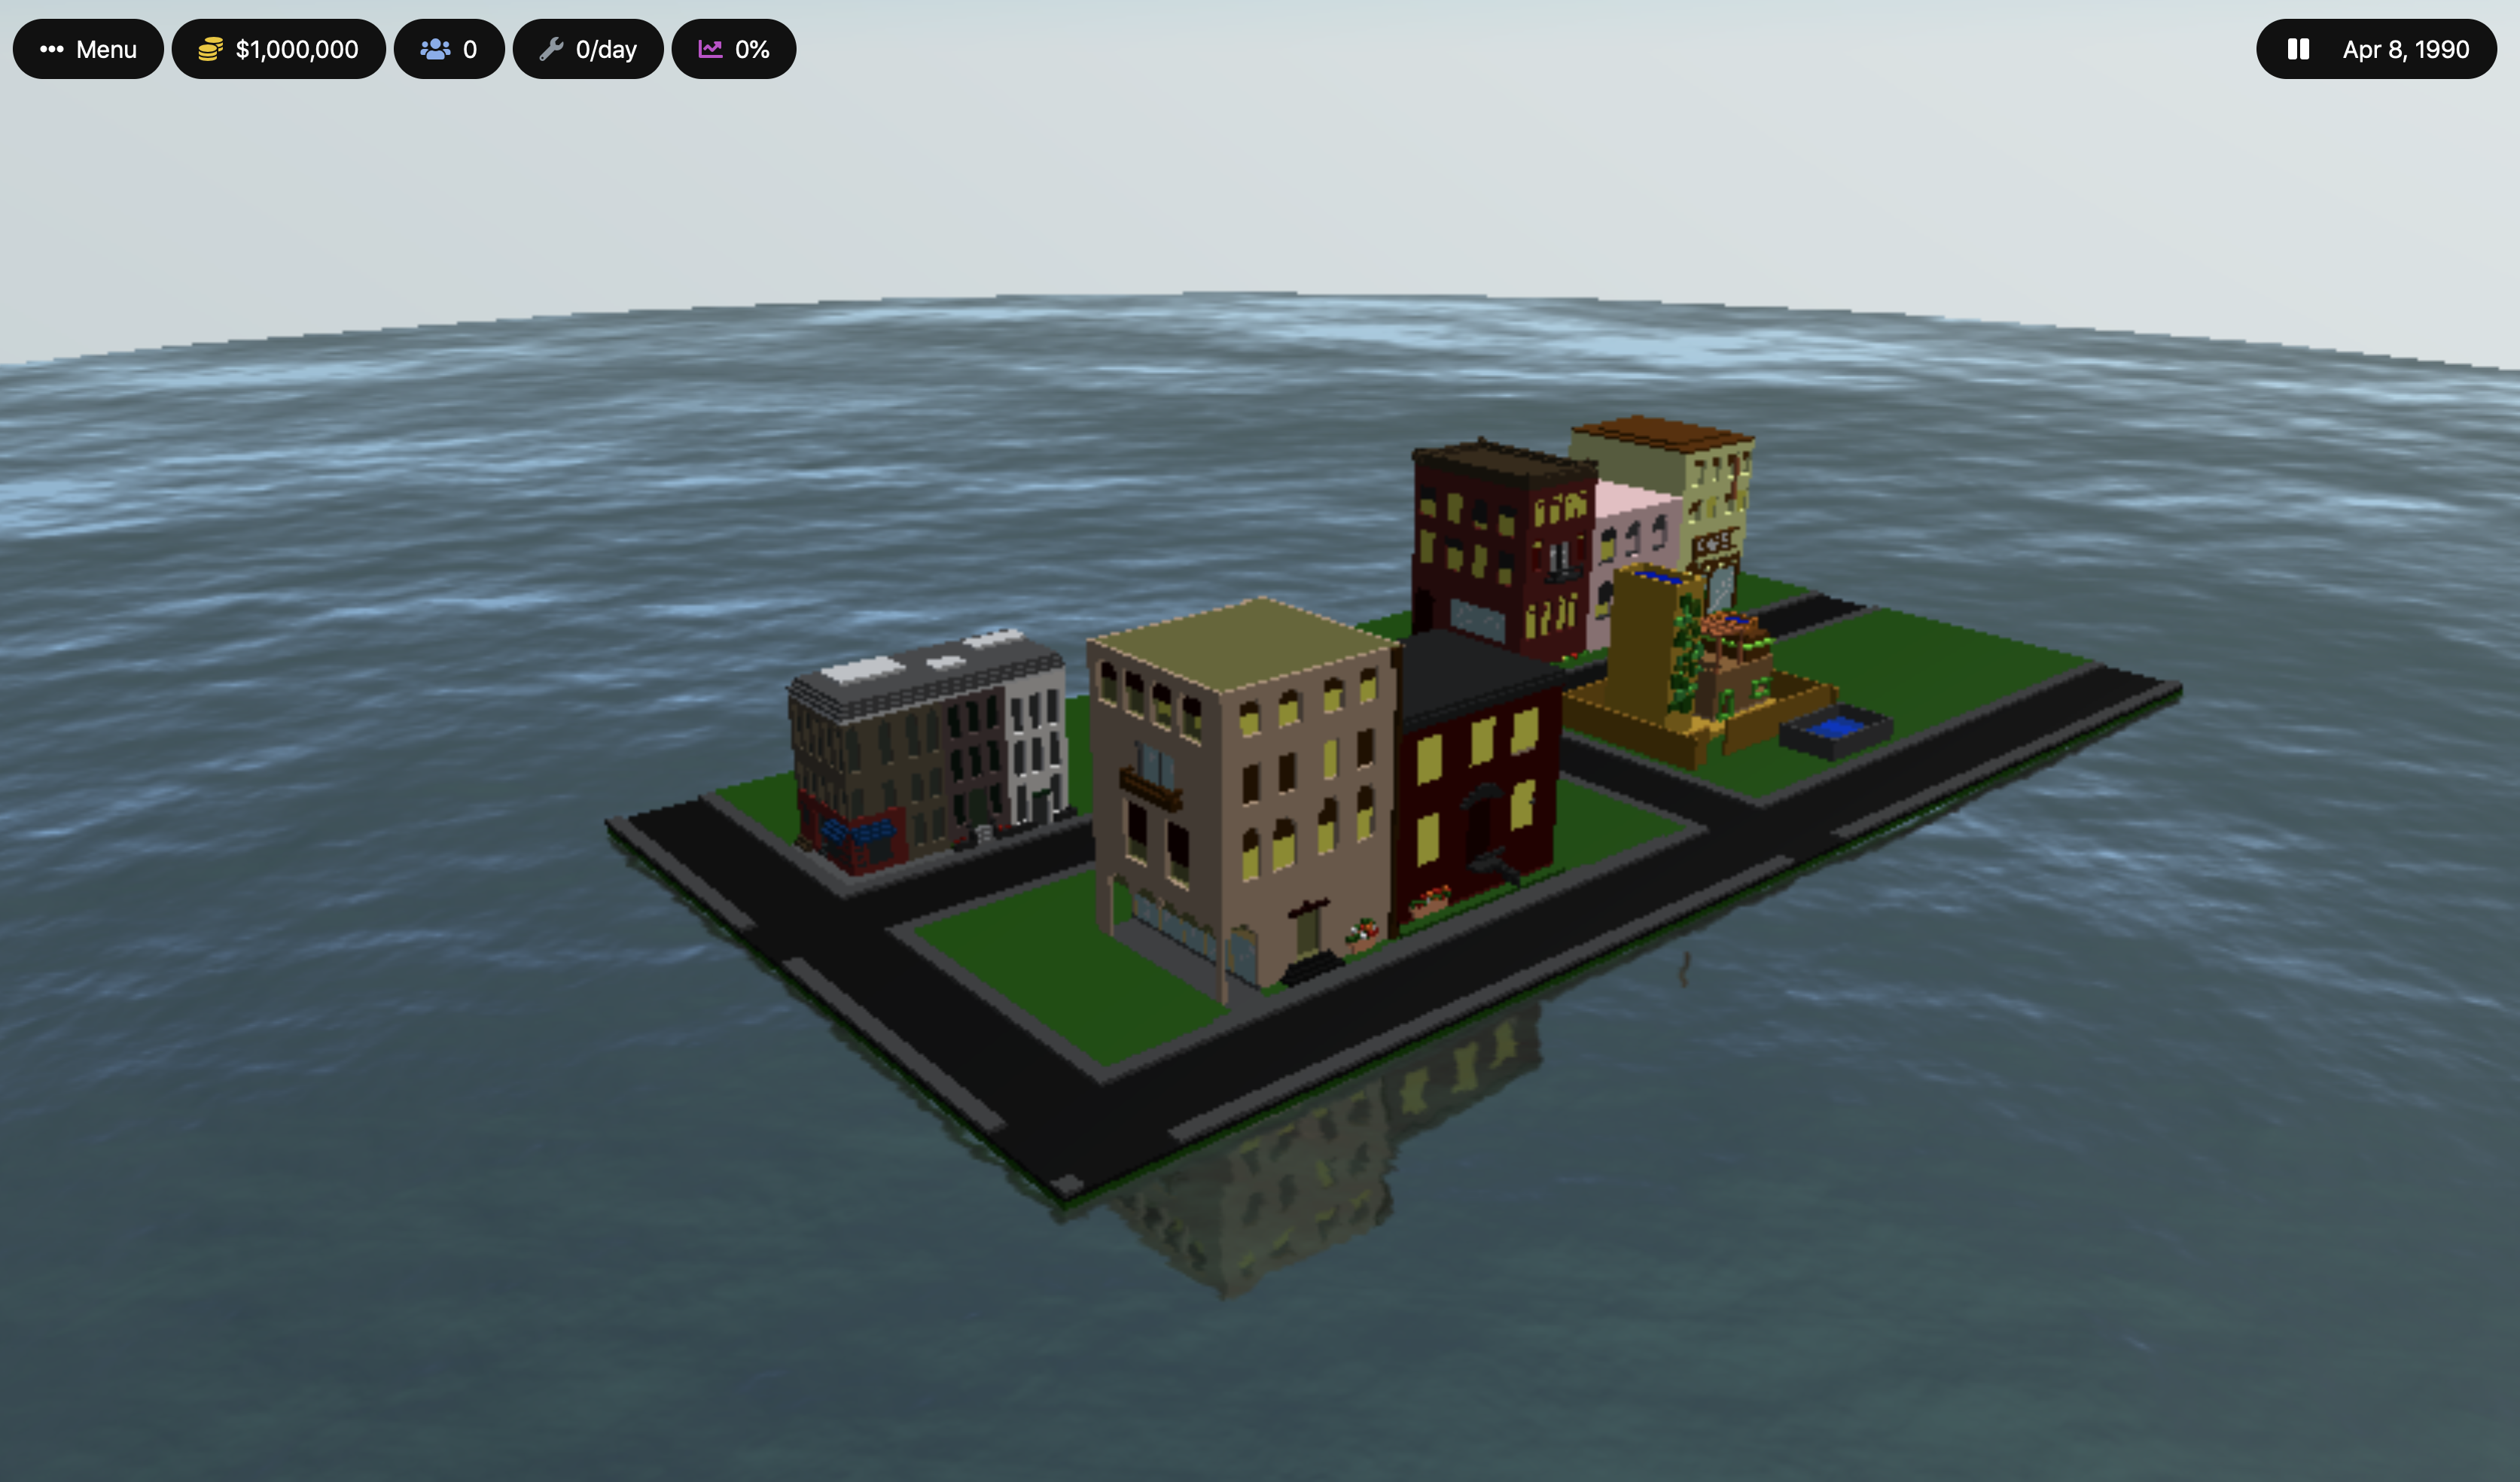
\includegraphics[scale=0.22]{images/screenshot-map.png}
    \caption{Capitalism X Map Concept}
    \label{fig:map}
\end{figure}



\chapter{How to Play Capitalism X}
\label{cha:howtoplay}

\section{Getting Started with Capitalism X}
%Steffen, Nike Halbe Seite\\

Are you ready to get started? If yes, enter the following URL to the Google Chrome browser and start your first game of Capitalism X: \\
\texttt{https://swaldmann.github.io/CapitalismX}.
However, it is advisable to have a look at the limitations as described in chapter \ref{sub:currentState} first. Now you have the possibility to start a new game or load an existing game and start right away where to took off earlier. 

It is recommended to have a look at the following tutorial if you have not played Capitalism X before. Also, it might be very helpful to read this game manual, as it gives you a couple of hints about how to handle some situations. The manual at hand gives you an overview about the different buildings and views in the game. Also, it provides you with step-by-step instructions on how to perform the most important activities.

\section{Interface and Features}
The end-to-end process of the game consists out of three major steps: hire employees, buy machines, introduce and produce products. These activities have to be performed in order to earn money. The following chapters give you insights about how to perform the mentioned process steps.

\subsection{Controls}  
The main screen after starting a new game or loading a game in Capitalism X is an interactive map of all functional and non-functional buildings, which can be found in \ref{SettingStory}. In the government building you can choose and hire lobbyists, whereas in the job center you can select and hire your employees. The functional building of the harbour is your procurement area, where you can buy the components needed in order to manufacture products. Last but not least, you also have some competitors. By visiting the competitor buildings you will get insights about their market shares.

You can adapt settings or get an overview about the department specific performance by either clicking on the functional buildings or using the navigation bar at the top of the screen. The navigation bar can be seen as your headquarters, as all internal departments of your company can be found there. The departments in the navigation bar are finance, HR, production and marketing and include links to all other functionalities in the game. 
\begin{figure} [!htbp]
    \centering
    
\includegraphics [width=\textwidth]{images/navigationBar.png}
    \caption{Navigation Bar}
    \label{fig:navigationBar}
\end{figure} The detailed actions and settings are described in later chapters, but in the following you get an overview about the different actions that you can do by using the navigation bar.

In the HR view, you can adapt all settings regarding human resources and employees, such as hiring and firing employees. Also you get insights about the employee satisfaction and other key figures. For more information about the HR view, please go to chapter \ref{HR_manual}.
The finance view, provides you with an overview about the financial situation of the company, by giving you dashboard consisting of different performance indicators, such as cashflow and net worth of company. Also, you might take action on financial topics, such as taking a loan from the bank. You can find details in chapter \ref{finance_manual}.
Next, you can procure, produce and sell goods and equipment in the production view. For more insights on procurement, production, selling, and logistics, please take a look at chapter \ref{production_manual}. 
Last but not least, you can visit the marketing area, where you can start marketing campaigns, start market research activities or commission consulting companies. You can find more information in chapter \ref{marketing_manual}.

Throughout the game, time passes starting from January 1st, 1990 on. You can see this time at the top right corner of the screen and can be seen in picture \ref{fig:time}.
\begin{figure} [!htbp]
    \centering
    
\includegraphics{images/time.png}
    \caption{Time in Capitalism X}
    \label{fig:time}
\end{figure}
Next to the time box, there is a little "pause" sign, where you can pause the time in case you want to adapt some settings and do not want the time to elapse before you finished your adaptations.

Apart from that, at the bottom of the screen you can find a news ticker banner, that gives you subtle hints about possible settings to adapt. A proper example here would be  If warehouses are full, no more products can be stored for sale. In Capitalism X some unexpected incidents may happen to your company or to the environment, for example it could happen that an earthquake destroys part of your production facility or that a sudden hacker attack is going to steal sensitive data from you. In these cases, urgent intervention from you is needed! Therefore, a pop-up window will open, where instant decisions have to be taken. It is absolutely not recommended to ignore such pop-up windows, because an omitted action is highly probable to cause your company huge damage.

% How to Finance
\subsection{Financials}
Nike, Salih\\

Financial actions occur throughout the whole company as it can be seen as the engine that keeps the whole company running. The success of your company depends on your financial strength. A healthy balance between income and expenses ensures the competitiveness of your company. Therefore, the organization of finances is an essential part of management. The question of raising capital must be defined in order to have a good mix between debt and equity.\\

You can choose from a variety of ways to raise capital. A distinction is made between internal and external financing vs. equity and debt financing.
Financing from within the business is the internal financing, while financing from organizations outside the company is called external financing. Equity financing occurs, when raising money in exchange for a share of ownership in the business whereas borrowing money, that must be repaid over a period of time, is the debt financing. In CapitalismX the main source of capital should be the internal financing from your goods sold. However, also external financing in the form of debt financing is possible. In this case, you as the CEO have the possibility to loan money from the bank. (add some references). \\

 The entry point for the financial actions is the finance dashboard. You may find it by clicking on the finance button [screenshot] from the navigation bar at the top left. The dashboard gives you a detailed overview about several areas at first glance:
\begin{itemize}
    \item Cashflow, which is basically your profit and loss statement displaying revenues, expenses, and profit on a quarterly basis.
    \item Statistics, showing the development of salaries and total sales in visualized graphs.
    \item Company information, divided into cash, assets, liabilities and company net worth. This view gives you information about the current liquidity of your company.
    \item Bank, providing the possibility to request a loan from the bank or to get an overview about current loans.
    \item Investments, where the you might invest some money in the stock market.
    \item Product performance, giving an overview about product specific key performance indicators, such as the sum of material costs per product.
\end{itemize}
[SCREENSHOT IN APPENDIX WITH REFERENCE???] The cashflow, statistics, company information and product performance are solely descriptive information, that is generated from the actual settings defined by you as the player or by your company’s performance. The goal of these areas is to provide an overview about the general financial performance status of the company and should give you hints about adapting some parameters. [DESCRIBE MORE IN DETAIL, e.g. company net worth is ebit with added loans and substracted taxes and interests i.e. most important financial key figure bla???] However, the bank and investments area require input from your side, which you can provide as needed. \\

While you are building an empire, it can happen that you suffer financial bottlenecks, but also that you perform better than expected. In order to avoid or react to bottlenecks you might want to make use of debt financing, hence you have the possibility to borrow money from your bank. If you are performing very well, you might want to invest some CapCoins in the stock market.\\

You can visit the bank using the Finance Dashboard. Here you can request credits, but you can also see an overview of credits you have already received.
The list of credits you have already received gives you a detailed overview of repayments. Here you will find a list of the loan amount, the monthly or annual interest and retirement as well as your remaining debt. The agreed repayment plan is automatically booked from your bank account in accordance with the previously determined conditions.
If you are in financial trouble or planning a major investment, you can request a loan from your bank. The bank will provide you with a choice of short, medium, and long term loans, which you can accept or decline. You should note that the bank always uses your company value as a basis for assessment and takes this into account when granting loans or reject your request. \\

Apart from that, you might invest some money into innovations on the stock market, which is similar to the well-known DAX stock market. As this may be a risky undertaking, due to the regular oscillations on this market, a good idea is to spend only a reasonable amount of money there. \\

Pricing and selling of goods might appear as a financial task to you, but in fact, you will find information about these topics in the manufacturing view.\\ 

%Pricing and selling -- put into production view \\
%pricing: user sees cumulated costs per product incl. employee costs (LIVJAS formel) and may decide on a profit margin to add to the costs. He gets some hints and the value addded as percent. (explain UI part in 4.x chapter).


 

%How to HR
\subsection{HR} 
\label{HR_manual}
%Maike and Philipp
One of the most critical resources that a company needs in order to get a competitive advantage, are the human resources (HR).
The goal of the HR department is to maximize the employee performance in order to support the vision of the company. The HR department has many responsibilities. This includes personnel planning, recruitment, compensation and benefits, training and development and performance management.

Personnel planning contains the determination of employee requirements, including number (capacity per head), quality, time / duration, location (domestic / foreign, location, department, cost center) and costs. Steps of recruitment are needs assessment, advertising, selection, negotiation and introduction / training. The aim is to achieve a cost-effective and fast procurement of the desired employees, which involves identifying and hiring high-performing employees. 

Compensation and benefits means creating, managing and improving a company's compensation and performance structures. Wages and benefits are two crucial factors that ultimately determine how well your employees feel about your company and how likely they are to stay with it in the future.

Training and development includes the ability to create training programs that solve the performance problems of employees and create additional incentives for employees to improve further and thus also advance the company.

Furthermore, the development and implementation of a complete performance management and improvement process is an essential capability of a company. The design of the performance assessment process, its maintenance and the effective monitoring of its implementation represent challenging tasks for a company. 

As not all of the above mentioned tasks are suitable for a simulation game, we concentrated on some aspects which are of strategic importance.

The HR process of the CapX Game is mainly structured in three phases
\begin{enumerate}
    \item Hiring
    \item Development
    \item Motivation
\end{enumerate}

In CapX there are two types of employees of main importance: engineers and sales employees. In order to be able to produce products it is necessary to hire available engineers on the market. Moreover, to sell the produced products, sales people are needed who are responsible for the entire sales cycle of the company.

\begin{figure} [!htbp]
    \centering
    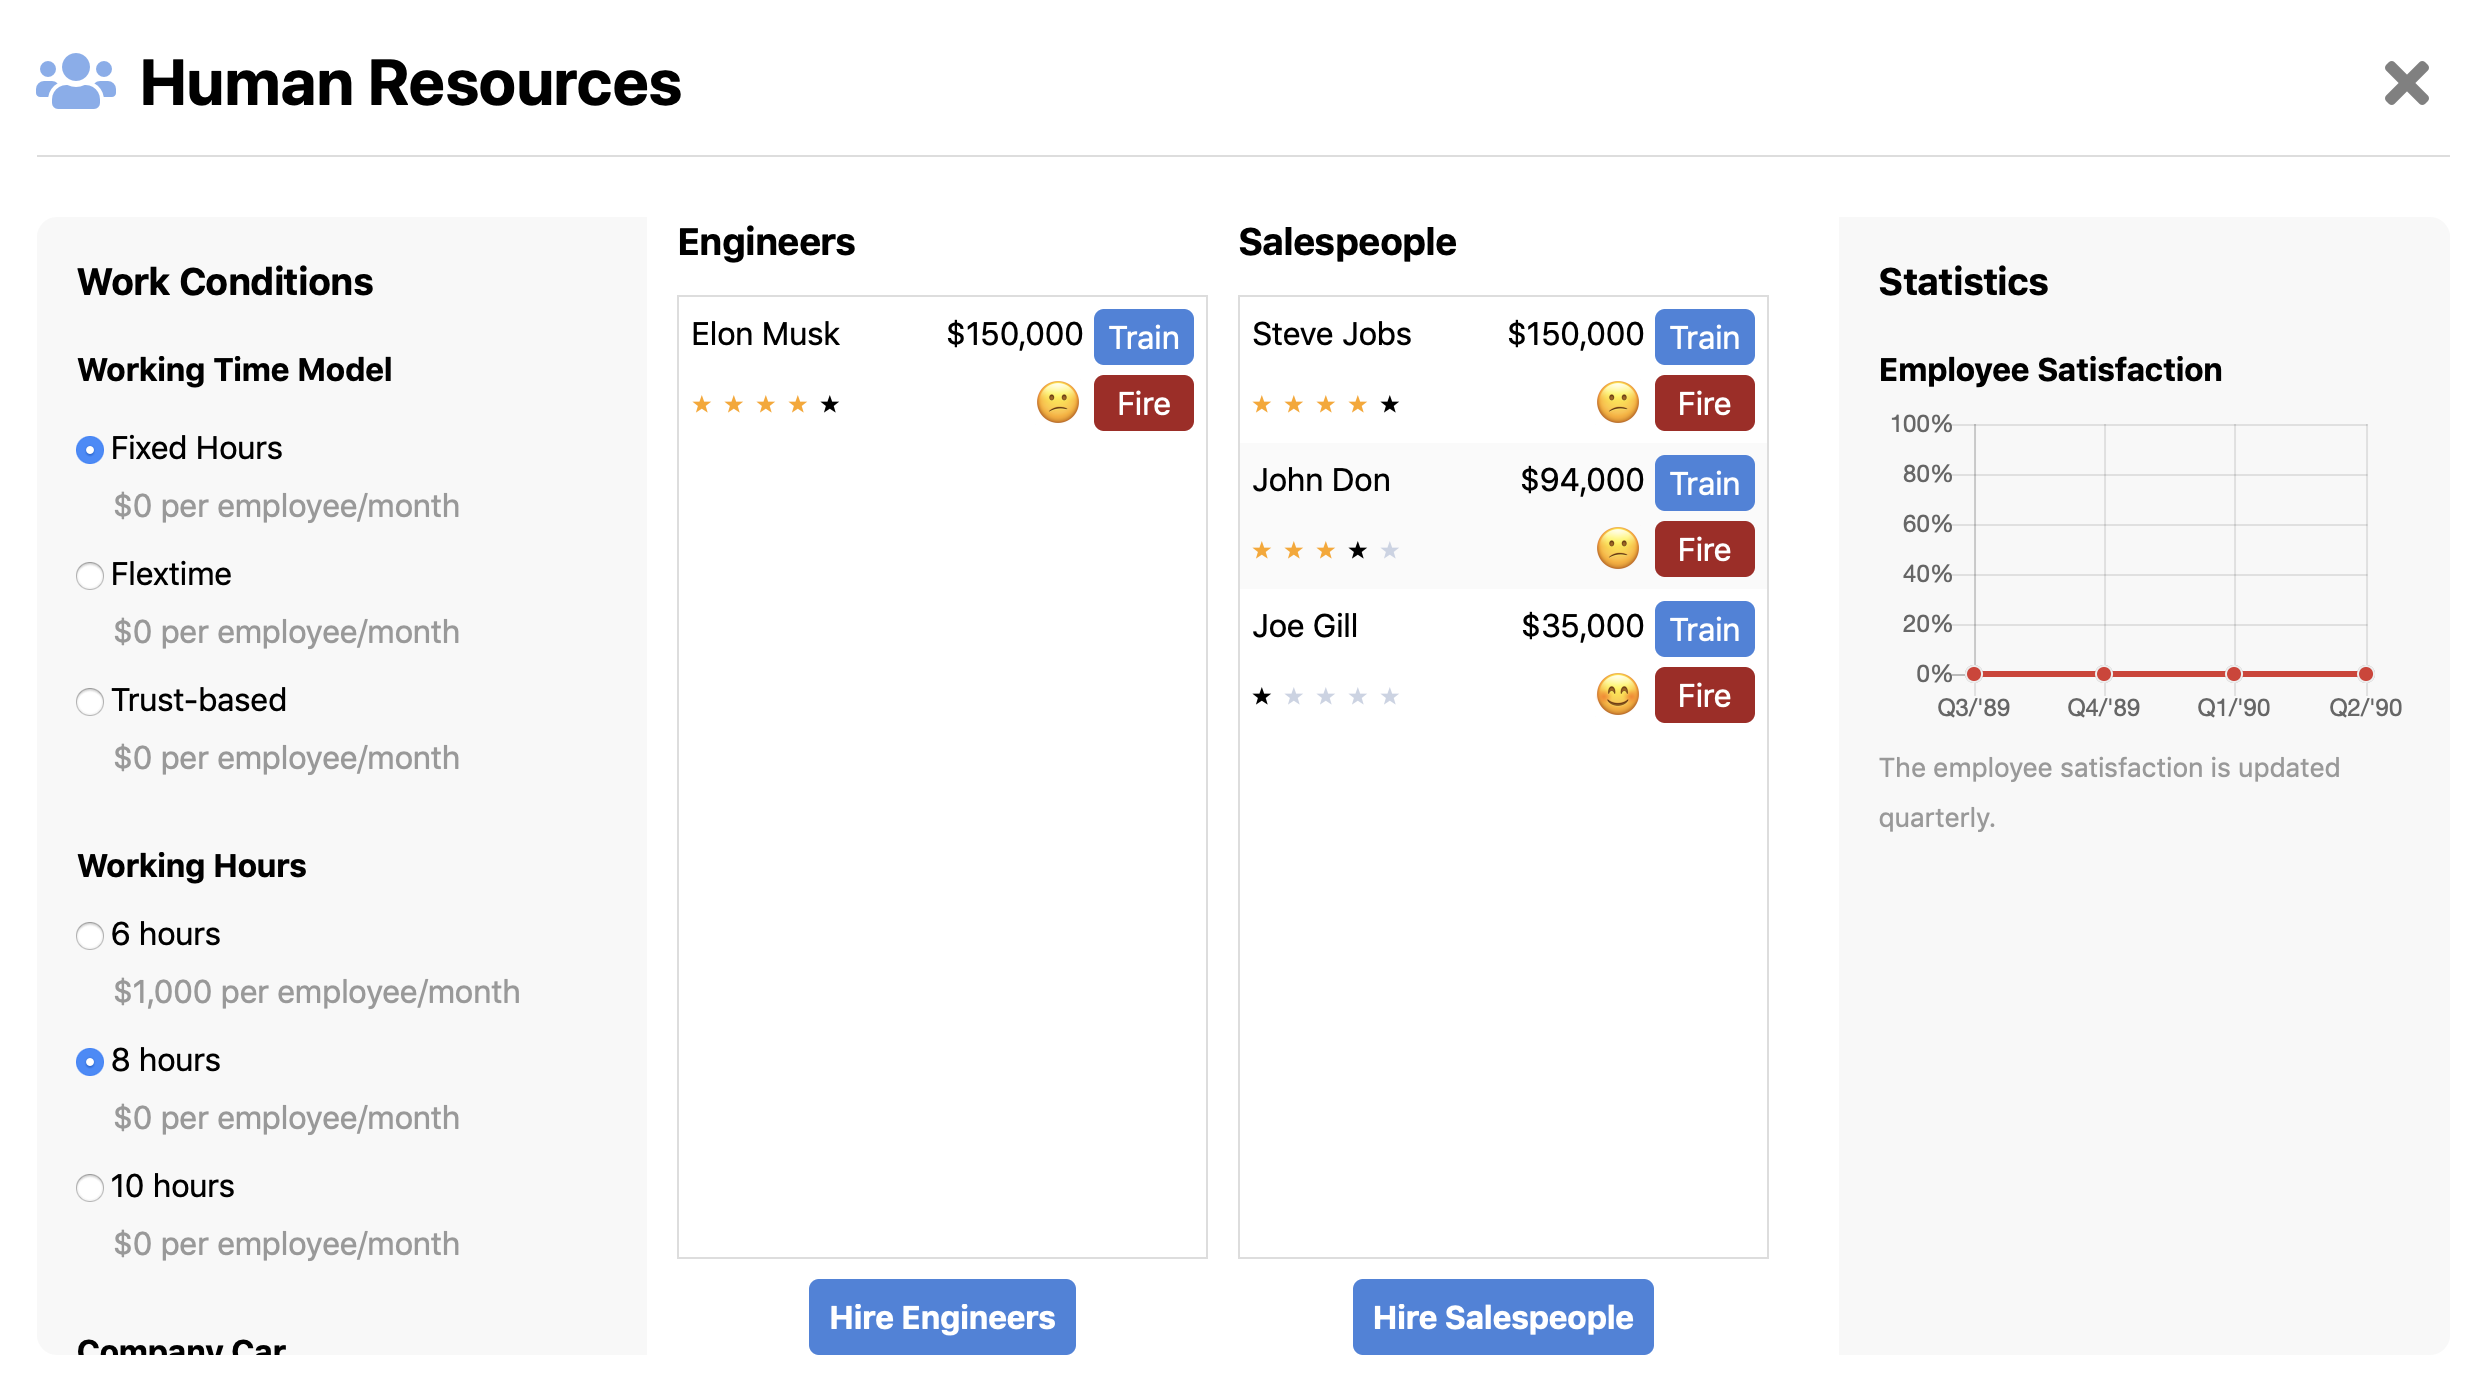
\includegraphics [width=\textwidth]{HR/hr_view.png}
    \caption{HR view}
    \label{fig:navigationBar}
\end{figure}

The HR view allows you to see the available employees on the market per department. For each employee you will see their names, their skilllevel (indicated by stars) and their salary demand. Depending on your own HR strategy you will have to decide whom to hire. Be advised that hiring and firing employees is not a one time activity but rather a constant task. Your strategy needs to be executed throughout the entire game.

After you made your initial first decision about your workforce you can start the workforce development by choosing the necessary training for your employees. In order to develop, grow and gain new knowledge, your employees are required to be trained continuously. Lifelong learning is an essential part of every HR strategy. By clicking the train button you can train single employees, but also entire teams. Make sure that you really choose a training that fits to the needs of your employees so that they can maximize their benefit from it.

The third pillar of your HR strategy is the motivation. Providing the right extrinsic motivation is necessary, so that your employees feel valued. The extrinsic motivation can be provided through the usage of benefits. On the one hand, benefits motivate employees and ensures a positive contribution to the work-life-balance, but on the other hand, of course, benefits cost money. Your task is to find the best possible balance and especially execute on your strategy. Make sure to think first, which HR strategy you have and then choose your options wisely. The benefits view is also provided in your HR view.

%How to Production
\subsection{Production}
\label{production_manual}

In our concept of CapitalismX, the production process is a grouping of various other factors. These factors are, namely: 
\begin{itemize} 
\item Products 
\item Procurement  
\item Machinery 
\item Logistics 
\item Warehousing 
\end{itemize}
You will find all of the above mentioned processes in the tabs of the Production View. Each tab contains all the respective elements, that keep the production process running.
The manufacturing process, which is the focus of this section is composed of several elements. Most of these elements will be visible to the user through the Production view accessible in the CapitalismX game settings. Furthermore these elements, will serve as variables that will interact with each other in the game mechanics, and provide the user with the appropriate indicators of performance, regarding the Production process. However other important elements will not be directly visible to the user but will serve a very important role in the game mechanics. How this occurs will be explained in chapter \ref{sec:productionSim}. \\
In this section we will explain all the different views and elements you can encounter whilst browsing the production view, with the exception of Logistics and Warehousing, which you can find in the dedicated chapter ...... \\
\subsubsection{Product View}
\label{sub:ProductView}
Now it is time to generate some revenue for your hard work! After hiring engineers, procuring the components and machinery needed, you have to decide on a market price for your respective product. In order to do so, you might go to the product view tab in the production area. There you get an overview about each product in your portfolio. [screenshot]

First, you can see the product’s name, which you can adapt in the procurement view. Second, you can enter the quantity you want to produce. Next to that, you have the amount of units in stock displayed. The amount in stock will be reduced automatically when some customer buys the respective product. This means, that only if the stock is empty, products with new components will be sold to the market. However, you can produce all the time and increase the units in stock if the market is not responding yet. 

Back to the UI: next to the units in stock you can see the cumulated product costs, which include the sum of component prices, and other fixed costs, such as electricity, and variable costs that occur during production. Based on this amount of CapCoins you might enter a market price in the next field. The respective profit margin is calculated automatically and displayed next to your defined market price. Again, market research and older sales figures may give you a hint about the reasonableness of your market price. 

With that being said, the actions you are required to take are defining the price per product in the production view. Then, as soon as you enter a quantity, the products are produced if sufficient production capacity is available. Otherwise, the products are manufactured according to the FIFO principle. After production, the products are available for purchase by your customers on the market.

\subsubsection{Procurement View}
\label{sub:ProcurementView}
In order to start manufacturing or retailing goods, you need to procure the components necessary. First, you need to choose a suitable product portfolio for you. In order to do so, please go to the production area and select the procurement tab. There you have the possibility to add a new product to your portfolio. In the beginning, it is reasonable to start with a smaller product portfolio. [SCREENSHOT] In later stages of the game however, it might be interesting to test out the production and sale of different products, and maybe even different version of products, for example selling a high-quality, high-priced smartphone and to compare it to selling a low-quality, low-priced smartphone. Insights of such experiments might be derived from market research, sales figures, etc.

Also, you have an overview about the components the engineers need in order to manufacture a specific product. Some might be locked at the beginning and will be unlocked in due time. When clicking on a component, an overlay opens where you have the possibility to select the component from three different suppliers. [SCREENSHOT]. There are several features that help you decide which supplier to choose: the price, the eco-index and the quality index. The price varies, depending on the supplier. Next, the eco-index is a measure that defines a supplier’s ecological footprint, influenced by their logistics, sustainability in production, ecological footprint of their suppliers, and so on. This means, the components you choose might also have an influence on your company’s eco-index. Third, the quality index gives you insights about the component’s quality, so the higher the quality index, the higher the component’s quality. Again, the component’s quality has an influence on your final product’s quality index, which you should keep in mind, when defining a product’s price.

After deciding on a component from a supplier, you need to choose the amount of components you want to purchase. For a higher amount, you might get a mass discount, but beware --  buying more components than you manufacture to products may lead to higher warehousing costs. 


\subsubsection{Machinery view} 
\label{sub:MachineryView}
Let us continue with the Machinery view, which indicates a snapshot of the current status of the company's machines. Their number and overall capacity, can be found on the left side of the tab. When looking at the right side of the tab you can get a more in depth perspective of each machine. The current capacity is a value that shows the user the maximum amount of products that the machine can produce in a day. 

 In the list of the individual machines, it will also be possible to maintain, upgrade and sell individual machines. The maintain and upgrade options improve the selected machinery state or in other words its production technology. 
The user will also be presented with the opportunity to buy several machinery, which will all be of the same type. In the production process a machine can produce all types of products, meaning production machinery are not product specific and vice-versa. This decision has been made due to simplification of the entire production process simulation. The differences these machinery will have regard their producing capacity, and their production technology level. 

The production technology level is a value which shows the current state of a particular machinery. For this measure we developed a scale similar to the company’s general Eco-Index, but at the same time different, as it is adapted to the Production machinery.  This scale has a range from $1$ to $5$, where $1$ is a deprecated machine, and $5$ is a brand new machine. When a machine is bought it has a certain value for the technology scale, which is related closely to the price the users pay. This is also presented in Table \ref{table:my-label}. 

The overview of this logic is represented in the actual Production view by a pie chart. We chose the pie chart as it permits a visual check of the reasonableness of the overall machine state and the differences between several states. Moreover, it is visually simpler than other types of graphs.
 The expanded logic behind the technology level can be found in the production simulation, in chapter \ref{sec:productionSim}.
 
Apart from these options, there is also the possibility to sell a machine. The selling price will be determined by the game mechanics and cannot be altered by the user. This amount will be based on the capacity of the machine and its production technology level.

In the machinery view, there are also some investments that you can make. In order to invest in R\&D, System Security or Process Automation, you have to input the amount of CapCoins you want to invest. The amount you can input is either $100cc,500cc,1000cc,1500cc,2000cc$. You will have to contemplate how and what do these investment options affect, to be able to call yourself a CapitalismX pro.

\subsubsection{Performance Metrics}
This section will give you a short introduction to all the metrics that we have selected to display in the Production View. Do not be intimidated by the multiple graphs and parameters, as these metrics are your friends. They will show you everything that is happening in production, why is it happening and how well is it going. All you have to do is figure out how to keep those levels soaring. 

The first performance metric you will encounter is manufacture efficiency (ME). This metric will show you how efficiently you are using your machines, in terms of units produced.
Just below manufacture efficiency you will see production process productivity(PPP). This measure is similar to ME, because it measures efficiency, but in the same time different as it encompasses the efficiency of the entire production process. 

You will want to keep an eye on product quality, as this value is one of the most important in our simulation. It is influenced by a variety of factors from different departments, and in order to increase your product quality you have to discover and  boost them all.

The last performance metric is production performance, this measure will give you an overall impression of the performance of the production process.

Every metric will be generated by the game and you can not influence them directly. Step by step you will come to an understanding of how different elements in the game affect these metrics directly or indirectly.

\subsubsection{Logistic and Warehousing}
%Janine
Now that your products have been produced, it's time to take care of their delivery, as the products sold must somehow reach your customers. You can control the delivery and storage of your products in the logistics view. 
All products you produce are temporarily stored in your warehouses before they are delivered. You can either build warehouses by yourself or rent them, just as you like. If you decide to build a warehouse you can sell it later at its current value, rental contracts can be cancelled at any time. Per camp you have of course certain maintenance costs like for example electricity and also the storage of products which were not sold directly on the day of their production cause costs.

You can either arrange the delivery of your products via your own logistics fleet, outsource it to an external logistics company or combine these two options. You can easily buy trucks for your own fleet, but each truck has certain characteristics that affect the overall logistics of your company. Like the warehouses, your trucks have monthly maintenance costs. In addition, there are certain delivery costs per product. If you notice that your logistics fleet is too large and you don't need some trucks at all, you can simply sell them again at their remaining value.

Just like the trucks, in the logistics view you can also view the external logistics partners, hire them and, if desired, discharge them again. Every partner company has certain characteristics, which also affect your logistics. If you decide to work with a partner, you sign a contract, which regulates the monthly costs for the general provision of the service and the costs incurred for each package delivered. 


%How to Marketing
\subsection{Marketing} \label{marketing_manual}

\gls{CSR} %Corporate Social Responsibility

%Janine
Now that you have already hired employees, bought components, manufactured products and also delivered them, you have probably wondered how to advertise them and how to communicate with your customers. It's easy, just switch to the marketing view. This includes internal communication, external communication, legal topics and market research.

So you can offer your employees additional courses that go beyond their actual work activities, such as stress management or teamwork to name just a few.

If you want to advertise products or put your company in the right light, you can do this through campaigns. Possible campaigns are: promote a green image, CSR campaign, promoting the company itself, and many more.

If you want to communicate certain messages to your customers you can do so with the help of the press releases. For example, you can assure your customers that their data will be handled with care in your company or apologize for delayed deliveries if this should happen.

In addition to communicating with the population, you can also conduct surveys among them. Click on the 'Conduct Research' button to select the report you want at the end. You have the possibility to carry out the market research yourself or to commission a market research institute with it. If you do it yourself, you can even choose how the actual customer survey is to be conducted. For example, an oral survey is more expensive than an online one, but yields immediate results.  By contrast, an online survey takes longer, which can cause the data to be slightly out of date.

You can basically choose between three reports, a price sensitivity analysis, a customer satisfaction analysis and an overview of various market statistics. The price sensitivity analysis shows you how the buying behaviour of your customers changes when you increase or decrease the price. All other influencing factors are kept constant. The customer satisfaction analysis tells you how satisfied your customers are with your individual products as well as with your company as a whole. The general market analysis shows you a series of market key figures for your products at a glance. 

If you feel that you need help managing your business, or if you just want to be more successful, you can hire either a lobbyist or a business consultancy. The lobbyist will positively help you with the government and try to support you in achieving your goals. 
A management consultancy will take a closer look at your business and try to find areas where you can improve your performance in order to become even more successful.

\section{Product Portfolio and Challenges}

\subsection{Choose the Product Portfolio}
\label{sub:portfolio}
%Nike - Description of products 

You as the CEO decide which products you want to offer. In Capitalism X, there are two different types of products. Those two different groups are manufactured goods firstly and resale products secondly. Resell products are simply bought as a whole and resold under the company brand.

To start with the resale products, consisting of two different sub-groups of products: the mass storage devices and the movie playback devices. As the products evolve over the time frame of the game, the scope of the single product group also changes. Mass storage devices will evolve, given a decent investment to innovate, from CD over DVD to Blu-Ray, from small SD cards to SD cards with very large memory, and from USB sticks with small memory and in simple versions to evolved versions with large memory. Movie playback devices may evolve from simple video recorders for recording tapes to DVD and Blu-Ray player, that even can become smart.

The larger part of the product portfolio consists of the manufactured goods. To produce those, you have to slip into the role of a strategic head of manufacturing and you have to take care about the education and satisfaction of employees in order to provide a high manufacturing and therefore also high product quality; about the procurement of components and warehousing of products; and so on.
The manufactured goods are divided into four product sub-groups, which are notebooks, phones, Game Boys, and televisions. 

Contrary to resale products, the manufactured products consist of single components, that you have to procure in the procurement view. Also, you need engineers in order to aggregate the components to products. As described in section \ref{HR_manual}, the education and skills of the engineers influence the quality of the product. Other than that, the product quality is also determined on the component's age, meaning the duration a specific component is available on the market. Another difference to the resale products is, that the manufactured product's evolution is depicted by different levels, meaning that a notebook always stays a notebook, but it surely evolves to a higher performing version. To put it into a nutshell, you must continuously innovate and invest in new components, skilled engineers, and procurement of components in order to achieve the best competitive products. 

Apart from that, you have the possibility to produce more than one product from a product sub-group, which offers various strategic advantages. For example, it is possible to produce two different phones at the same time, to test out different features and product strategies in the market. Phone A could be a very basic, simple phone, suitable for basic tasks like phone calls, messages, emails, surfing in the web. Obviously, Phone A would have a rather cheap price, but also the components do not need to be the latest state of the art tech. Phone B on the other side, could be a very advanced hence expensive phone, including a high resolution camera, high-speed internet connectivity and a fast CPU.

\subsection{Challenges and Opportunities}

Planning plays an essential part in business, but not everything can be foreseen. Companies and their executives must deal with uncertainty. Let's imagine that you just packed your bags for holiday and it gets lost at the airport. Did you consider this scenario before it happened? Running a business is similar: You can cover many scenarios and possibilities, but not every possible aspect. Therefore the game includes challenges and opportunities that are out of reach. Some of them are the result of bad management, some are rewarding. Some are influenced by your actions as a player, others come around occasionally. It is clear that if employees are paid to low, they will decide to go on strike. In contrast, an earthquake may come without warning. 

Their effects become visible via various indicators, like financial figures, capacity of warehouses or customer satisfaction. An immediate response is necessary to minimize negative consequences. Or to grab the chance when it is offered. And of course, a 'just straightforward' course of the game would be boring after some playtime. 

\chapter{Game Mechanics and Prototype}
\label{cha:alg}

\section{Overview of Game Mechanics} 
\label{sec:link}

A functioning business simulation requires that all mechanics play well together. A graphical representation contains all information in one place. This helps when implementing the prototype. In addition, such an overview supports the alignment of the different in-game simulations. The overall graph, which connects all simulations, is shown below in figure \ref{fig:OverallGraph}. 
It is also assumed that we can use the game time in our calculations. With $t_d$ we denote the time of elapsed days, whereas $t_y$ is the number of years elapsed. The game time starts on January 1st, 1990. 

\begin{figure}[H]
    \centering
    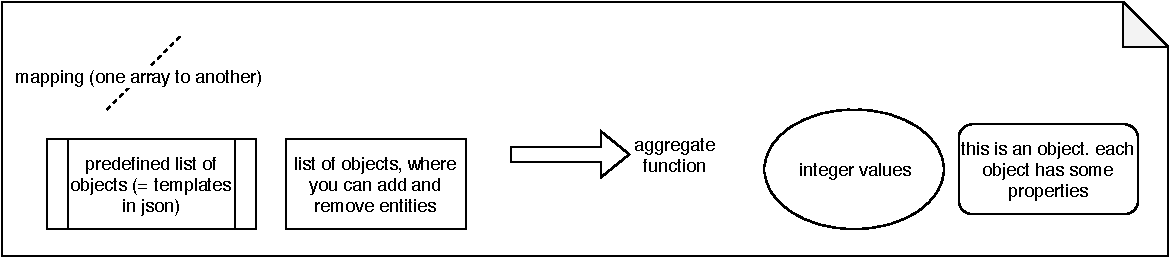
\includegraphics[width=\textwidth]{fullGraph_legend.pdf}
    \caption{Legend for the overall graph including all parts of Capitalism X}
    \label{fig:OverallGraphLegend}
\end{figure}

\begin{figure}[H]
    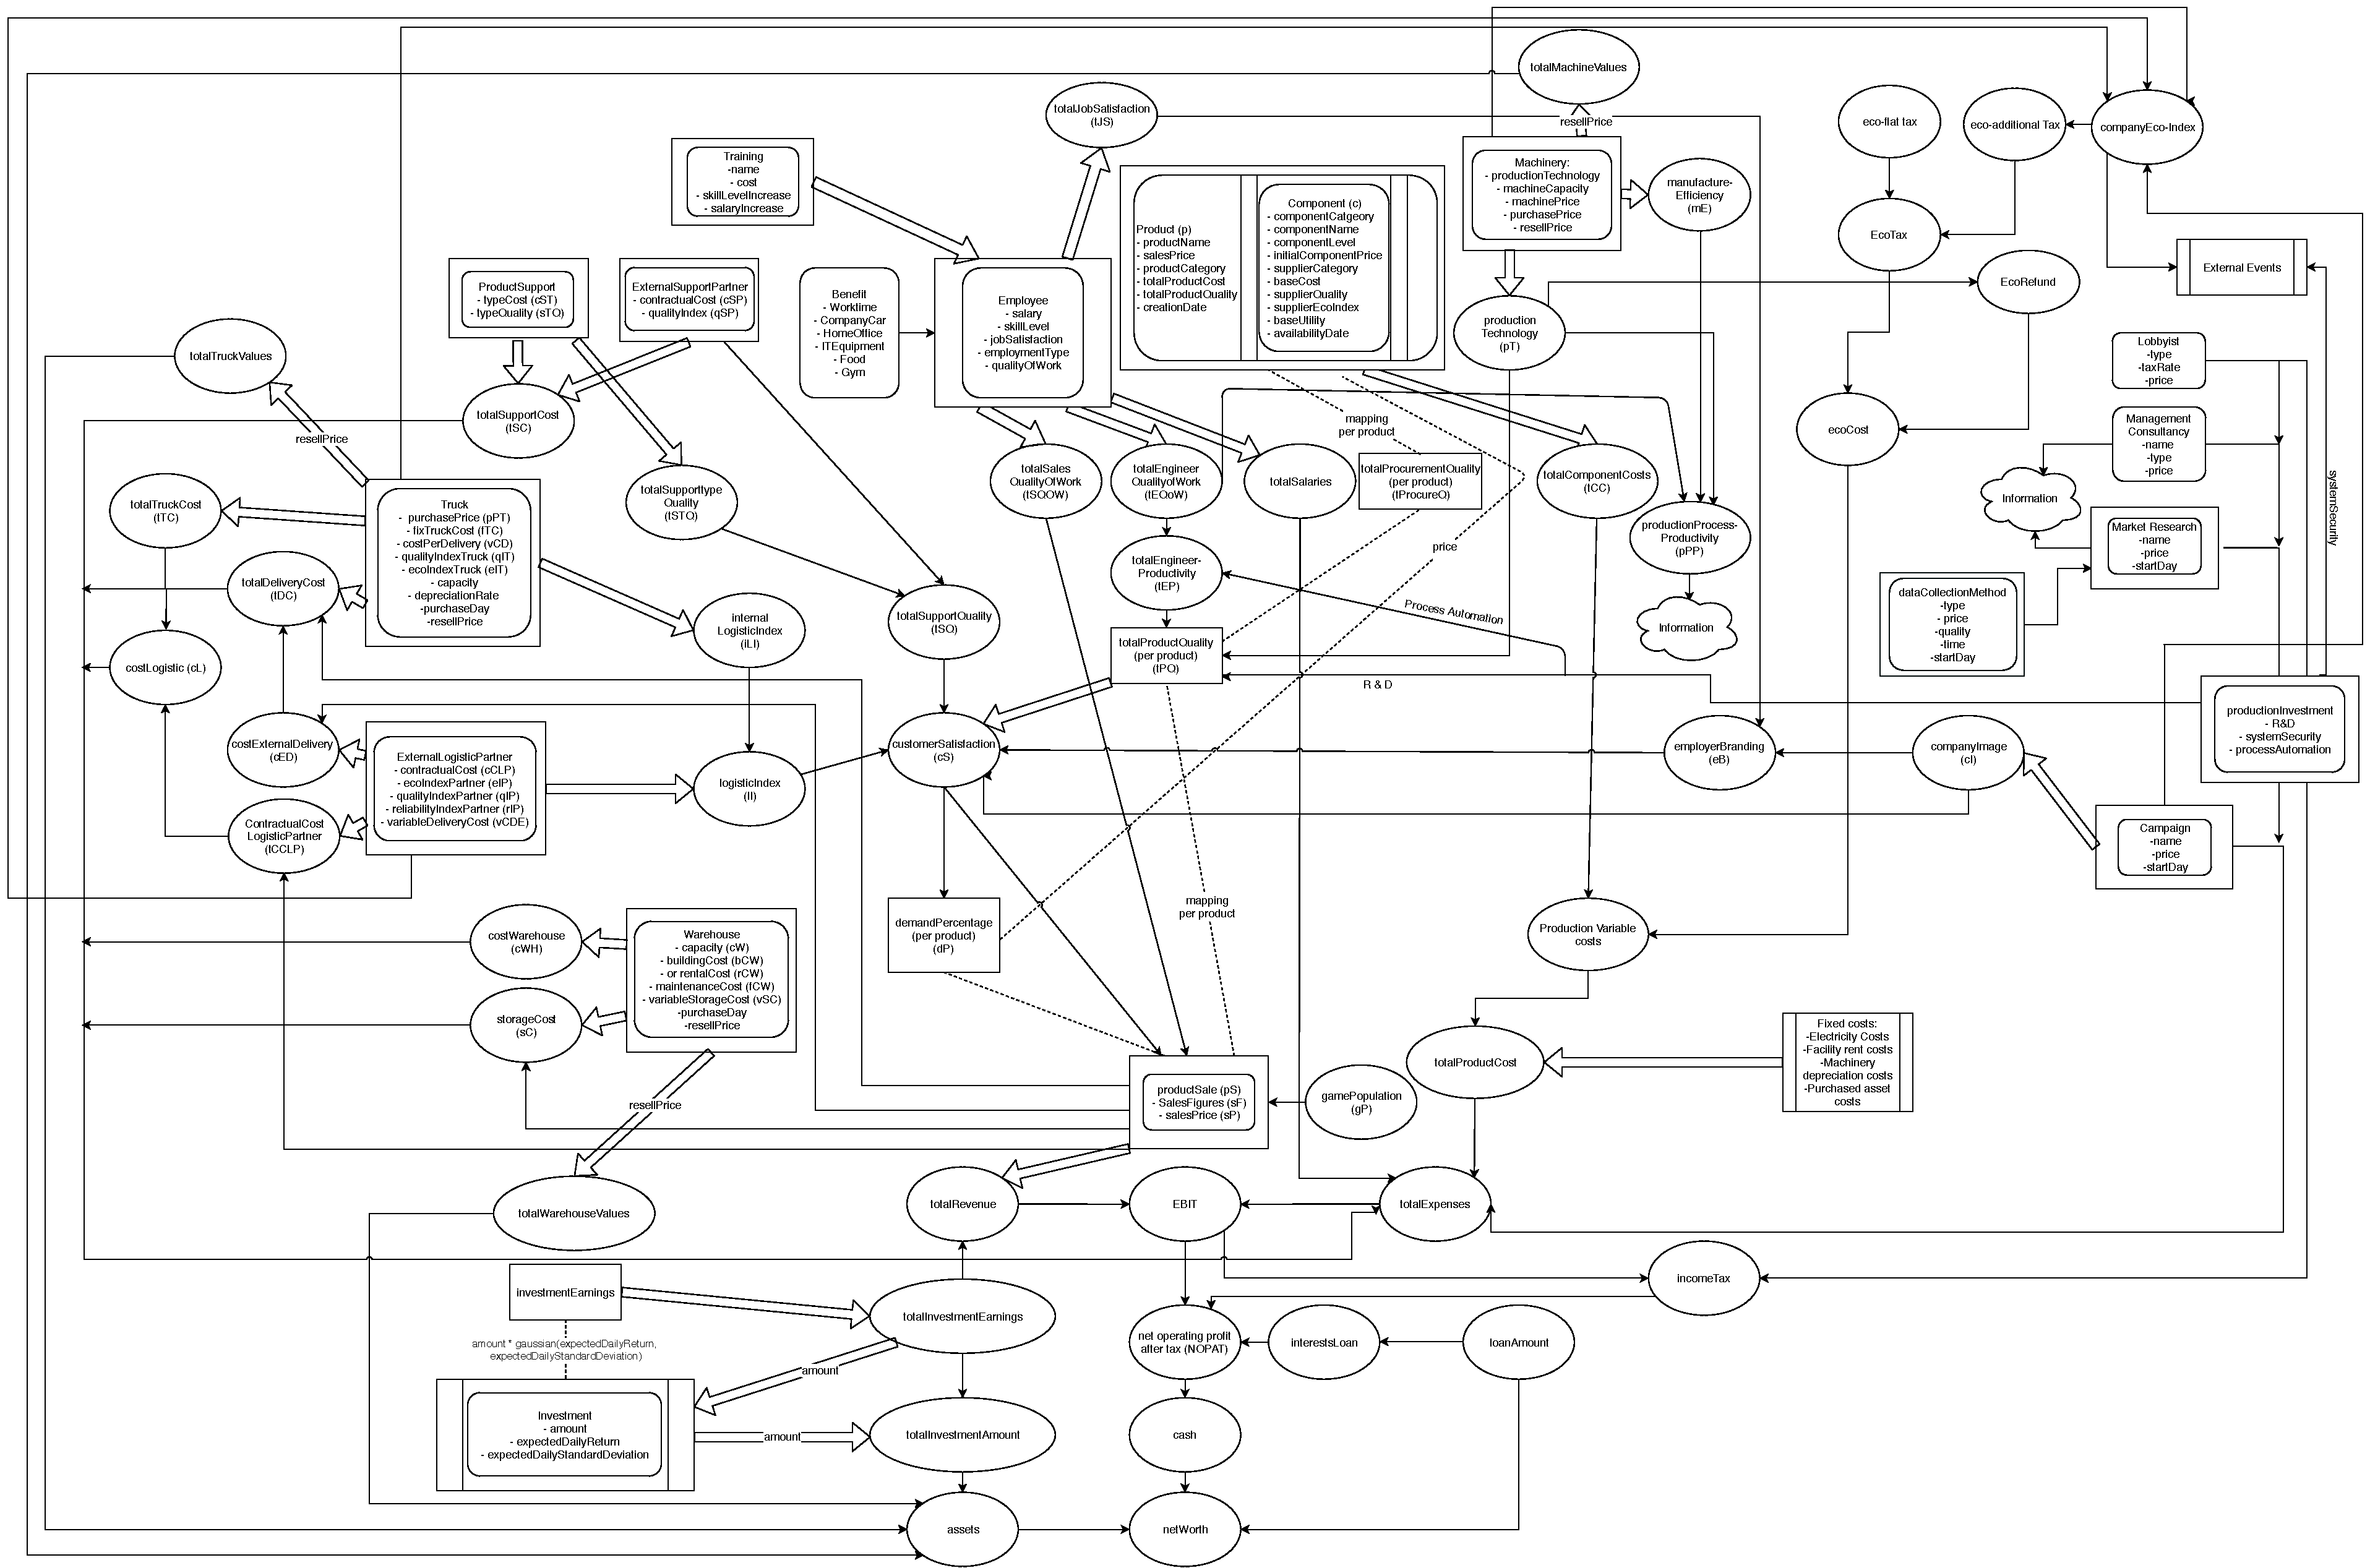
\includegraphics[angle=90, width=\textwidth]{fullGraph.pdf}
    \caption{Overall Graph including all parts of Capitalism X}
    \label{fig:OverallGraph}
\end{figure}

%HR
\section{HR Simulation}
\label{sec:HRsim}
The HR simulation handles all parts of the Human Resources Process. Two employee types have to be hired: Enigneers and Salespeople. The role of HR, Finance and Marketing is performed by the player itself, thus it is not required to hire employees in these departments for the simulation. 

\subsection{Hiring / Firing}
The HR process starts with hiring human resources. Therefore, available engineers and salespeople need to be chosen from the market. Each employee has a requested salary. Moreover, hiring and also firing of employees is associated with cost of 5000 CapCoins. \cite{recruiterbox}

\subsection{Salary}
Salaries are an important factor in the HR process. In order to make the simulation as realistic as possible, we use the following salaries which are derived from a salary-list of a real world IT company. The salaries of available employees are randomized value out of the corresponding salary-range entry in table \ref{tab:Salaries}

\begin{table}
    \centering
\begin{tabular}{c|c}
    \hline
     \textbf{Skilllevel} & \textbf{Salary-range in thousands CC} \\
     \hline \hline
     0-20 & 38-45  \\
     21-40 & 45-55 \\
     41-60 & 55-70  \\
     61-80 & 70-100  \\
     81-100 & 100-150  \\
     \hline

\end{tabular}
\caption{Salaries}
    \label{tab:Salaries}
\end{table}

\subsection{Key Performance Indicators}
\label{sub:KPI}
\subsubsection{Job Satisfaction}
The job satisfaction is an essential part of a Key Performance Indicator framework in order to measure the management quality of the player. Many different parts in the cooperation depend on the job satisfaction of employees, thus, in order to increase the performance, managers need to make sure that the satisfaction of their employees is constantly high. \cite{KOYS}

The job satisfaction is such an important factor due to the fact that the employer branding is influenced by it. This is critical as the employer branding has a huge impact on how the company is perceived on the markets by potential employees but also by customers and suppliers. Moreover, the employer branding is also influenced by the general company image and can be influenced through marketing and PR activities. 

The success of a company highly depends on the ability of attracting the best people. The ease of recruitment is highly dependent on the job satisfaction of the employees. Extrinsic motivation needs to be provided to attract employees in case the job satisfaction and by this the employer branding are low. A low job satisfaction makes it necessary to pay higher salaries. Not only the recruiting of employees is more difficult with a lower job satisfaction but also the employee turnover is higher. A job satisfaction below 50 leads to an increase in hiring costs of 50\% which sums up to 7500 CapCoins \cite{frederiksen2016}

Different factors exist which influence the job satisfaction. \cite{Kapur} The implementation and integration of softfactors which influence the job satisfaction was not the primary goal for CapX, we concentrated on the hardfactors which include salary and paymix, worktime, the skills and education and the provided benefits by the company. 

The table \ref{tab:benefitsJSS} shows the possible influencing factors which can be chosen by the player to influence the employees job satisfaction. The monetary impact is counted in CapCoins per employee per month. 

\begin{table}
    \centering
\begin{tabular}{l|c|c}
    \hline
     \textbf{Benefit} & \textbf{Points} & \textbf{Monetary impact} \\
     \hline \hline
     \multicolumn{1}{c|}{\underline{\textbf{Salary}}} & & \\
     Salary below average & 0 &  \\
     Salary on average & 2 &  \\
     Salary above average & 4 &   \\
     \hline
     \multicolumn{1}{c|}{\underline{\textbf{Worktime}}} & & \\
     6 hours & 5 & -1000\$  \\
     8 hours & 3 & 0\$  \\
     10 hours & 0 & 0\$  \\
     \hline
     \multicolumn{1}{c|}{\underline{\textbf{Company Car}}} & & \\
     Not offered & 0 & 0\$  \\
     Medium Size & 2 & -300\$  \\
     Full Size & 4 & -600\$  \\
     \hline
     \multicolumn{1}{c|}{\underline{\textbf{Home Office (HO)}}} & & \\
     Fixed Model & 0 &   \\
     Flextime model & 1 &   \\
     Trust-based (TB) & 2 &   \\
     Trust-based (TB) + HO one time per week & 3 &   \\
     Trust-based (TB) + always HO allowed & 4 &   \\
     \hline
     \multicolumn{1}{c|}{\underline{\textbf{IT Equipment}}} & & \\
     High End & 2 & -50\$  \\
     Market Average & 0 & 0\$  \\
     \hline
     \multicolumn{1}{c|}{\underline{\textbf{Food / Coffee}}} & & \\
     Offered for free & 4 & -100\$  \\
     Employee payment & 0 & 0\$  \\
     \hline
     \multicolumn{1}{c|}{\underline{\textbf{Gym / Sports}}} & & \\
     Offered for free & 4 & -100\$  \\
     Not offered & 0 & 0\$  \\
     \hline

\end{tabular}
\caption{Benefits influencing the Job Satisfaction}
    \label{tab:benefitsJSS}
\end{table}

For each of the above mentioned categories (salary, worktime, company car, homeoffice, IT equipment, food and sports) the player needs to make a decision which benefit category to offer. The job satisfaction score can have a minimum of 0 points and a maximum of 28 points.

As this scale is too simple in order to be somehow realistic, a manipulation of the original scale is needed. The marginal impact of an additional increase of factors which lead to a higher job satisfaction decreases over time, e.g. an employee which has an above average salary, a company car, trusted based working hours and all other benefits on the highest level, would not value the additional offering of a free sports club voucher as much as an employee that has no benefits at all and gets a sports club voucher. Thus the scale of 0 - 28 was transformed to a root function.

Moreover, the job satisfaction also depends on the level of the employee. Each employee has its own specific requirements and expectations. Generally, we assume that employees with a lower skill level, are more easily satisfied than employees with a higher skilllevel. In this case the skilllevel  is used as a proxy for the expectations of an employee towards the employer. 

\begin{tikzpicture}
\begin{axis}[
    axis lines = left,
    xlabel = Original Scale (OS),
    ylabel = Job Satisfaction Score (JSS),
    grid style = dashed,
    legend pos=north west
]

\addplot [
    domain=0:28, 
    samples=28, 
    color=red,
]
{x^(1/3)* 33};
\addlegendentry{$JSS=\sqrt[3]{OS}*33$}
\end{axis}
\end{tikzpicture}

\subsubsection{Quality of Work}
The quality of work is a measure for the output quality of every process step in the corporation where an employee is involved. We are aware, that the quality of process outputs is influenced by more than the chosen factors here. However, for the sake of the realization of the game, we concentrated on the factors which can be chosen by a player simulating the role of a CEO or Chief Human Resources Officer (CHRO). Besides the influencing factors, which are defined and explained below, the skill level is the most important factor for the quality of an employee. The underlying assumption is that higher skilled employees have more experience and perform similar activities better than employees with a lower skilllevel in a comparable position.

The skilllevel becomes a strategic mechanism as it influences the quality of work significantly. In fact, a better quality of work leads to higher output of the production, can decrease product failure and improve the quality of the products, allows new products to be developed, and for example in case of sales employees generate more sales. 

The skilllevel alone is not enough to describe the influence on the Quality of work. The happiness and satisfaction with the job is also a measure that influences the quality of the delivered work by the employees.
Thus, the total quality of work is measured by an equal weighted average of the skilllevel and the job satisfaction. The skilllevel of employees can be influenced by trainings which is described in the section below.

\subsubsection{Training}
Employees can be categorized into 5 groups:
\begin{itemize}
    \item Worker (20)
    \item Student (30)
    \item Graduate (40)
    \item Specialist (60)
    \item Expert (80)
\end{itemize}
The initial skill level for these employees is set to (20, 30, 40, 60, 80) according to the order of the list above. In order to improve the skilllevel and by this the quality of work of the employees, training can be added to the learning journey of employees. 

Training can be assigned to a certain number of employees. The cost per training and also the increase of the skill level of the single employee depends on the kind of training. There are two different training types: courses and workshops. Both training types influence the skilllevel of the employee and the salary of the employee. The  table \ref{tab:trainings_employees} shows the impact of trainings on the salary and the skilllevel of employees.

\begin{table}
    \centering
\begin{tabular}{c|c|c}
    \hline
     & \textbf{Courses} & \textbf{Workshops} \\
     \hline \hline
     Price & 3000 CC & 5500 CC \\
     Salary & +1\% & +2\%  \\
     Skilllevel & +1 & +2  \\
     \hline
\end{tabular}
\caption{Influence of trainings on employees}
    \label{tab:trainings_employees}
\end{table}


\subsection{Summary}

The single KPIs are calculated as follows: 
\begin{itemize}
\item Quality of Work = $JSS * 0.5 + SkillLevel * 0.5$
\item Skill Level = Initial Skill Level (based on employee category + influence training
\item Job Satisfaction Score (JSS) = Calculation based on JSS section above
\item Company Image Score (CIS) = Calculation based on CIS section above
\item Employer Branding = $JSS*0.6 + CIS*0.4$ and applying the punishment function. 
\end{itemize}

%company eco-index
\section{Company Eco-Index}
\label{sec:compEco-idex}
In this simulation, we measure all events related to the environment, with the company's Eco-Index. This metric allows to view the current environmental status of the company. There is a $5$ points scale in which the company is evaluated. The scale is explained in the Table \ref{table:eco-index-Company} below. \\
\begin{table}[ht]
\centering
\begin{tabular}{|c|c|c|}
\hline
 Index & Color & Quality of Index \\
\hline
 5 & \cellcolor[HTML]{228b22}Green & Good \\ \hline
 4 & \cellcolor[HTML]{ffff00}Yellow & Moderate \\  \hline
 3 & \cellcolor[HTML]{ffd700}Orange & Unhealthy\\ \hline
 2 & \cellcolor[HTML]{ff0000}Red & Very Unhealthy \\ \hline
 1 & \cellcolor[HTML]{a52a2a}Maroon & Hazardous \\
\hline
\end{tabular}
\caption{Company Eco-Index}
\label{table:eco-index-Company}
\end{table}

The Quality of index presented in the table above, has several repercussions on different factors that influence the company. Namely these factors are tax, employee satisfaction, company image and external events. Taxes are imposed when the index first starts deteriorating and reaches level $4$. For each lower level, the tax is increased as to further penalize the company for its environmental neglect. Employee Satisfaction is perceived as good in the case of level $5$ and $4$, and it gets low on the consecutive levels. Company Image reacts in the same manner, to the decrease in Eco-Index.\\ 
Events start at level $3$ where new eco-laws are imposed, which means the government is putting the company in alert, regarding their negative environmental impact. This alert is represented by the setting of additional fines, to further penalize the company in monetary terms. In level $2$, these eco-laws become harsher, which means that very large taxes and fines are imposed. On level $1$, there is an important event, as the company has become hazardous for the environment, the government shuts down the company and that means "Game Over" for our player. \\
 These implications can be found in a more visual form in Table \ref{table:eco-index-CompanyE}.

\begin{table}[ht]
\centering
\begin{tabular}{|c|c|c|c|c|}
\hline
 Index & Tax & \begin{tabular}{@{}c@{}}Employee \\ Satisfaction\end{tabular} & \begin{tabular}{@{}c@{}}Company \\ Image\end{tabular} & Event \\
\hline
 5 & - & good & good & - \\ \hline
 4 & low  & good & good & - \\  \hline
 3 & high & low &low & new eco-law\\ \hline
 2 & very high & low &low & harsh eco-law \\ \hline
 1 & - & - & - & \begin{tabular}{@{}c@{}}Government \\ shut down company\end{tabular}\\
\hline
\end{tabular}
\caption{Production Technology effect on Company}
\label{table:eco-index-CompanyE}
\end{table}

According to the actions taken by management, the company in our simulation can regulate or deteriorate its position in the scale, by acting in the ways mentioned below. \\
Eco-Index lowers $1$ point down the scale if:
\begin{itemize}
	\item Old machinery is operating in the production department. After being used for a time-span of more than $5$ years machinery gets less effective and it pollutes more. If not maintained or upgraded the low machinery level will cause the Eco-Index of the company to deteriorate.
\item Logistic vehicles with low regard for the environment are used. If these logistic vehicles have many delivery routes, they pollute the environment more. This is measured by the average logistic eco-index. If it is lower than level $3$, the company's eco-index will drop by one level.
\item Each time-span of $3$ years, if the company does not meet with pollution regulatory laws, the company's index lowers automatically and gives a notification to the player.
\end{itemize}

Eco-Index lowers $2$ points down the scale if: 
\begin{itemize}
	\item There is an incident inside the company that results in an environmental disaster. There are always unpredictable incidents that may occur while operating a production facility. This is handled by making random events that will trigger this Eco-Index decrease.These incidents also include fires that may burn a part of your company, the breach and spread of a dangerous bio-chemical element, etc.
\end{itemize}

A company can also improve its Eco-Index by $1$ point, by choosing one of these options which are also part of the marketing simulation: 
\begin{itemize}
	\item Investing in public parks, or donating trees 
\item Making a campaign to clean a public space
\item Investing and collaborating with ecological campaigns
\end{itemize}

An important function that drives the Eco-Index is defining the Eco-cost. This cost measures the amount of CapCoins that the company is due to pay to the government if it has a low index. \\ 
\begin{equation}
Eco–Tax= Eco–Flat tax+ Eco–additionalTax
\label{eq:eco-tax}
\end{equation}
\begin{equation}
Eco–cost= Eco–Tax - (PT + component EI)\times Eco–Refund 
\label{eq:eco-cost}
\end{equation}
\begin{center}
with\\
	PT=Production Technology\\
	component EI= component Eco-Index\\
\end{center}

In Equation \ref{eq:eco-cost}, component EI refers to the component Eco-Index, as the components are purchased from the supplier, they have their own Eco-Index.\\
The Eco-Tax in equation \ref{eq:eco-tax} is composed of the Eco-Flat Tax and the additional Eco-Tax set by the government, if the index is lower than $4$, as shown in Table \ref{table:eco-index-CompanyE}.
The Eco-Flat Tax is a fixed tax amounting to $1000cc$. The Eco-cost can also be $0$ if the company has a quarterly Eco-Index of $5$. The Eco-Refund is a government refund of $100cc$, that makes it possible to pay no tax at all, in the case that the Eco-Index is at its highest. 
\section{Procurement Simulation}
\label{procuresim}
The procurement simulation represents the marketplace for suppliers, so  the place where the player can buy the components needed for producing the products. In the UI the procurement view is also referred to as harbour. At the marketplace the player can also buy the retail products, whereas the buying process works the same way as for the products that need to be manufactured. However, the retail products are not part of the current prototype implementation.

In order to be able to produce a product, the player needs all the required components of a certain product. For example, he would need exactly one component (\gls{c}) out of the following \textit{componentCategories}, to produce a smartphone: Power supply , display and case, CPU, camera, connectivity. Moreover, each \textit{componentCategory} has different levels, such as the "camera", which has the levels "1.2 MP", "2 MP", "5 MP", "8 MP" and "12 MP".  As soon as the player chooses to produce a new smartphone, the first level of a component is selected. For the component "camera" this would be the level "1.2 MP". However, the camera component would not be unlocked until the first level of the camera component is activated. For the camera component this would be the year 2004. This behavior will be explained in more detail later in this chapter.

Moreover, it is possible to manufacture more than one product in a product category in order to test the market. For example, the player could produce two smartphones, one made of cheap components and with a low \textit{salesPrice}, and one made of expensive components with a higher \textit{salesPrice}. Additionally, the player can specify the name of a product to distinguish it from the others and he can add and remove products from his product portfolio.

Furthermore, the different levels of a component are considered as individual components and one supplier for each \textit{supplierCategory} (premium, regular, cheap) is offered. This results in three different suppliers for each individual component.\\
Apart from that, each individual component has the following attributes:
\begin{itemize}
    \item componentCatgeory
    \item componentName
    \item componentLevel
    \item initialComponentPrice
    \item supplierCategory
    \item baseCost
    \item supplierQuality
    \item supplierEcoIndex
    \item baseUtility
    \item availabilityDate
\end{itemize}
Each of these attributes fulfills a specific need. For example, the \textit{baseCost} of a component, which represents a components purchase price offered by one supplier, depends (not linearly) on the \textit{supplierQuality} and the \textit{supplierEcoIndex}. This is achieved by the settings shown in table \ref{component_price_calculation}.
    \begin{table}[ht]
    \centering
    \begin{tabular}{|l|r|r|r|}
    \hline
    supplierCategory & supplierCostMultiplicator & supplierQuality & supplierEcoIndex \\
    \hline
    premium & 1.1 - 1.5 & 80 - 100\% & 80 - 100\% \\
    regular & 0.85 - 1.2 & 55 - 85\% & 55 - 85\%\\
    cheap  & 0.7 - 1.0 & 10 - 60\% & 10 - 60\%\\
    \hline
    \end{tabular}
    \caption{Randomized value ranges for the calculation of baseCost, supplierQuality and supplierEcoIndex}
    \label{component_price_calculation}
    \end{table}
\newline
The three factors (\textit{supplierCostMultiplicator, supplierQuality, supplierEcoIndex}) shown in table \ref{component_price_calculation} are randomized within a specific value range. That helps to break up static pricing behavior and make the game more interesting. In addition, the value ranges of the three different \textit{supplierCategories} (premium, regular, cheap) overlap. This increases the degree of difficulty for the user, as this could lead to a "regular" component having a better \textit{baseCost-supplierQuality-supplierEcoIndex} trade-off than a "premium" component. 

The \textit{baseCost} of a component is calculated by multiplying the \textit{timeBasedComponentPrice} (\gls{tBCP}) with the \textit{supplierCostMultiplicator} as shown in equation \ref{baseCost}.
\begin{equation}
\label{baseCost}
\begin{aligned}
   baseCost_{c} = tBCP_{c} \cdot supplierCostMultiplicator
\end{aligned}    
\end{equation}

The \textit{timeBasedComponentPrice} is the calculated price of a component that is based on the \textit{initialComponentPrice} and depends on a component's \textit{availabilityDate}. The \textit{availabilityDate} is required to activate a \textit{componentLevel}. This means that a particular level of a component is activated when it reaches the year in which it is released, as it is locked before exceeding its \textit{availabilityDate}. In summary, the use of the \textit{availabilityDate} ensures that the player cannot directly select the latest level of a component, but is bound to the chronological development of the components.

Moreover, a component's \textit{ecoIndex} and \textit{supplierQuality} are calculated by selecting a random integer value within the defined value range. An example of determining the \textit{supplierEcoIndex} of a "premium" component is shown in equation \ref{supplierEcoIndex}.
\begin{equation}
\label{supplierEcoIndex}
    supplierEcoIndex_{c}(premium \; component) = randomized(80-100)
\end{equation}

Furthermore, each component has a \textit{baseUtility}, which is defined manually. This is the case because the changes of the \textit{baseUtility} differ greatly between the different versions of a component. For example, for cameras, the increase in \textit{baseUtility} from the first level to the second level, from "1.2 MP" to "2 MP", is much lower than the increase from the second to the third level, from "2 MP" to "5 MP".

The \textit{supplierEcoIndex}, \textit{supplierQuality} and \textit{baseUtility} represent the variables needed for the calculation of the \textit{totalProcurementQuality} (\gls{tProcureQ}) per product, which is shown in equation \ref{totalProcurementQuality}. The \textit{totalProcurementQuality} then influences the \textit{totalProductQuality} of a product.
\begin{equation}
\label{totalProcurementQuality}
\begin{aligned}
    tProcureQ_{p}= \sum_{c \in C_p} & (0.4 \cdot supplierEcoIndex_{c} + 0.6 \cdot supplierQuality_{c})\\
    & \cdot ~baseUtility_{c}
    \end{aligned}
\end{equation}

All components (\textit{componentCategories}) per product (\textit{productCategory}) including their static attributes, which are \textit{componentLevel}, \textit{componentName}, \textit{availabilityDate} and \textit{baseUtility}, can be found in appendix \ref{fig:staticComponentAttributes}.\\
Figure \ref{img:totalComponentCosts} should help to understand the complex calculation of a component's \textit{baseCost}, as well as the relation and the influences between the different attributes of a component and a component’s initial price (\textit{initialComponentPrice}).
% time in years --> change figure!
\begin{figure} [H]
	\centering
	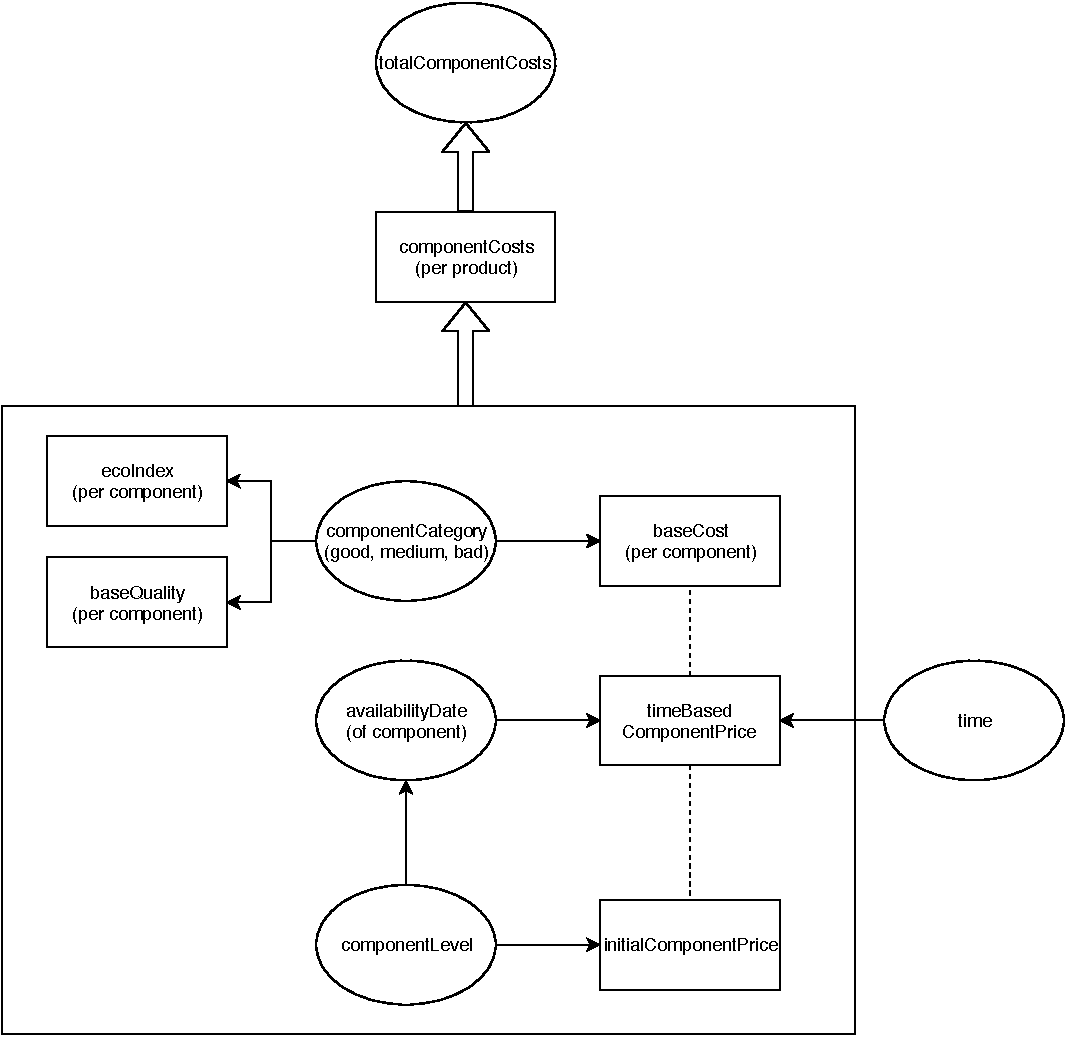
\includegraphics[width=11.5cm]{images/totalComponentCosts.pdf}
	\caption{Calculation of \textit{totalComponentCosts}}
	\label{img:totalComponentCosts}
\end{figure}

Starting from the bottom of figure \ref{img:totalComponentCosts}, the \textit{initialComponentPrice} is available for each component and depends on the \textit{componentLevel}.
The \textit{timeBasedComponentPrice} depends on the \textit{time}, on the \textit{availabilityDate} of a component, and on the \textit{initialComponentPrice}, which in turn depends on the \textit{componentLevel}.
The \textit{timeBasedComponentPrice} is dependent on the \textit{time} because we assume that a supplier produces a component in a certain level for a certain amount of time. In the first year, this is then state-of-the-art technology. However, as state-of-the-art technology rapidly become outdated and additionally new \textit{componentLevels} are released, the \textit{timeBasedComponentPrice} decreases starting from the second year on.

The \textit{timeBasedComponentPrice} is calculated by multiplying the \textit{initialComponentPrice} with the \textit{timeBasedPriceMultiplicator} (tBPM), as shown in equation \ref{Function timeBasedComponentPrice}. The \textit{timeBasedPriceMultiplicator} in turn is calculated according to the polynomic function \ref{Function timeBasedPriceMultiplicator} of fifth degree, which was interpolated from component values loosely based on historical component prices found on multiple Internet sources such as \href{https://camelcamelcamel.com}{camelcamelcamel.com}.
\begin{equation}
\label{Function timeBasedPriceMultiplicator}
\begin{aligned}
   tBPM_{c}(t_y, c) = & - 0.0001(t_y-availabilityDate_{c}+1)^5 \\
   & - 0.0112(t_y-availabilityDate_{c}+1)^4 \\
   & - 0.4239(t_y-availabilityDate_{c}+1)^3 \\
   & + 7.3219(t_y-availabilityDate_{c}+1)^2 \\
   & - 49.698(t_y-availabilityDate_{c}+1) \\
   & + 142.7889 &&
\end{aligned}   
\end{equation}
\begin{equation}
\label{Function timeBasedComponentPrice}
    tBCP_{c} (iCP, tBPM) = iCP \cdot \dfrac{tBPM}{100}
\end{equation}

\begin{figure} [H]
    \centering
	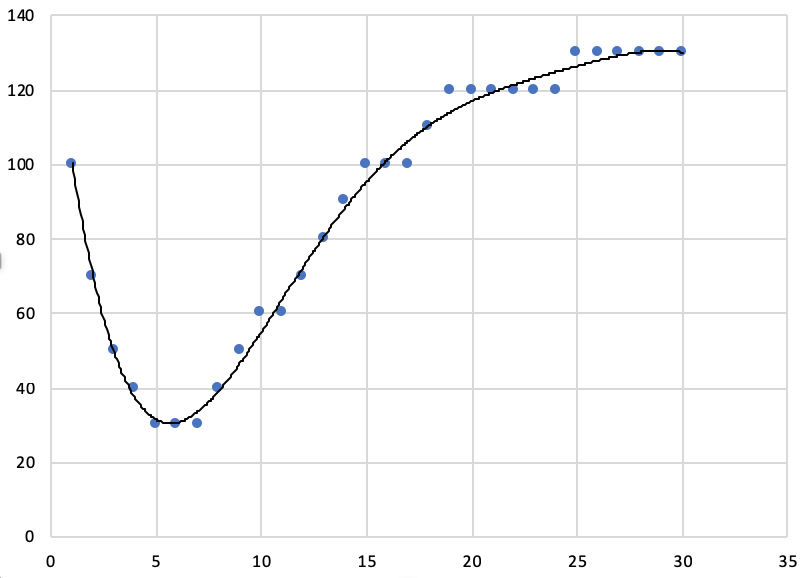
\includegraphics[width=9.5cm]{images/timeBasedComponentFunction.png}
	\caption{Function of \textit{timeBasedComponentPrice}}
	\label{img:timeBasedComponentPriceFunction}
\end{figure}
As it can be seen in picture \ref{img:timeBasedComponentPriceFunction} the \textit{timeBasedComponentPrice} decreases until the 5th year, stays stable for a short while on this reduced level, and then starts increasing again. The increase is due to the assumption that a supplier will discontinue the production of a component with a certain \textit{componentLevel} after some time because a newer level is released or available on the market. Since the supplier’s stock could be empty at this point, the component becomes a rarity. Therefore the component becomes more expensive compared to its \textit{initialComponentPrice}.\\
Afterwards, based on the \textit{timeBasedComponentPrice} and the \textit{supplierCategory} (which can either be premium, regular or cheap) a component's \textit{baseCost} is calculated. Moreover, also a component's \textit{supplierEcoIndex} and \textit{supplierQuality} depend on the \textit{supplierCategory}.\\
The \textit{componentCosts} per product can then be calculated by adding up the \textit{baseCost} of the selected components per product. All \textit{componentCosts} together then determine the \textit{totalComponentCosts} of all produced products.\\

In the following, further ideas for the procurement simulation are explained which have not yet been implemented or tested in our prototype, but which are also part of our concept.

A volume discount would allow the player to get a 10 percent discount, for example, if he buys more than 300 units of a component. We postponed this idea because our prototype does not include units in the procurement simulation yet. Currently, the player only needs to select a component and it is assumed that the desired quantity is delivered for just-in-time production. 
The aim, however, is to leave the purchase decision to the user, who would have to calculate the trade-off between the benefits of lower prices per component due to volume discounts and higher storage costs for storing all non-producible components.

% Production Simulation
\section{Production Simulation}
\label{sec:productionSim}
 \begin{quotation}
"Production is a process of combining various material inputs and immaterial inputs (plans, know-how) in order to make an output for consumption. It is the act of creating an output, a good or service which has value and contributes to the utility of individuals."\cite{noauthor_production_2019}
 \end{quotation}
The definition above provides us with the basis of the production process. In it we can already start to differentiate separate sectors, such as the Procurement Department for getting the material inputs and the HR department for providing the know-how, the human factor in production. \\
In this simulation we are going to focus on three very important indicators, namely product quality, product cost, production performance. In order to derive these indicators we will need to analyze the factors that influence them and give them proper values. 

Firstly, product quality is considered a very important element in the production simulation, nevertheless it is a very volatile concept and thus challenging to define and implement in this simulation. Often defined as conformance to requirements \cite{crosby_quality_1979}, quality is an elusive factor of production, which we have tried to frame in order to serve the scope of this project.

 Several factors that affect product quality in our CapitalismX simulation are listed below:
\begin{itemize}
\item Production Technology (PT)
\item Production Employee Skills (PES)
\item Procurement Quality (ProcQ)
\item Logistic Quality (LQ)
\item R\&D
\end{itemize}
Product quality is influenced by many elements, that in principle belong to the extend of other departments in the company. To illustrate, employee skills are included in the HR simulation, the supplier index is included in the procurement simulation, logistics and warehousing in their respective simulations, etc. \\
These elements all correlate in order to give an estimation of product quality.
All the elements have a $5$ point Likert-Scale, except from the supplier indexes.
These indexes, namely Eco-Index of the supplier $(EI_{s})$ and the Base Quality of the supplier $(BQ_{s})$ have a scale of measurement of $3$ points. They vary from good, medium to bad. In order to handle this divergence in scale, we have adjusted the supplier indexes by multiplying their sum with $\frac{5}{6}$. These indexes will be attributed to the total Procurement Quality.
\begin{equation}
ProcQ=(EIs + BQs)\times \frac{5}{6}
\end{equation}

In order to converge all the above mentioned elements and to measure Product Quality, we have compiled the following equation.
\begin{equation}
ProductQuality = (PES+PT+R\&D+LQ +ProcQ) \times 0.04_{N\footnotemark}
\label{eq:PQ}
\end{equation}
\footnotetext{N: index is normalized in the range of $[0-1]$}
 
After giving you an understanding of our concept of product quality, in the following sections we will explain the elements that  are included in this formula, and also further concepts that apply to the production process.

\subsection{Production Technology Level}
We will focus on Production Technology in this chapter, as you will encounter all the other elements in the following simulations. \\
Table \ref{table:my-label}, explains the $5$ points Likert-Scale for measuring Production Technology. This scale has a range of $[1-5]$, where $1$ is the lowest value and $5$ the highest.

\begin{table}[ht]
\centering
\begin{tabular}{|c|l|}
\hline
 Range & Production Technology\\
\hline
 1 & Depreciated  \\
 2 & Old \\
 3 & Good conditions \\
 4 & Purchased more than 5 years ago  \\
 5 & Brand New\\
\hline
\end{tabular}
\caption{Production Technology}
\label{table:my-label}
\end{table}

The technology of the machinery used in production starts at level $5$, when all machinery is new. This level can change during the game, by either increasing or decreasing. The Production Technology level can decrease one level$(-1)$ over a $5$ years time-span, due to the effects of machine depreciation. This index can decrease two levels$(-2)$, if a natural disaster such as a fire, flood or a hurricane occurs.\\
There are also possibilities to improve the production technology level after a certain period of time has passed. These actions are created to  positively influence the technology level of machinery.
\begin{itemize}
    \item Purchasing new machinery (level $5$) \\
		Purchasing new machinery immediately sets the machine's technology level to $5$, the maximum level, because the machinery is new and it complies with the measures of eco-laws and safety regulations.
\item Maintaining \& repairing $(+1)$ \\
Maintaining a machine is a regular process in all production companies. In CapitalismX, maintenance is optional for each machine, and the player can select which machine to maintain for a certain price. The price for maintenance is fixed for every machine and it improves the Production Technlolgy scale by one level. 
Repairs are also very frequent processes in production companies. Machines do not always function properly, and after using them at full capacity for a period of time they need intervening actions in order to restore them into their optimal state. In this simulation, repairs also increase the production technology scale by one level, as repairing is necessary, but it does not offer additional features to the machine.
\item Upgrading ($+2$) \\
Upgrading a machine is a process that implements new, better features into the current machine. Alongside with increasing the production technology scale by two levels, upgrading also allows increasing the individual machine production capacity by $20\%$.
\end{itemize}
When buying a new machine the prices will be set by the game mechanics. This price calculation will be decided on the capacity of each machine, since they will all have a production technology level equal to $5$. It is calculated as the sum of the base price equal to $1000cc$ with the machine capacity times $120\%$.  The supplementary $20\%$ of the price is added to the amount, as an additional payment for the retailer.
\begin{equation}
buyMachinePrice=(basePrice+MC)\times 120\%
\label{eq:buyMachine}
\end{equation}
In this simulation it is also possible to sell your current machines. A player should choose this option if he is low on CapCoins, or has purchased too many machines and they are deteriorating. The selling price will be set by the game mechanics, accordingly with equation \ref{eq:sellMachine}.
\begin{equation}
sellMachinePrice=(PT \times levelPrice_{PerPTLevel})+MC
\label{eq:sellMachine}
\end{equation}
\begin{center}
	where\\
	PT = Production Technology level \\
	MC = Machine Capacity
\end{center}
In this formula, the selling price is calculated by multiplying the current production technology with a bench-marked value of $200cc$ per production technology level and adding the machine capacity value. It is formulated as such because when the player purchases a machine its cost varies in terms of capacity. Whilst, when selling a machine not only the capacity changes between machines but also the production technology level. And it is precisely our production technology level that accounts for the loss of value effect of the machinery, otherwise known as depreciation. 
\begin{equation}
machineryDepreciation= basePrice - (PT \times levelPrice_{PerPTLevel})
    \label{eq:machineDepreciation}
\end{equation}
This approach of calculating depreciation effects is not linear, because we have to keep in mind that our machinery can be maintained or upgraded, which means they will improve their production technology level and depreciate later than other machines, which have not undergone these procedures.
\subsection{Production Investments}
The player can decide how to improve Production Performance based on several investment options. These investments are correlated with the measurements of several performance indicators, in the production simulation. The player has to use his instinct and business intuition in order to understand which metric do these investments influence and how. It is the player's decision to insert the amount of Cap-Coins(cc), that he wants to invest. \\
The available investment possibilities are:
\begin{itemize}
\item Research and Development (R\&D)
\item System Security
\item Process Automation (PA)
\end{itemize}
These investments options are also measured in our standard $5$ points Likert-Scale. The difference in these options lies in the fact that they start at level $1$, considering that in the beginnings the company has no investments operating. The increase or decrease of these indexes is dependent on the amount of CapCoins that is invested in them.

\begin{table}[ht]
\centering
\begin{tabular}{c|c|c}
\hline
 Level & Description & CapCoins$_{(cc)}$\\
\hline \hline
 1 & No Investment & $100cc$ \\
 2 & Bad & $ 500cc$\\
 3 & Normal & $1000cc$ \\
 4 & Good & $1500cc$ \\
 5 & Very good & $2000cc$\\
\hline
\end{tabular}
\caption{Levels of Production Investments}
\label{table:prod-investments}
\end{table}
As illustrated in Table \ref{table:prod-investments}, all three of these indexes will be able to change their current level by investing the corresponding amount of money.\\
Despite these investments being made once, there will come to a point in time, when they will begin loosing their added value to the production process. This loss is represented by Figure \ref{fig:InvestmentGraph}, and its corresponding function is $f(x)=5\times\exp^{-x}$. We take in consideration the $x$ range from $0$ to $10$. This graph encompasses the phenomena of "loss of added value" that we wanted to convey.

\begin{figure}[ht]
\centering
\begin{tikzpicture}[scale=0.9]
\begin{axis}[
    axis lines = left,
    xlabel = Time (Years),
    ylabel = Investment Level (Il),
    grid style = dashed,
    legend pos=north east
]

\addplot [
    domain=0:10, 
    samples=10, 
    color=red,
]
{5*e^(-x)};
\addlegendentry{$f(x)=5 \times \exp^{-x} $}
\end{axis}
\end{tikzpicture}
\captionof{figure}{\textbf{Production Investment Graph}}	\label{fig:InvestmentGraph}
\end{figure}


In order to avoid the investments to significantly lower product quality, the player must keep in mind to invest in these elements constantly over the duration of the game. Preferably, the investments should be less than $5$ years apart, since the effect of the investment reaches $0$ after this time-span.\\
There is a special event, we have implemented regarding System Security.
If the system security indicator falls below the $3^{rd}$ level threshold, incidents in the workplace and stealing inside the company will start to occur and they will negatively influence Company Image. \\
Process Automation is another investment option and it represents the company's investments towards more automated, futuristic processes. Its range is the same as the other investments and is set by the amount of money invested. We will expand this concept in section \ref{sub:PM}.
All the simulation explained in this section will not be visible to the player, in order to increase the level of difficulty of the game and make the player more perceptive to the effect of these elements. 


\subsection{Production Costs}
\label{prodCosts_simulation}

To determine the total product cost, several components have to be taken into account, as demonstrated in Figure \ref{fig:productionCosts}. The first is CP which is the sum of all component costs, since we need several components in order to have one end product. The overall employee salary would be included in the equation since all employees no matter in which department they work in, give an input and add value to the product. But we have decided to separate costs according to departments, that is why employee salary will be included in the HR costs. Another cost that we have included in our simulation is the eco-cost. You can find the details regarding eco-cost calculation in section \ref{sec:compEco-idex}. Furthermore we have incorporated machinery costs, since machinery is purchased, maintained and upgraded, we have to account these expenses to machinery costs, which are part of fixed costs. Fixed costs (FC) like electricity, depreciation costs or rent are also included because they are inevitable expenses that are present in every production company. 

\begin{figure}[ht]
	\centering
		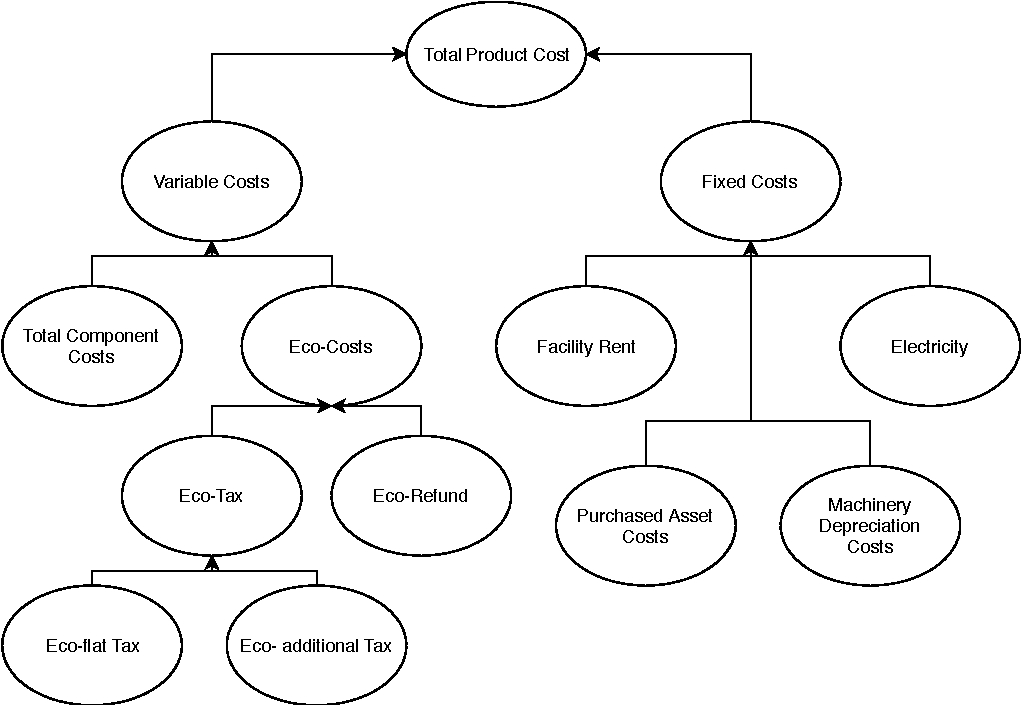
\includegraphics[scale=0.55]{images/ProductCost.pdf}
	\caption{Production Costs}
	\label{fig:productionCosts}
\end{figure}
All the above mentioned costs, add up to two major categories, variable costs and fixed costs. Together they compose the total product cost.\\
 In function \ref{eq: PC/u}, we sum up $5$ component prices, as each product can only have $5$ components per unit. In order to complete the product cost, the eco-cost and fixed costs were added and divided by the number of units in order to get a standardized dependent variable.
\begin{equation}
	Product Cost_{per Unit}= \sum_{n=1}^{n=5}CP + (\frac{Eco–Cost}{nr. Units}) + (\frac{FC}{nr. units}) 
	\label{eq: PC/u}
\end{equation}
By observing the above equation, we have described how the costs are simulated in the production process. 

%@Livja: is this place ok?
\subsection{Pricing and Selling of Goods}
\label{sec:pricing_mechanics}

Part of the production simulation is the product view. Here the player can get an overview about the costs of every single component. Also, he or she can define the market price for selling and the quantity to produce there. This view is displayed in table format for convenient reading in table \ref{table:pricingView}:

\begin{table}[ht]
\centering
\begin{tabular}{|c|c|c|c|c|c|}
\hline
 Products & \begin{tabular}{@{}c@{}}Qty to \\ Produce\end{tabular} & \begin{tabular}{@{}c@{}}Amount \\ in Stock\end{tabular} & \begin{tabular}{@{}c@{}}Total Pro- \\ duct Costs\end{tabular} & \begin{tabular}{@{}c@{}}Price for \\ Market (Sell)\end{tabular} & \begin{tabular}{@{}c@{}}Profit \\ Margin\end{tabular} \\ \hline
 Product A &  & 12 & 332,56 &  & XX.X\% \\ \hline
 Product B &  & 554 & 62,05 &   & XX.X\% \\  \hline
 Product C &  & - & 164,67 &   & XX.X\% \\ \hline
\end{tabular}
\caption{Pricing View for the Player}
\label{table:pricingView}
\end{table}

The first column, "Product" displays the name of a product, that the player when he or she chose the product portfolio. The number of rows depends on the number of products the player added to the product portfolio. 

The "Qty to Produce" field is an input field where the player can type in an integer value. The quantity a player is able to enter is depending on two different factors: the total machinery capacity and the total warehouse capacity. If the amount entered by the player is larger than the accumulated sum of overall machinery capacity, then the player sees the error message: "Your machinery capacity is not sufficient. Either produce a smaller amount or buy new machinery". This is calculated as follows in function \ref{calc:machineryCapacity1} and \ref{calc:machineryCapacity2}:
\begin{equation}
\label{calc:machineryCapacity1}
   If~entered~amount \geqslant total~machinery~capacity, 
\end{equation}
whereas 
\begin{equation}
\label{calc:machineryCapacity2}
    Total~machinery~capacity = \sum machinery~capacity
\end{equation}
Also, the amount entered must not exceed the total warehouse capacity. The total warehouse capacity is determined as seen in chapter \ref{warehouse_simulation}. To calculate the maximum amount of products that can be produced, the number of stored products needs to be subtracted from the total warehouse capacity, as shown in function \ref{maxValueToProduce}:
\begin{equation}
\label{maxValueToProduce}
    Maximum~value~of~"Qty~to~Produce" = (nWH * cWH) - nSP
\end{equation}

The next two fields are no input fields but serve the user in order to determine the quantity of products to produce and to define a market price to sell the product. First, the information field "Amount in Stock" displays the player the amount of each product in the warehouse(s), so $nSP_{per Product}$. The "Total Product Costs" show the player the total cost he or she expended for the product, which is the $ProductCost_{perUnit}$. The calculation can be found in chapter \ref{prodCosts_simulation}, function \ref{eq:PQ}.

Next, the "Price for Market (Sell)" field is an input field where the player can type in a price in CapCoins for each product. The price is restricted to a float value with two decimals and a maximum of 99,999.99. As the functions \ref{calc:priceForMarket1} and \ref{calc:priceForMarket2} show, the entered amount must not be smaller than the total product costs, otherwise the player gets the error message: "Price is smaller than the total product costs of this product. Please choose a higher price.".
\begin{equation}
\label{calc:priceForMarket1}
    Price~for~Market~(Sell) \geqslant ProductCost_{perUnit},
\end{equation}
whereas
\begin{equation}
\label{calc:priceForMarket2}
    99,999.99 \geqslant Price~for~Market~(Sell) \geqslant ProductCost_{perUnit}
\end{equation}

Last but not least, the field "Profit Margin" shows the player the profit margin for the respective product, which can be calculated as follows in function \ref{profitMargin}:
\begin{equation}
\label{profitMargin}
    Profit~Margin = \frac{Price~for~Market~(Sell) - Total~Component ~Costs}{Price~for~Market~(Sell)} * 100
\end{equation}
This value gives the player possible insights about his or her pricing strategy, as a high profit margin should only be used when using the components with the best quality and eco-index and when also the own company's eco-index and customer satisfaction is very high.

As further clarified in chapter \ref{warehouse_simulation}, the products produced per day are first collected in the warehouse and sent out to the market in the next day. For the player, no further intervention is needed. Once determined how many products to produce, the selling process starts automatically.

\subsection{Performance metrics}
\label{sub:PM}
In this section we are going to present some important metrics that help us understand how, not only quality but also production performance is measured in our game. In order to measure production performance there are several other metrics that need to be defined. \\
Equation \ref{eq: PES} shows the calculation of production employee skills. This calculation is a weighted average of the level of Process Automation and Employee Skills, which are defined in chapter \ref{sec:HRsim}. As you can notice more weight has been given to Employee Skills as it is a more relevant factor in determining our dependent variable. Process Automation on the other hand is a bit more complex as it needs to have some prerequisites fulfilled regarding employee skills. In order to increase PA according to the money invested, the player must have trained the employees in the production area, which means that the new technologies that will be implemented in production, will meet with employees that are trained to handle them. The possible trainings can be seen in section \ref{sub:KPI}. It is required to have at least $1$ production engineer trained, for each level of PA. For instance, in order to invest and have PA set in level $4$, at least $4$ production employees need to be trained in the production area.
\begin{equation}
Production Employee Skills= 0.4\times PA + 0.6\times ES
\label{eq: PES}
\end{equation}

Manufacture efficiency is measured by dividing the number of goods produced, on a daily basis, by the current number of machines times their average capacity to produce. This measure is important as it shows the player the rate in which the machinery is being utilized. This index has a range of $[0-1]$,which means if ME is close to $1$ the usage of the machinery is optimal, but if this index is low, the player should realize he should either produce more or sell some of the machinery in order to keep efficiency high and not waste resources.
\begin{equation}
ME= \frac{nr. units Produced(daily)}{nr. Machines\times avg. Capacity}  
\label{eq: ME}
\end{equation}

Production Process Productivity (PPP) is an indicator of the efficiency of our production  process. It is based on Production Technology and Production Employee Skills as indicators of the quality of the process and Manufacture Efficiency as an indicator of the efficiency of the manufacturing process.
\begin{equation}
PPP= [(PT + PES) \times ME]/10_{N\footnotemark}
\label{eq:PPP}
\end{equation}
\footnotetext{N: index is normalized in the range of $[0-1]$}
 
To conclude, in our production simulation we explained several elements that influence the production process. These elements include machinery, possible investments and performance metrics. All of these elements derive to the two most important indicators, which are product quality and production process productivity. By creating these indicators we have scratched the surface of manufacturing as a process, but they provide a strong basis in order to provide a successful Production Simulation. 

%Warehousing
\section{Warehouse Simulation}
\begin{itemize}
    \item All produced products go directly into the warehouse but it only costs if they are not sold / delivered at the same day they are produced.
    \item For each product in the warehouse at the end of the day (after all packages are delivered according the demand) the company has to pay
    \item If the warehouse is full, it shouldn't’t be possible to produce more products. That means production is limited to the storage capacity! 
    \item Storage capacity is shared between components and products. To make it a bit more realistic: components need 1/2 unit and products 1 unit
    \item number of products in the warehouse forms the basis for the number of products that can be sold
    \item Characteristics 
    \begin{itemize}
        \item can be build / bought or rented
        \item linear depreciation over 25 years, building losses every year AC/25 on value 
        \item capacity of 5000 units
    \end{itemize}
    \item Cost 
    \begin{itemize}
        \item building-costs (one time) | rental cost (monthly)
        \item maintenance costs (yearly or monthly) 
        \item Daily costs for storage = number units * storing cost per unit per day
    \end{itemize}
\end{itemize}

\section{Logistic and Support Simulation}
%Logistic
\subsection{Logistic} \label{logistic_simulation}

%\gls{eIT}  % ecoIndexTruck
%\gls{nT}   % numberTrucks
%\gls{qIT}  % qaulityIndexTruck
%\gls{cF}   % capacityInternalLogisticsFleet
%\gls{iLI}  % internalLogisticIndex 
%\gls{fCD}  % fixedCostsDelivery 
%\gls{vDC}  % variableCostsDelivered 
%\gls{cED}  % costExternalDelivery 
%\gls{dC}   % deliveryCost
%\gls{dP}   % deliveredProducts
%\gls{eIP}  % ecoIndexPartner
%\gls{qLP}  % qualityIndexLogisticPartner
%\gls{tCCLP}% totalContractualCostLogisticPartner
%\gls{vCDE} % variableCostDeliveryExternal
%\gls{rLP}  % reliabilityLogisticPartner
%\gls{sF}   % shippingFee
%\gls{eF}   % ecoIndexFleet
%\gls{qF}   % qualityIndexFleet
%\gls{eLI}  % externalLogisticIndex
%\gls{li}   % logisticIndex


%Janine
The delivery of the products always takes place at the end of the day directly from the warehouse. Basically there are three ways to manage the logistic of the company: 
\begin{itemize}
    \item The company has its own logistics fleet
    \item The company has outsourced the logistics to an external partner
    \item The company simply sends products by mail
\end{itemize}

The player can combine these variants in the way he considers best for his company. Basically, there are four logical approaches:
\begin{enumerate}
    \item The player decides to send all his products by post 
    \item The player decides to completely outsource the logistics and signs a contract with an external logistics partner
    \item The player exclusively employs his own logistics fleet and ships products that exceed his delivery capacity at high cost by post
    \item The player has his own fleet and delivers products which exceed his capacity by an external logistics partner
\end{enumerate}
	
In the following sections, the functionality of the individual variants and the costs incurred are explained in detail.


\subsubsection{Internal logistic fleet}
The internal logistics fleet consists of purchased trucks and the company's logistics employees. The quality of the company's own logistics is calculated on the basis of their characteristics and motivation.

Every truck has certain characteristics, these consist of:
\begin{itemize}
    \item A capacity of products that can be transported, this is the same for all trucks and amounts to 1000 packages. For reasons of simplification, we do not distinguish the size of individual products.  Each product is equivalent to one package. 
    \item An environmental index (\gls{eIT}) that expresses how environmentally friendly the vehicle is.
    \item A quality index (\gls{qIT})that expresses the quality of the transport.
    \item A purchase price that depends on the quality and environmental friendliness of the truck. The standard price for a truck is 100000 CapCoins. (REFERENCE https://www.motor-talk.de/forum/wie-teuer-ist-ein-neuer-lkw-t1631664.html)
    \item Monthly maintenance costs corresponding to 0,1\% of the initial purchase price divided by 12 months (REFERENCE)
    \item And a depreciation rate that is linear and amounts to 9 years for each truck (REFERENCE https://www.lexoffice.de/service/abschreibungstabelle/lkw/) 
\end{itemize}

As already described, quality and environmental friendliness influence the initial purchase price of a truck, which is 10.000 CapCoins. In order to give the player more freedom for decisions, there are basically six different truck models available for purchase, table \ref{Truck_characteristics} shows how they are composed in detail. 

The quality and the environmental index, are set randomly in the given ranges.The purchase price for the respective truck and the fixed delivery costs are calculated by multiplying the base price with the factors. These factors are also randomly assigned in a certain value range. Cause of the fact that the intervals of the individual models overlap, it can happen that a more favourable model has better properties than a more expensive one.


\begin{table}[ht]
    \centering
    \begin{tabular}{|l|r|r|r|}
    \hline
    Quality Index & Eco Index & Influence on base price & influence on fix delivery cost \\
    60 - 100      & 60 - 100   & 1.1 - 1.3   & 0.6 - 0.8       \\
    60 - 100      & 0 - 40     & 0.9 - 1.1   & 0.8 - 1.1       \\
    30 - 70       & 60 - 100   & 1.0 - 1.2   & 0.7 - 0.9       \\
    30 - 70       & 30 - 70    & 0.8 - 1.1   & 0.9 - 1.1       \\
    0 - 40        & 30 - 70    & 0.7 - 0.9   & 1.0 - 1.2       \\
    0 - 40        & 0 - 40     & 0.6 - 0.8   & 1.1 - 1.3       \\
    \hline
    \end{tabular}
    \caption{Truck characteristics and calculations}
    \label{Truck_characteristics}
\end{table}

The total capacity thus results from the number of trucks (\gls{nT}) in the company's own logistics fleet. 
\begin{equation}
    Capacity internal logistics fleet (\gls{cF}) = 1000 * nT
\end{equation}

The overall quality internal logistics, the so-called Internal Logistic Index (\gls{iLI}), is calculated on the basis of the quality and environmental friendliness of the individual trucks.  
\begin{equation}
\begin{aligned}
    Eco Index Fleet (\gls{eF}) = Sum (eIT) / NT \\
    Quality Index Fleet (\gls{qF}) = Sum (qIT) / NT \\
    Internal Logistic Index (\gls{iLI}) = eF * 0,2 + qF * 0,8 \\
\end{aligned}
\end{equation}

Of course, the delivery of the products entails costs for the company. These consist of the fixed costs for the ride of a truck (\gls{fCD}) and the variable costs per delivered package (\gls{vCD}). 
A delivery by truck in principle costs 2000 CapCoins. Like the purchase price, the fixed delivery costs also vary on the basis of quality and eco index. The variable delivery costs per product are the same for each truck and amount to 2 CapCoins.

The cost of a delivery thus depends on the total number of products to be delivered (\gls{dP}). 
The case that the number of products to be delivered exceeds the total capacity of the internal delivery fleet must be considered separately. The additional costs incurred by an external delivery (\gls{cED}) can either be caused by a contractual external logistics partner or by sending the packages by post. How these costs are composed in detail is described in the following sections. 
\begin{equation}
\begin{aligned}
Delivery cost (\gls{dC}) = if ( dP = cF ) { (( dP / 1000) * fCD) + ( dP * vCD) } \\
elseif ( dP < cF ) { (round up to next int ( dP / 1000) * fCD ) + ( dP * vCD) } \\
else { ( nT * fCD ) + ( nT *1000 * vCD ) + cED }
\end{aligned}
\end{equation}

\subsubsection{External logistic Partner}
In addition to his own logistics fleet, the player has the option of forming a contract with an external logistics partner. It is possible to outsource the complete product delivery to this partner or only products that exceed the delivery capacity of the own fleet. Basically, only one partner can be contracted at a time, but he can be fired at any time and replaced by another partner available on the market. 
The external logistics partners also have certain characteristics that influence the quality of the delivery: 

\begin{itemize}
    \item An eco index (\gls{eIP}) that expresses how environmentally friendly the external partner is working (0-100)
    \item A Quality Index (\gls{qLP}), which expresses how good the quality of the partner's delivery is (0 -100)
    \item A reliability index (\gls{rLP}), which expresses how reliable the partner is
    \item Contractually agreed monthly fixed costs (\gls{tCCLP}) for the provision of the service, which are based on the quality, environmental friendliness and reliability of the external logistics partner. The basic price is 1000 CapCoins 
    \item And contractually agreed variable delivery costs (\gls{vCDE}) per delivered product.These are generally 5 CapCoins, but this price also depends on the characteristics of the service provider
\end{itemize}

The table \ref{External_logistic_partner_characteristics} shows how exactly the costs are related to the properties and which characteristics can occur in the game. Within the specified value ranges, the values are assigned randomly. 
The contractual costs and the variable costs are calculated by the initial price multiplied by the factor that depends on the partner characteristics.

\begin{table}[ht]
    \centering
    \begin{tabular}{|l|r|r|r|r|}
    \hline
    Quality Index & Eco Index & Reliability Index & influence tCCLP & influence vCDE \\
    60 - 100      & 60 - 100   & 60 - 100  & 1.1 - 1.3    & 0.7 - 0.9     \\
    60 - 100      & 30 - 70    & 30 - 70   & 1.0 - 1.2    & 0.8 - 1.0     \\
    60 - 100      & 0 - 40     & 60 - 100  & 1.0 - 1.2    & 0.8 - 1.0     \\
    30 - 70       & 60 - 100   & 0 - 40    & 0.9 - 1.1    & 0.9 - 1.1     \\
    30 - 70       & 30 - 70    & 30 - 70   & 0.9 - 1.1    & 0.9 - 1.1     \\
    30 - 70       & 0 - 40     & 60 - 100  & 0.9 - 1.1    & 0.9 - 1.1     \\
    0 - 40        & 60 - 100   & 30 - 70   & 0.9 - 1.1    & 0.9 - 1.1     \\
    0 - 40        & 30 - 70    & 30 - 70   & 0.8 - 1.0    & 1.0 - 1.2     \\
    0 - 40        & 0 - 40     & 0 - 40    & 0.7 - 0.9    & 1.1 - 1.3     \\
    \hline
    \end{tabular}
    \caption{external Logistic Partner characteristics and cost calculations}
    \label{External_logistic_partner_characteristics}
\end{table}

The total influence of an external partner company is measured by the External Logistics Index (\gls{eLI}). Depending on how high its reliability is, different priorities are set in the calculation. The following formula shows the exact calculation: 
\begin{equation}
\begin{aligned}
    if (rLP ≤ 40) eLI = { (rLP*0,5 + 0,5*(qLP*0,8 + eIP*0,2)) } \\
    else eLI = { (rLP*0,4 + 0,6*(qLP*0,8 + eIP*0,2)) }
\end{aligned}
\end{equation}

If the player decides to delivered all products by an external logistics partner, the daily costs for the company are calculated as follows:
\begin{equation}
    Cost external delivery (cED) = dP * vCDE
\end{equation}

If the company has its own logistics fleet, the products are initially delivered via it. However, if the company's own capacities are not sufficient, the remaining products are taken over by the external partner. In this case, the costs are calculated as follows: 
\begin{equation}
    cED = ( dP – cF ) * vCDE
\end{equation}

If the company has not engaged an external partner and exceeds the delivery capacity, the remaining products will be sent by post. For each package there will be a shipping fee (\gls{sF}) of 15 CapCoins. Also in this case delivery quality and environmental friendliness are included. The quality index is basically 60 and the eco index 40. The external delivery costs are calculated as follows:  
\begin{equation}
    cED = ( dP – cF ) * sF
\end{equation}

The overall quality of the company's logistics as perceived by its customers is expressed by the logistics index. This includes both the internal logistics and the external logistics in proportion to the products delivered. The following formula shows the exact calculation of the Logistic Index (\gls{lI}):
\begin{equation}
\begin{aligned}
    if ( dP > cF ) lI = { ((( dP – cF) * eLI ) + ( cF * iLI )) / dP} \\
    elseif ( dP = cF ) lI = { cF * iLI } \\
    else lI = { dP * iLI }  
\end{aligned}
\end{equation}
%Support
\subsection{Product Support}  \label{product_support_simulation}

%Janine
In addition to the product itself, a product support strategy is also necessary. This strategy should not only consist of maintaining the actual product functionality, but should also include further services for the customer in order to provide him with the greatest possible value with his product \cite{markeset_design_2003}. Additional services could for example be a mobile app or and actively managed community.  
In Capitalism X, the player is offered various options how he wishes to design the product support for his products. Table \ref{Support_types} shows the different services that can be purchased from an external partner, how they influence the \textit{totalSupportTypeQuality} (\gls{tSTQ}) with there \textit{typeQuality} (\gls{sTQ}) and the monthly \textit{typeCost} (\gls{cST}). The variants can be combined by the player as desired. If no option is selected, this automatically means that no support is offered.
Before the company can offer product support to its customers, the player must hire an external support partner. Basically only one partner can be hired at a time, but he can be fired at any time.

\begin{table}[ht]
    \centering
    \begin{tabular}{|l|r|r|}
    \hline
    Support type & sTQ & cST \\
    \hline
    No product support   & -10   & 0    \\
    Online self service  & 0     & 50   \\
    Online support       & 20    & 100  \\
    Telephone support    & 30    & 250  \\
    Store support        & 40    & 400  \\
    Additional services  & 10    & 50   \\     
    \hline
    \end{tabular}
    \caption{Support type influence and costs}
    \label{Support_types}
\end{table}

The \textit{totalSupportTypeQuality} is calculated from the various support types offered; this is simply the sum of the support types. The quality of the \textit{totalSupportQuality} (\gls{tSQ}) of the company is influenced not only by the offered support types but also by the dedicated support company, more precisely its \textit{qualityIndex} (\gls{qSP}). The calculation is done as follows:
\begin{equation}
\label{func:totalProductSupport}
\begin{aligned}
    tSQ = &
    \begin{cases}
        0.4 \cdot qSP + 0.6 \cdot tSTQ & \text{if } qSP \leq  50\\
        0.3 \cdot qSP + 0.7 \cdot tSTQ & \text{otherwise}
    \end{cases}
\end{aligned}
\end{equation}

The \textit{totalSupportCost} (\gls{tSC}) are calculated from the sum of the monthly \textit{typeCost} and the \textit{contractualCost} (\gls{cSP}) for cooperation with the partner company.
\begin{equation}
\label{func:totalSupportCost}
    tSC = \sum cST + cSP
\end{equation}

\section{Marketing Simulation}
\label{markting_simulation}
%Company Image
\subsection{Company Image} \label{company_image}
%Philipp and Janine

The company image is a very important KPI to measure the company reputation. The company image is the sum of many small activities which leaves a footprint that can be recognized with the company. Single activities can improve or destroy the \textit{companyImage} (\gls{cI}) from the point of view of individuals. The goal of a high valued company image is of course monetary benefit. Therefore, activities which tend to increase the \textit{companyImage} are not for free and it is always a difficult assessment whether to invest in a certain activity or not. In the game we concentrated on factors which can be realistically and interestingly be influenced by the player.

\begin{table}[h]
\centering
\begin{tabular}{|l|r|r|r|}
\hline
\multicolumn{1}{|l|}{\textbf{Action}} & \multicolumn{1}{l}{\textbf{Costs in CapCoins}} & \multicolumn{1}{l}{} & \multicolumn{1}{l|}{} \\ \hline
CSR (in \% of profit)     & depending on profit &                   & \\
Support Refugee Projects  & 1000        &                   & \\
  & \underline{newspaper} & \underline{TV}      &  \underline{Online} \\
Marketing Campaigns       & 5000                & 10000             & 100000 \\
\hline
\end{tabular}
\caption{Cost campaigns}
\label{cost_campaigns}
\end{table}

\begin{table}[]
\begin{tabular}{|l|r|r|r|}
\hline
\multicolumn{1}{|l|}{\textbf{Action}}             & \multicolumn{1}{l|}{\textbf{Points}} & \multicolumn{1}{l|}{}       & \multicolumn{1}{l|}{}   \\ \hline
\textbf{Social engagement}        &       &       &  \\
\underline{CSR (in \% of profit)} & 0     &       &  \\
\textless 1\%                     & 1     &       &  \\
1\% \textless 2\%                 & 2     &       &  \\
2\% \textless 5\%                 & 3     &       &  \\
5\% \textless{}                   & 4     &       &  \\
\underline{Support refugee projects}  &   &       &  \\
never                             & 0     &       &  \\
1 project per year                & 1     &       &  \\
at least 2 projects per year      & 2     &       &  \\
&  &  &  \\ \hline
\textbf{Marketing Campaigns}  & \textbf{Newspaper} & \textbf{Television} & \textbf{Online} \\ \hline
\underline{Promote environmental friendly supplier}   & & & \\
never                             & 0    & 0      & 0 \\
1 time per year                   & 1    & 1.5    & 2 \\
at least 2 times per year         & 1.5  & 2      & 2.5 \\
\underline{Promote environmental friendly production} & & & \\
never                             & 0    & 0      & 0 \\
1 time per year                   & 1    & 1.5    & 2 \\
at least 2 times per year         & 1.5  & 2      & 2.5 \\
\underline{Green marketing campaign} & & & \\
never                             & 0    & 0      & 0 \\
1 time per year                   & 1    & 1.5    & 2 \\
2 times per year                  & 2    & 3      & 4 \\
3 times per year                  & 3    & 4.5    & 6 \\
at least 4 times per year         & 3.5  & 5      & 6.5  \\
\underline{Diversity Campaign}    & & & \\
never                             & 0    & 0      & 0 \\
1 time per year                   & 0.5  & 1      & 1.5  \\
at least 2 times per year         & 1    & 1.5    & 2 \\
\underline{Promote Products} & & & \\
never                             & 0    & 0      & 0 \\
1 time per year                   & 1.5  & 2      & 2.5  \\
2 times per year                  & 3    & 4      & 5.5  \\
3 times per year                  & 4.5  & 6      & 8 \\
at least 4 times per year         & 5    & 6.5    & 8.5  \\
\hline
\end{tabular}
\caption{Actions influencing the Company Image}
\label{calculation_CI}
\end{table}

The total sum of the above possible choices is the total \textit{companyImage}. The score can reach values from 0 to 28 as it is the case for the \textit{totalJobSatisfaction}. In order to build also here a more realistic representation we figured out that the marginal benefit of an increase of the \textit{companyImage} increases with the collected amount of points. Therefore, we manipulated also this formula and came up with the function that can be seen in figure \ref{fig:scaling}.

\begin{figure}[h]
    \centering
    \begin{tikzpicture}
    \begin{axis}[
        axis lines = left,
        xlabel = Original Scale (\gls{oS}),
        ylabel = Company Image  (cIS),
        grid style = dashed,
        legend pos=north west
    ]
    \addplot [
        domain=0:28, 
        samples=28, 
        color=red,
    ]
    {x^2/7.84};
    \addlegendentry{$cIS=\frac{oS^2}{7.84}$}
    \end{axis}
    \end{tikzpicture}
    \caption{Scaling function companyImage}
    \label{fig:scaling}
\end{figure}

The original scale of 0 to 28 is squared and divided by the factor of 7.84 in order to map the original scale on a scale of 0 to 100. In this case the rational behind the mapping is the fact that little activities do not have such  a big influence on the overall \textit{companyImage}. When a company starts to combine all its activities it can generate huge impact and publicity which leads to a strong increase of the \textit{companyImage}.


\subsubsection{Press Releases} \label{press_releases}

In addition to marketing campaigns and social engagement projects, the player can also publish press releases. Each press release has a name and an impact, but it is only effective if an unexpected event occurs beforehand. Chapter \ref{sec:ectEvent} describes the concept of external events in detail. At this point, only those events are mentioned whose effects can be mitigated by timely and appropriate press releases.
In order for the press release to have a mitigating effect, they must be published by the player at the latest 10 days after the external event. If it happens later, the release will no longer affect the damage caused by the event. The player has three different press releases to choose from: 
\begin{itemize}
    \item Privacy and security efforts: The aim of this press release is to give customers the feeling that their data is in good hands and is protected and processed with the necessary care.  
    \item Guaranteed delivery times: This statement guarantees customers that they will receive their products promptly, even in difficult situations. 
    \item Apology: This press release allows the company to publicly apologize to the public for its behavior or inconvenience.
\end{itemize}

Table \ref{press_release_events} shows which press releases in combination with which external events show their impact and which influence they have.

\begin{table}[h]
\begin{tabular}{|l|l|l|l|}
\hline
\multicolumn{1}{|c|}{\textbf{Press release}}    & \multicolumn{1}{c|}{\textbf{External event}}                                & \multicolumn{1}{c|}{\textbf{Impact event}} & \multicolumn{1}{c|}{\textbf{Effect press release}} \\ \hline
\begin{tabular}[c]{@{}l@{}}Pivacy and \\ security efforts\end{tabular} & \begin{tabular}[c]{@{}l@{}}Computer \\ virus attacks\end{tabular}           & \begin{tabular}[c]{@{}l@{}}pA - 50\% \\ for 3 months\end{tabular}    &  \begin{tabular}[c]{@{}l@{}}only pA - 30\% \\ for 3 months\end{tabular}                          \\ 
\begin{tabular}[c]{@{}l@{}}Guaranteed \\ delivery times\end{tabular}   & Strikes                                                                     & -80\% pDA                                  & only -60\% pDA                                     \\ 
\begin{tabular}[c]{@{}l@{}}Guaranteed \\ delivery times\end{tabular}   & \begin{tabular}[c]{@{}l@{}}Eco activists\\ block roads\end{tabular}         & -70\% cF                                   & only -50\% cF                                      \\ 
Apology                                                               & \begin{tabular}[c]{@{}l@{}}Company brand \\ reputation plunges\end{tabular} & -20\% cI                                   & only -10\% cI                                      \\ \hline
\end{tabular}
\caption{Combination press releases and external events}
\label{press_release_events}
\end{table}

If the player publishes press releases regardless of these external events, they are simply ignored by the population, which means that they have no influence on the course of the game but cost the company money. How much a press release costs can be seen in the table \ref{cost_press_releases}. 

\begin{table}[ht]
\centering
\begin{tabular}{|l|r|r|}
\hline
\textbf{Press release}        & \textbf{price in cc}   
\\ \hline
Privacy and security efforts  &    200 \\
affordable prices             &    100 \\
guaranteed delivery times     &    100 \\
apology                       &    150 \\
\hline
\end{tabular}
\caption{Cost press releases}
\label{cost_press_releases}
\end{table}


%Employer Branding
\subsubsection{Employer Branding}\label{employer_branding}
%Philipp

\gls{eB}    % employerBranding
\gls{cI}    % companyImage
\gls{tJS}   % totalJobSatiscation

The employerBranding (eB) is the score which is reported to the external world in order to measure the value of the company as an employer in total. This score is comparable to the total score for companies which is presented on websites like kununu or glassdoor. The employer branding is a combined score out of the Job Satisfaction and the Company Image. As the Company Image implicitly incluences the Job Satisfaction rating it is weighted with 0.4 in the calculation of the employer branding score. The general formula is
\begin{center}
\texttt{eB = 0.4 * cIS + 0.6 * tJS} \\
\texttt{with} \\
\texttt{cI = companyImage}   \\
\texttt{tJS = totalJobSatisfactione}
\end{center}

In order to make the employer branding rating more realistic, we need to think about extreme cases where either the employee satisfaction or the company image is rated very low. The usage of a simple weighted average would have the effect that values of $tJS = 100$ and $cI = 0$ lead to an overall score of 60.
Therefore we need to include an indicator function which incorporates a punishment for smaller values.
This can be done by incorporating a multiplier which is based on an IF statement. See the \textit{Excel} implementation below:
\begin{center}
    $=ROUND(((0.4*cI+0.6*tJS)*IF(cI<30,0.5,IF(cI<60,0.8,IF(cI>60,1))))/10,0)$
\end{center}

The following pseudo code explains the statement above.

\begin{itemize}
    \item score = 0.4*CI + 0.6*tJS
    \item IF CI $\leq$ 30 THEN Employer Branding = Employer Branding * 0.5
    \item ELSEIF CI $\leq$ 60 THEN Employer Branding = Employer Branding * 0.8
    \item ELSEIF CI $\geq$ 60 THEN Employer Branding = Employer Branding * 1
\end{itemize}

By this we ensure a sufficient punishment of the overall Employer Branding score. To achieve this we need to create a matrix and a 3D graph to visualize the possible implications on the employer branding. Graphic \ref{img:EBS} shows the implications of the two input parameters on the Employer Branding.

\begin{figure}
	\centering
	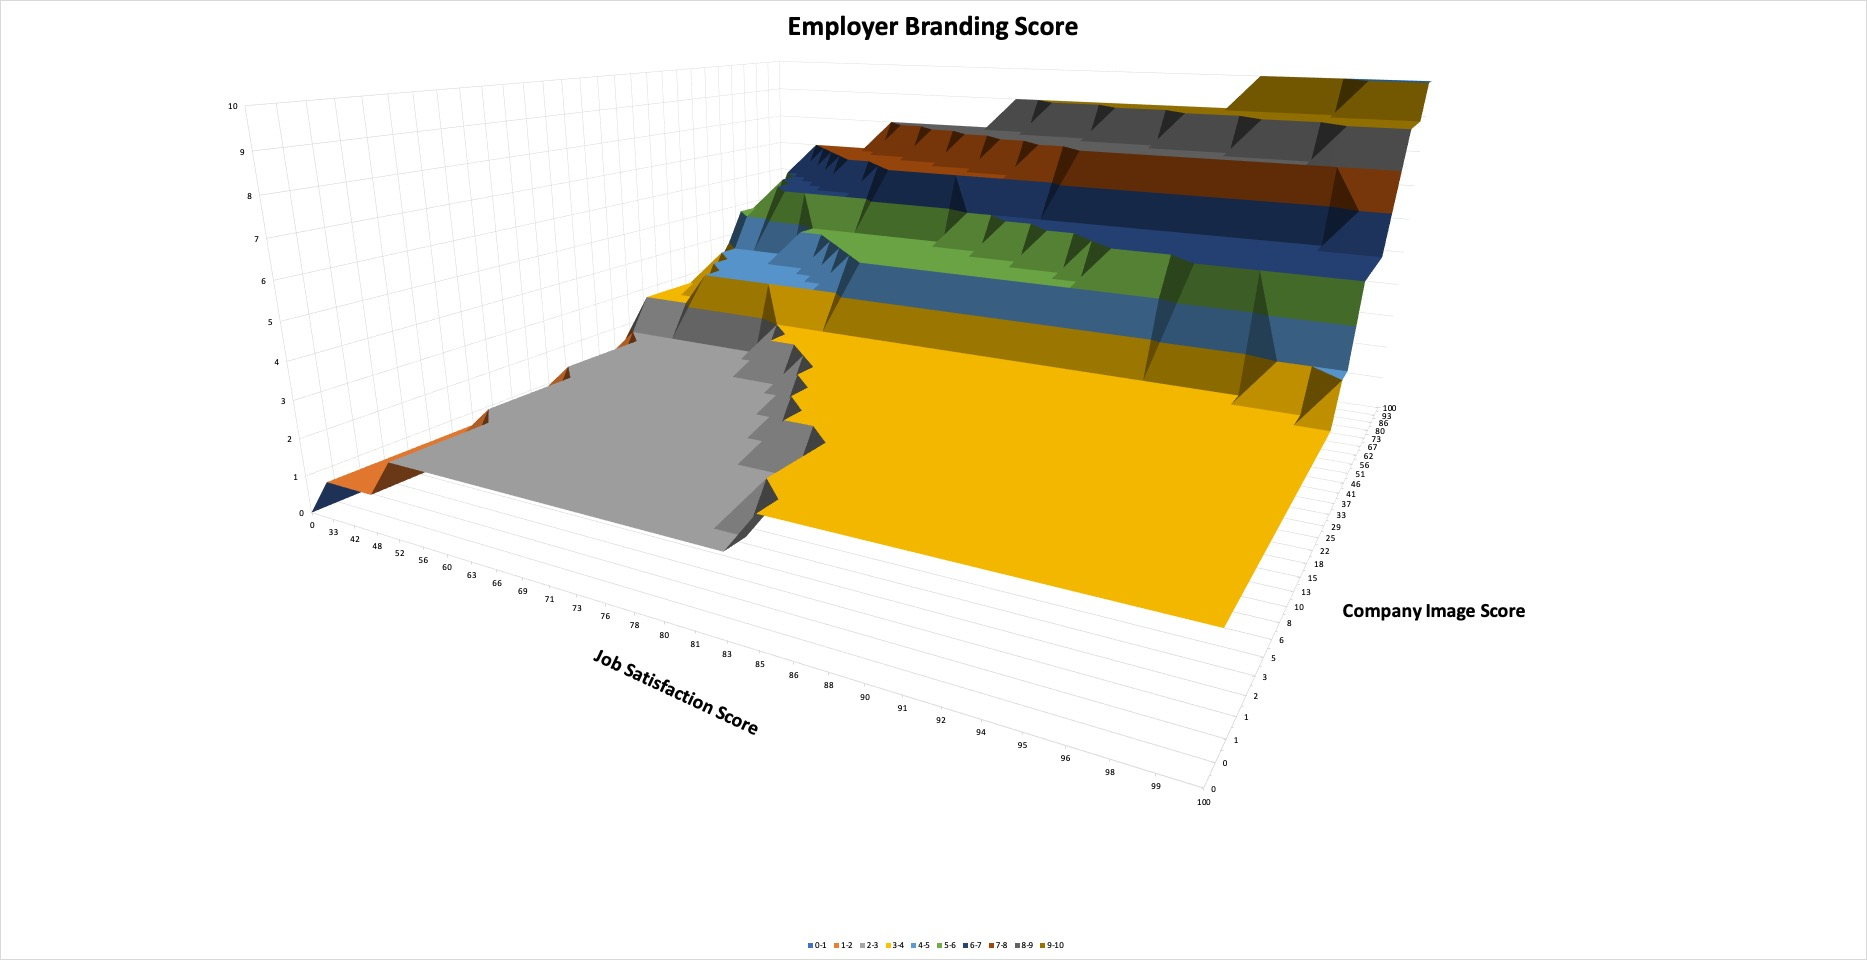
\includegraphics[width=12.5cm]{images/EBS.jpg}
	\caption{Employer Branding Score Calculation}
	\label{img:EBS}
\end{figure}
%Market Research
\subsection{Market Research} \label{market_research_simulation}

%Janine
Market research is the collection and analysis of data with the aim of better understanding the market and customers. This information can be of great advantage for the management of a company \cite[Chapter~1.2]{mooi_introduction_2018}.\\

If a company or an institution wishes to collect data directly from the customer, there are basically two different procedures. The first is to observe customer behaviour and the second is to ask customers directly. This type of data collection leads to so-called primary data \cite[Chapter~4.4]{mooi_getting_2018}.\\

As part of CapitalismX, we only consider direct customer surveys via various media. Basically there are four different \textit{dataCollectionMethods} to conduct a survey, these are personal interviews (\gls{PInt}), telephone interviews (\gls{TInt}), mail surveys (\gls{MSur}) and online surveys (\gls{OSur}). Table \ref{MR_survey_types_characteristics} shows some important features of surveys and how each survey type performs in them \cite[Chapter~4.4.2.2]{mooi_getting_2018}.\\

\begin{table}[ht]
\centering
\begin{tabular}{|l|r|r|r|r|}
\hline
                                & PInt    & TInt    & MSur   & OSur \\
\hline                              
explain a complex issue         & ++    & +     & -    & --  \\
demonstrate trial products      & ++    & -     & -    & -   \\
response rate                   & +     & o     & -    & -   \\
influence of the interviewer    & --    & -     & o    & o   \\
possibility of asking questions & ++    & +     & --   & --  \\
length of the field phase       & o     & +     & -    & -   \\
cots                            & --    & -     & +    & ++  \\
quality of the data             & ++    & +     & -    & --  \\
\hline
\end{tabular}
\caption{Characteristics personal survey types}
\label{MR_survey_types_characteristics}
\end{table}

The characteristics of the various \textit{dataCollectionMethods} naturally also affect the results of market research \cite[Chapter~4.4.2.1]{mooi_getting_2018}. For example the \textit{time} for an online survey to produce usable results is longer than for a personal interview. Overall, the \textit{quality} of the data is best through personal surveys, followed by telephone surveys, mail surveys and worst online surveys. Looking at the \textit{price} of a survey, it's the other way around, web surveys are the cheapest and personal interviews the most expensive. 

In principle, the player can decide whether the market research should be carried out by the company itself or by an external market research institute. If he decides to conduct the surveys internally, he can choose between the various methods of primary data collection and thus influence the \textit{quality} of the results himself. 

The \textit{quality} at this point expresses the extent to which the result data can deviate from the exactly calculated results. If the data collection is carried out by an institute, the data is determined by telephone interviews by default. The percentage influence on the \textit{price} of a market statistic by the choice of the \textit{dataCollectionMethods}, the \textit{time} between the commission of the survey and the results as well as the impact on the \textit{quality} of the study can be seen in Table \ref{MR_survey_types_influence}. 

\begin{table}[ht]
\centering
\begin{tabular}{|l|r|r|r|r|}
\hline
                                 & PI           & TI             & MS             & OS \\
influence on the price           & 150\%        & 125\%          & 110\%          & 100\%   \\
time lack between results        & 1 day        & 3 days         & 7 days         & 12 days   \\
influence on the data quality    & no errors    & up to +/- 1\%  & up to +/- 2\%  & up to +/- 4\%   \\
\hline
\end{tabular}
\caption{Influence personal survey types}
\label{MR_survey_types_influence}
\end{table}

The player can basically choose between three different \textit{MarketResearchs}, which are created on the basis of the previously collected data. These statistics cover price sensitivity of customers, customer satisfaction and general market data. 
The \textit{price} for the individual market statistics can be taken from the table \ref{MR_report_price}. The total cost of conducting internal market research is determined by the product of the base price of the respective statistics and the influence on the \textit{price} of the chosen \textit{dataCollectionMethods}. The costs of the external execution correspond to the final costs that the company has to pay. 
The following sections describe the market statistics available to the player in detail. \\

\begin{table}[ht]
\centering
\begin{tabular}{|l|r|r|}
\hline
                             & internal base price  & external price \\
price sensitive report       & 2.500                & 3.200     \\
customer satisfaction report & 2.000                & 2.500     \\
market statistic research    & 1.000                & 1.150     \\
\hline
\end{tabular}
\caption{prices market research reports}
\label{MR_report_price}
\end{table}

\subsubsection{Price Sensitive Research}
This report includes a price sensitivity analysis for a previously selected product in the company's product portfolio. The analysis shows how \textit{margin}, \textit{salesFigures} (\gls{sFig}), \textit{productCosts} and \textit{marketShare} change when the \textit{salesPrice} (\gls{sP}) changes. All other factors are kept constant for the calculations. The result is divided into nine price steps, from -20\% to +20\% in 5\% steps. These relate to the current sales price of the product in question. The hypothetical values are calculated as follows:
\begin{equation}
    \begin{aligned}
       for +5\% ~to~ +20\%: x = (\frac{100 \cdot new value}{ref value}) \text{-} 100\\
       % for +5\% to +20\%: x = ((100 \cdot new value) / ref value) – 100 \\
       for -5\% ~to ~-20\%: x = \frac{1-(\frac{new value}{ref value})}{100}
       % for -5\% to -20\%: x = ((1 - (new value / ref value)) / 100
    \end{aligned}
\end{equation}

Table \ref{MR_price_sensitive} shows the structure of a price sensitive report. 

\begin{table}[ht]
\centering
\begin{tabular}{|l|r|r|r|r|r|r|r|r|r|}
\hline
key figures             & -20\% & -15\% & -10\% & -5\%  & 0\%   & +5\%  & +10\% & +15\%   \\
salesPrice            &       &       &       &       &       &       &       &         \\
productCosts           &       &       &       &       &       &       &       &         \\
margin                  &       &       &       &       &       &       &       &         \\
salesFigures            &       &       &       &       &       &       &       &         \\
marketShare            &       &       &       &       &       &       &       &         \\
margin change           &       &       &       &       &       &       &       &         \\
marketShare change     &       &       &       &       &       &       &       &         \\
profit             &       &       &       &       &       &       &       &         \\
profit change             &       &       &       &       &       &       &       &         \\
\hline
\end{tabular}
\caption{Structure price sensitive report}
\label{MR_price_sensitive}
\end{table}

\subsubsection{Customer Satisfaction Research}
This report allows the player to see an overview of \textit{customerSatisfaction} over the last four quarters. The player can choose whether the result should refer to the entire company, i.e. all products, or only to a specific product. Table \ref{MR_customer_satisfaction} illustrates the structure of the customer satisfaction report. \\

\begin{table}[ht]
\centering
\begin{tabular}{|l|r|r|r|r|}
\hline
            & quarter 1   & quarter 2  & quarter 3 & quarter 4 \\
product 1   &             &            &           &           \\
product 1   &             &            &           &           \\
product 1   &             &            &           &           \\
...         &             &            &           &           \\
total       & average     & average    & average   & average   \\
\hline
\end{tabular}
\caption{Structure customer satisfaction report}
\label{MR_customer_satisfaction}
\end{table}

\subsubsection{Market Statistic Research}
This analysis provides various market information on product level. This means that the key figures for the products are provided individually and also the average for the entire company. The report contains the current \textit{salesPrice}, \textit{marketShare}, \textit{salesFigures} and \textit{totalProductQuality}. Table \ref{MR_market_statistic} is an example for the structure of the report. \\

\begin{table}[ht]
\centering
\begin{tabular}{|l|r|r|r|r|}
\hline
                    & product 1   & product 2  & product 3 & ...       \\
salesPrice          &             &            &           &           \\
marketShare         &             &            &           &           \\
salesFigur          &             &            &           &           \\
totalProductQuality &             &            &           &           \\
totalProcurementQuality  &             &            &           &           \\
componentCost       &             &            &           &           \\
margin              &             &            &           &           \\
\hline
\end{tabular}
\caption{Structure market statistic report}
\label{MR_market_statistic}
\end{table}
%Lobbyist
\subsection{Lobbyist} \label{lobbyist_simulation}
%Janine

If the company is in contact with a lobbyist, he tries to mitigate negative government decisions on the company. For its services the lobbyist demands a monthly compensation \textit{price}. The effect of the lobbyist is reflected by the \textit{taxRate}. 

Only one lobbyist can be assigned at a time, if the player wishes to hire another lobbyist, he must first fire the current one. Each lobbyist has a \textit{type}, a \textit{price} and a \textit{taxRate}. The \textit{type} determines how influential the lobbyist is, more precisely how high the \textit{taxRate} is due to his influence. The player can choose between four different lobbyists: Mayor, Worker’s Union Leader, Congressman and Senator. The Senator is the most influential but also the most expensive lobbyist. Table \ref{influence_lobbyist} shows the relationship between \textit{type}, \textit{taxRate} and \textit{price}. 

\begin{table}[ht]
\centering
\begin{tabular}{|l|r|r|}
\hline
Type                    & taxRate   & price in cc \\ \hline
Mayor                   & 18\%      & 1000     \\
Worker's Union Leader   & 16\%      & 1000     \\
Congressman             & 13\%      & 5000     \\
Senator                 & 10\%      & 10000     \\
\hline
\end{tabular}
\caption{Influence and price lobbyist}
\label{influence_lobbyist}
\end{table}

In order to find out which lobbyist is the most rewarding one for the company, the player must calculate the amount of the tax reduction and compare it with the \textit{price} incurred by the lobbyist.
 



 





%Management Consultancy
\subsection{Management Consultancy} \label{management_consultancy_simulation}
%Janine
In Capitalism X, the player has the option of engaging a business consultant to give him advice on how to make the company more successful. 
The consulting firm searches for possible points in the company which can be optimized and presents them to the player.

There are basically three different types of consulting firms: world-famous firm, local consultancy and student consultancy. These differ in their expertise and level of reputation. The more famous the organization is, the more expensive it is. Table \ref{mng_consultancy} shows the prices of the business consulting firms. 

\begin{table}[ht]
\centering
\begin{tabular}{|l|r|r|}
\hline
Consultancy type        & name  & price in cc \\ \hline
World-famous firm       & O'Reilly \& Company     & 5000     \\
Local consultancy       & Sinoido Consulting     & 3000     \\
Student consultancy     & Wannabe Consultants    & 1000     \\
\hline
\end{tabular}
\caption{Management consultancies}
\label{mng_consultancy}
\end{table}

The concept of management consulting is that they search for the relatively weakest KPI of the company. Since the different key figures do not all have the same significance for the company result, it is important to weight them for the analysis.
Table \ref{mngc_weighting} shows the key figures which are evaluated by the business consulting company and how they assess their importance.
The company with the greatest expertise meets with its assessment pretty much exactly the interrelationships implemented in CapitalismX. The other companies have slightly different views on how important the respective indicators are. 
The worst index of the company is determined by multiplying the current value by the respective weighting. The lowest of the resulting values represents the key figure with the highest optimization potential and is therefore communicated to the company. 
 
\begin{table}[!hp]
\centering
\begin{tabular}{|l|r|r|r|}
\hline
KPI                     & World-famous c.   & Local c.   & Student c.\\ \hline
totalSupportQuality     & 0.8               & 0.85       & 0.9       \\
logisticIndex           & 0.9               & 0.9        & 0.95      \\
companyImage            & 0.85              & 0.9        & 0.8       \\
productionTenology      & 0.7               & 0.65       & 0.6       \\
manufactureEfficiency   & 0.8               & 0.8        & 0.85      \\
totalJobSatisfaction    & 0.95              & 0.9        & 0.9       \\
\hline
\end{tabular}
\caption{KPI weighting management consultancies}
\label{mngc_weighting}
\end{table}



% Customer Satisfaction and Demand Calculation
% Customer Satisfaction
\section{Customer Simulation} 
\label{sec:customsim}

\subsection{Customer Satisfaction}
\label{customerSatisfaction}
In this game, the customer simulation is a weighted combination of the \textit{salesPrice}, the \textit{productQuality} and the \textit{customerSatisfaction} (\gls{cS}).
This means that the \textit{productPrice}, the \textit{productQuality} and the \textit{customerSatisfaction} are the three key indicators for customers' buying decisions. Thus, these three variables determine the extent to which customers are interested in buying a product or not.

How exactly the customer interest is calculated is discussed in detail in chapter \ref{demandCalc}. The prerequisite for this is the calculation of \textit{customerSatisfaction}, which will be discussed in more detail in this chapter.

As well as in reality, the \textit{customerSatisfaction} plays an important role in terms of the number of products sold and thus in terms of sales. \cite{deptolla_effects_2004} In CapitalismX, the \textit{salesFigures} refer to the number of products sold.
Thus, the \textit{customerSatisfaction} is designed to directly influence potential customers' interest in a particular product. The higher the \textit{customerSatisfaction} in general, the more customers are willing to pay for exactly the same product. 
In this game, \textit{customerSatisfaction} is composed of various variables from almost all parts of the game, which are listed below:
\begin{enumerate}
      \item Satisfaction with the overallAppeal (oA)
      \item Satisfaction with the totalSupportQuality (tSQ)
      \item Satisfaction with the logisticIndex (lI)
      \item Satisfaction with the companyImage (cI)
      \item Satisfaction with the employerBranding (eB)
\end{enumerate}
Each of these variables has a weighted influence on the calculation of the customer satisfaction, which depends on its importance.
The \textit{overallAppeal} (oA) will be explained in the following, as it was not used earlier in the game mechanics like all the other variables used for the calculation of the \textit{customerSatisfaction}.

The \textit{overallAppeal} is calculated as shown in equation \ref{oA}. Thereby, the result of the \textit{productAppeal} divided by the \textit{priceAppeal} must be multiplied by 100 to ensure that the \textit{overallAppeal} has the same influence on the calculation of the \textit{customerSatisfaction} as all other variables (tSQ, lI, cI, eB). Additionally, the upper value range of the \textit{overallAppeal} is kept by $100$. This ensures that the value range for each variable that influences the \textit{customerSatisfaction} goes from $0$ to $100$.
\begin{equation}
\label{oA}
\begin{aligned}
overallAppeal = \dfrac{productAppeal}{priceAppeal} \cdot 100 \\
 oA = 
\begin{cases}
    oA = 100 & \text{if } oA \geq 100 \\
    oA = oA & \text{otherwise}
\end{cases}
\end{aligned}
\end{equation}

In order to understand equation \ref{oA}, the \textit{productAppeal} and \textit{priceAppeal} must be defined.
The \textit{productAppeal} is the \textit{totalProductQuality} (tPQ) devided by the \textit{proxyQuality}.
\begin{equation}
    productAppeal = \dfrac{tPQ}{proxyQuality}
\end{equation}
The \textit{proxyQuality} represents the maximum of the \textit{marketProductUtility} or the \textit{totalProductQuality} (of the player's own products) regarding the same \textit{productCategory}.
In turn, the \textit{marketProductUtility} depends on the \textit{time} (t) and on the \textit{productCategory}. The \textit{marketProductUtility} then represents the sum of all \textit{baseUtilites} of the most recent level of all components in a specific \textit{productCategory} multiplied with $0.7$, which results in equation \ref{marketProdUtility}.
%Steffen will make the eqaution nicer
\begin{equation}
\label{marketProdUtility}
\begin{aligned}
    & marketProductUtility(t, productCategory) \\
    & = \sum_{c \in C} baseUtility_{c} \\
    %& (of the most recent level of allComponents in the productCategory) \cdot 0.7 &&
    & \argmax\limits_{comp\in \{productCategory.allComponents: availabilityDate \leq t\}}(comp.baseUtility) \cdot 0.7
\end{aligned}    
\end{equation}
Moreover, the \textit{priceAppeal} is calculated by the \textit{salesPrice} (set by the player) divided by the \textit{proxyPrice}.
\begin{equation}
    priceAppeal = \dfrac{salesPrice}{proxyPrice}
\end{equation}
The \textit{proxyPrice} in turn represents the sum of the \textit{baseCost} of all components of a product with the same \textit{componentLevel}.
%Steffen will make the eqaution nicer
\begin{equation}
    proxyPrice = \sum_{c \in C} baseCost_{c} with the same componentLevel
\end{equation}
Finally, the \textit{customerSatisfaction} is calculated as shown in equation \ref{cSCalc}. This calculation is based on a sigmoid function and has a threshold of $1$, as the \textit{customerSatisfaction} cannot become larger than 1, which equals 100\%.
\begin{equation}
\begin{aligned}
\label{cSCalc}
    & cS(oA, tSQ, lI, cI, eB) \\
    & = tanh(\dfrac{(0,5 \cdot oA + 0,2 \cdot tSQ + 0,1 \cdot lI + 0,15 \cdot cI + 0,05 \cdot eB)}{100}) %value must be defined!
\end{aligned}    
\end{equation}
% tanh((0,5*oA + 0,2*tSQ + 0,1*lI + 0,15*cI + 0,05*eB)/1)
% tanh((0,5x + 0,2*100 + 0,1*100 + 0,15*100+ 0,05*100)/1) from 0 to 2
% value muss 100 sein, damit x bei 50 die cS von 1 erreicht. (0,5 * 100 = 50)
% ==> tanh((0,5*x + 0,2*100 + 0,1*100 + 0,15*100+ 5)/100) from 0 to 55
% productAppeal: e.g. 300/400
% priceAppeal: e.g. 250/150
% Then, the overallAppeal would be: 0,45
% The oA can have a value within the value from 0 to infinity, because the salesPrice can be much lower than the proxyPrice (e.g. priceAppeal = 1/300 => and e.g. productAppeal = 1 => oA = 1/(1/300) = 300
% So, we need a threshold for the setting of the salesPrice, which must not be smaller than the proxyPrice!
% Moreover, we have to multiply the oA with 100 to ensure, that the oA has an equal impact on the cS, such as the other variables (tSQ, etc all have a value range from 0 to 100)
% e.g. 0,45 * 100 = 45

Furthermore, there is only one \textit{customerSatisfaction} calculated. That means, that the \textit{customerSatisfaction} is not calculated for every single product, but has the same influence for each product in the demand calculation, which is explained in more detail in the following chapter \ref{demandCalc}.



\begin{comment}
Moreover, there are three main levels of customer requirements regarding products: Must haves, satisfiers and delighters. \cite{krienke_messung_2009}
Must haves are the bare minimum requirements expected of customers. The customers do not show exceptional appreciation for the must haves, but if they are not met, the customer will show dissatisfaction. Satisfiers are the requirements that the customer expressly wishes. If you offer better or more of these satisfiers, then the customers will appreciate it more and be more satisfied. Delighters are the extras or the add-ons. The lack of these characteristics will not make the customer dissatisfied but adding these would greatly increase the customer's satisfaction. In our game, these three levels of customer requirements are included by the following calculation of the customer satisfaction, which depends on a product's \textit{totalProductQuality}. This means, if the user chooses newer, better components for producing a product, then the product's \textit{totalProductQuality} will increase, which again influences the calculation of the customer satisfaction.
    \begin{equation}
    \label{cS_Calc}
    \begin{aligned}
    If \; tPQ \leq \ 40: (0,6*tPQ + 0,15*tSQ + 0,1*lI + 0,1*cI + 0,05*eB)\\
    ElseIf \; tPQ \leq \ 60: (0,5*tPQ + 0,2*tSQ + 0,1*lI + 0,15*cI + 0,05*eB)\\
    Else: (0,45*tPQ + 0,25*tSQ + 0,1*lI + 0,15*cI + 0,05*eB)
    \end{aligned}
    \end{equation}
Each line of the calculation \ref{cS_Calc} refers to one of the three main levels of customer requirements. So, the first line of the calculation refers to a product's must haves, the second line refers to satisfiers and the third line refers to the delighters level of the customer requirements.
Although the calculation \ref{cS_Calc} looks quite static, this is not the case as the variables, on which the calculation is based, are not static but change continuously.
\end{comment}

% Demand Calculation
\subsection{Demand Calculation}
\label{demandCalc}
In Capitalism X, we assume that the demand for a product is based on customer satisfaction and the selling price. In addition, there is the assumption that the population is aware of the prices of the latest individual components. So they can estimate the value of the product from its components only, if the company uses the latest ones.
 
Table (REF) shows the sum of the component prices (sCP), the current components and their respective prices were used for the calculation.

\begin{table}[ht]
    \centering
    \begin{tabular}{|l|r|r|r|r|r|r|r|r|r|r|}
    \hline
                & 1990  & 1991  & 1992  & 1993  & 1994  & 1995  & 1996  & 1997  & 1998  & 1999  \\
    Notebook    & 1380  & 1383  & 1354  & 1330  & 1309  & 1665  & 1661  & 1505  & 1493  & 1477  \\   
    Phone       & 610   & 612   & 589   & 575   & 562   & 518   & 516   & 458   & 452   & 441   \\ 
    Game Boy    & 27    & 29    & 17    & 12    & 12    & 12    & 22    & 23    & 17    & 36    \\  
    Television  & 370   & 372   & 349   & 335   & 322   & 296   & 292   & 270   & 256   & 244    \\ 
    \hline       
                & 2000  & 2001  & 2002  & 2003  & 2004  & 2005  & 2006  & 2007  & 2008  & 2009  \\
    Notebook    & 1283 & 1356 & 1529 & 1462 & 1400 & 1378 & 1365 &  &  &       \\   
    Phone       &  &  &  &  &  &  &  &  &  &       \\  
    Game Boy    &  &  &  &  &  &  &  &  &  &       \\   
    Television  &  &  &  &  &  &  &  &  &  &       \\ 
    \hline
                & 2010  & 2010  & 2010  & 2010  & 2010  & 2010  & 2010  & 2010  & 2010  & 2010  \\
    Notebook    &  &  &  &  &  &  &  &  &  &       \\   
    Phone       &  &  &  &  &  &  &  &  &  &       \\ 
    Game Boy    &  &  &  &  &  &  &  &  &  &       \\  
    Television  &  &  &  &  &  &  &  &  &  &       \\ 
    \hline
    \end{tabular}
    \caption{Sum product component prices}
    \label{sum_product_component_prices}
\end{table}
 
The customer satisfaction influences the interest of the population in the respective products by shifting the price at which 100\% are interested. In the following this price is called demand Price (dP).
 
The more satisfied customers are with the company, the more they are willing to pay for the same products. However, if customer satisfaction falls below 40, the demand price falls below the assumed component cost that the company has. The following formula shows how customer satisfaction affects the price at which 100\% of the population demand a product.
\begin{equation}
\begin{aligned}
if ( cS \geq 80 ) { dP = sCP * 1,2 } \\
elseif ( 80 > cS \geq 60 ){ dP = sCP * 1,1 } \\
elseif ( 60 > cS \geq 50 ) { dP = sCP * 1,05 } \\
elseif ( 50 > cS \geq 40 ) { dP = sCP * 1 } \\
elseif ( 40 > cS \geq 20 ) { dP = sCP * 0,9 } \\
else { dP = sCP * 0,8 }  
\end{aligned}
\end{equation}

The demand in percentage (d) is calculated by determining the ratio of the sales price (sP) of the product to its demand price and using it as input for the following formula.
\begin{equation}
\begin{aligned}
x = sP / dP \\
d = 167.905104 ∗e^ (−2.990914872 * 10^ -1 * x^2) \\
if the result is > 100; demand = 100\% \\
if the result is < 0; demand = 0\% \\    
\end{aligned}
\end{equation}
 
The absolute demand (tD) for a product is finally calculated by combining the demand in percent with the population number (p). This approach enables the total demand to be higher than the actual quantity of products offered.
\begin{equation}
tD= d * p    
\end{equation}

The quantity actually sold by the company, so-called sales figures per product (sF), depends on whether the actual demand exceeds the quantity of products offered (oP) or not.
\begin{equation}
\begin{aligned}
if ( tD > op ) { sF = op } \\
else { sF = tD }    
\end{aligned}
\end{equation}

For the calculation of the market share (mS) it is assumed that the proportion of the population who would have liked to buy a product but went away empty-handed buys its product from a competitor. The company's market share is calculated as follows: 
\begin{equation}
mS = sF / tD   
\end{equation}



%Finance
\section{Finance Simulation}
\label{sec:diag}
Nike, Salih\\
%description of finance graph – insert picture of our graph here 
The finance simulation is connected to almost all other simulations, as costs and profits are ruling an enterprise's daily work. The main financial key figure is the company net worth. [ref + what exactly is net worth and how it is calculated in the real world]. However, in CapitalismX the company net worth as well as all other financial key figures are calculated in a simplified manner, due to the high complexity in the real world. 
[PICTURE]

The company’s net worth is calculated from the EBIT, that the player has obtained through his or her actions during the game. Added to the EBIT there are the loans a player might have borrowed from the bank, the interest that the player has to expend in order to amortize the loan, and the income tax the player has to pay for all earnings. [insert formula]
Net worth = EBIT + loan amount + (loan interests /360) if day == 01, then Net worth = (EBIT + loan amount + (loan interests / 360) ) * taxPercentage.

Net worth is an ad hoc calculated key figure, which means that periodically occurring costs, such as interests for loans, that are due on a monthly basis are not included until the beginning of the next month. 

In CapitalismX the income tax amounting to 20\% is levied on a monthly basis and can be compared to the income tax paid by a large corporation in the United States of America according to the IAS 12 \textit{Income Taxes} paragraph from the IFRS\footnote{https://www.ifrs.org/-/media/feature/meetings/2018/october/iasb/ap12c-ias12.pdf}, although of course realistically the income tax is levied annually. In order to provide the player a more structured overview about the company’s financial situation, we decided to provide the player with a monthly income tax, that is subtracted from the net worth. Hence, at the beginning of a month the net worth decreases by the amount calculated with the tax e.g. net worth = current net worth * (1-tax percentage). However, by hiring powerful lobbyists, the income tax percentage can be decreased up to a total value of 3 \%, which is explained in chapter [CHAPTER REFERENCE].

Banking system
The bank simulation ensures that the player has an additional opportunity to raise capital in case of bottlenecks or investments. Three types of credit are offered to the player in case of a request. 
The short-term loan requires a repayment within one and twelve months. The interest rate varies between 6\% and 18\%. The medium-term loan is payable within 1-5 years, while the interest rate is between 3\% and 6\%. A long-term loan has a term of more than 10 years (maximum 15 years?) with an interest rate between 1\% and 3\%. The bank's credit offers are randomized in the defined intervals to make the game more interesting for the player. The three types of credit are provided as amortization loans. Thus, the player has a fixed interest rate and a fixed monthly amortization. This reduces the repayment amount over time.
However, the raising of capital from the bank is restricted.
The requested loan must not be larger than 30 percent of the company value, which is for reasons of simplification the current company net worth. If this is fulfilled, the player receives three offers. In the event of a negative check by the bank, the player receives an adjusted offer corresponding to the company value. The new loan amount offered is not greater than 30\% of the company value. See the attached activity chart. 
The following formulas and variables are defined for the calculation of the repayment, but also for the observation of the bank restrictions. [add formula and resources]

The next level under the company net worth is the EBIT, which is [add reference plus definiton]. Again, the calculation of the EBIT is simplified for the business simulation game at hand. All revenues are added to the EBIT and the total expenses are subtracted. Revenues are the sum of all incoming cash flows, which are:
\begin{itemize}
    \item Goods sold, displayed by the total sales of products, which can be derived by multiplying a product’s price, which is set by the user with the amount of units sold. All sales of all product categories must be cumulated of course. [formula: 
Sales per product: S(Pa) = pricea x units sold / 360. 
All sales: S(P) = SUM(P)]
    \item Equipment sold. The player has the possibility to sell used machinery, that he or she do not need anymore. The calculation for the residual value can be found in chapter [CHAPTER Reference].
    \item Land and buildings sold, which are calculated similar to the equipment sold and described in chapter [CHAPTER Reference].
    \item Investments, which are either positive or negative incomes from the investment area in the financial dashboard.
\end{itemize}

FUNCTIONS for revenues in this part - Salih\\

On the other side, there are the total expenses, which are the costs and expenditures that occur across all other simulations, such as:
\begin{itemize}
    \item Total Salaries from the HR simulation, which is the sum of all salaries. The calculation of these costs can be found in chapter [CHAPTER Reference].
    \item Warehousing costs, which occur when producing more products than the market currently demands. Also, the components which are not manufactured into products yet generate warehousing costs, as they need to be stored somewhere. The calculation of these costs can be found in chapter [CHAPTER Reference]. 
    \item Logistic costs, which occur when selling or retailing products. The calculation of these costs can be found in chapter [CHAPTER Reference].
    \item Production costs, which occur when manufacturing components to products. The calculation of these costs can be found in chapter [CHAPTER Reference].
\end{itemize}

This seen, the EBIT can be calculated as follows: [formula]. 

Describe UI – what is behind the Finance dashboard? E.g. cashflow – all values mentioned above on a quarterly basis, net worth on a daily basis, etc.\\

EQUITY vs dept etc. w/ references and short explanation how this looks in the backend. – Salih \\

STEFFEN investments\\

Describe how implemented in prototype: net worth of company equals profit, taxes are not considered - profit equals ebit, so interests and taxes are substracted to get net worth\\

Tax?

\section{External events}
\label{sec:ectEvent}
Companies have to deal with influencing factors which are neither planned nor foreseeable. \cite{Campbell} This section describes external events which influence the course of the game. The term 'external' events is used as they are out of the player's visible and obvious control. Technically, they are excluded from the typical cycle of the game mechanics, but manipulate them from the 'outside'. Actions taken may have an influence on an event's probability to happen, but this is invisible to the player. From a location point of view events can take place inside the company, for example strikes, or outside like increasing taxes. A punishing character of events is common, but the player may also be rewarded when outstanding performance is present. There are 18 distinct events. A full overview of them and their real-world background are listed in table \ref{table:Examples_events} below: \\ 

\begin{longtable}{|l|l|l|}
\hline
\textbf{\#} & \textbf{External Event} & \textbf{Real-World example} \\ \hline
\textbf{1} & \begin{tabular}[c]{@{}l@{}}Production problems \\ pop-up\end{tabular} & \begin{tabular}[c]{@{}l@{}}Not applicable to real-world, \\ In-Game implementation\end{tabular} \\ \hline
\textbf{2} & \begin{tabular}[c]{@{}l@{}}New technology \\ increases quality\end{tabular} & \begin{tabular}[c]{@{}l@{}}A paper released in 2010 examined the \\ relationship between technology \\ and customer satisfaction\cite{Ryding}\end{tabular} \\ \hline
\textbf{3} & \begin{tabular}[c]{@{}l@{}}Company acquisition \\ offered\end{tabular} & \begin{tabular}[c]{@{}l@{}}High-Performing companies like Apple often\\ invest in smaller ones to buy knowledge.\end{tabular} \\ \hline
\textbf{4} & \begin{tabular}[c]{@{}l@{}}Large company \\ overtakes market share\end{tabular} & \begin{tabular}[c]{@{}l@{}}The launch of the iPhone led to whole\\ change of the mobile phone market\end{tabular} \\ \hline
\textbf{5} & \begin{tabular}[c]{@{}l@{}}Company brand \\ reputation plunges\end{tabular} & \begin{tabular}[c]{@{}l@{}}After the failure of several airbags \\ sales of GM dropped dramatically\end{tabular} \\ \hline
\textbf{6} & \begin{tabular}[c]{@{}l@{}}Computer virus \\ attacks\end{tabular} & \begin{tabular}[c]{@{}l@{}}In 2017 Maersk encountered a cyberattack\\ causing damage to operations of 300 mEUR\end{tabular} \\ \hline
\textbf{7} & \begin{tabular}[c]{@{}l@{}}Tax changes lead \\ to higher or less rates\end{tabular} & \begin{tabular}[c]{@{}l@{}}The US and 7 EU countries changed \\ their corporate tax rates for 2018\end{tabular} \\ \hline
\textbf{8} & Stricter eco laws & \begin{tabular}[c]{@{}l@{}}As a result of the Diesel scandal many \\ countries enforced the environmental laws\end{tabular} \\ \hline
\textbf{9} & Inflation changes & \begin{tabular}[c]{@{}l@{}}Destatis reported an average inflation \\ change of during the last 20 years of 1.4\%\end{tabular} \\ \hline
\textbf{10} & \begin{tabular}[c]{@{}l@{}}Stealing inside\\ the company\end{tabular} & \begin{tabular}[c]{@{}l@{}}Research shows a strong relationship \\ between low job satisfaction \\ and stealing by employees\cite{Kulas}.\end{tabular} \\ \hline
\textbf{11} & \begin{tabular}[c]{@{}l@{}}Strikes\end{tabular} & \begin{tabular}[c]{@{}l@{}}Strikes occur regularly \\ to enforce salary increases.\end{tabular} \\ \hline
\textbf{12} & \begin{tabular}[c]{@{}l@{}}Flu goes around \\ causing  ill employees\end{tabular} & \begin{tabular}[c]{@{}l@{}}Disease rates are higher during winter months \\ making employees ill and unable to work\end{tabular} \\ \hline
\textbf{13} & \begin{tabular}[c]{@{}l@{}}Hurricanes, tornadoes, \\ earthquakes\end{tabular} & \begin{tabular}[c]{@{}l@{}}Hurricanes regularly destroy companies' \\ inventories. Global warming is claimed \\to increase the number of natural disasters\end{tabular} \\ \hline
\textbf{14} & \begin{tabular}[c]{@{}l@{}}Fire / Flooding in \\ the warehouse\end{tabular} & \begin{tabular}[c]{@{}l@{}}Over 1,210 fires happen in warehouses across \\ the US on average. In the game this only \\ happens if warehouses are full. (punishment)\end{tabular} \\ \hline
\textbf{15} & \begin{tabular}[c]{@{}l@{}}Problems with \\ customs at the harbour\end{tabular} & \begin{tabular}[c]{@{}l@{}}The upcoming Brexit leads to chaos at \\ harbours due to customs. Event is to be further \\ defined when harbours are implemented\end{tabular} \\ \hline
\textbf{16} & Change of power & \begin{tabular}[c]{@{}l@{}}New governments set new financial priorities \\ including changes to the taxation system. \\ Typical examples are the parties in the US\end{tabular} \\ \hline
\textbf{17} & \begin{tabular}[c]{@{}l@{}}Eco activists \\ block roads\end{tabular} & \begin{tabular}[c]{@{}l@{}}Eco activists demonstrate against trucks\\  or companies that pollute the environment \\ yet. Energy companies are often targets of riots.\end{tabular} \\ \hline
\textbf{18} & \begin{tabular}[c]{@{}l@{}}Tensions between our \\ country and  others\end{tabular} & \begin{tabular}[c]{@{}l@{}}Tensions between the US and Iran impact \\ companies on their business. Part of future work \\ as the game currently focuses at one country.\end{tabular} \\ \hline
\caption{Real-world examples for events}
    \label{table:Examples_events}
\end{longtable}
These events are divided into 5 categories:
\begin{longtable}{|l|l|}
\hline
\textbf{1} & Production, Company and Market \\ \hline
\textbf{2} & Money and Tax \\ \hline
\textbf{3} & Employees \\ \hline
\textbf{4} & Natural Disasters \\ \hline
\textbf{5} & Government and Politics \\ \hline
\caption{Event categories}
    \label{table:categories_events}
\end{longtable}

Events are mostly cross-functional. This means that the trigger of an event belongs to one simulation in the game while the result affects another simulation. The parameters which effect the properties of an event are named 'Influencing factors' and are values of the game simulation. Each event is assigned an attribute of the following 4 characteristics:

\begin{itemize}
\item Random or Conditional: Random events have a probability which is not changed throughout the game. Conditional events have some preconditions that must be met to get the probability activated (rising above 0).
\item Rising probability or certain occurrence: Probabilities may rise exponentially or linear when an influencing factor changes its value. Alternatively the occurrence is certain if a specific threshold is hit.
\item Starting or final thresholds applicable: To get a probability higher than 0, some threshold value of an influencing factor must be met. A threshold is not mandatory and by nature, not applicable to random events.
\item Impact on a game mechanic: Only notification events do not change a variable in one of the game simulations. An event normally changes the value of a game mechanic when triggered.
\end{itemize}

The decision which event should get which characteristic was based on multiple aspects. In general, a business simulation intends to reflect the real-world which includes one-time events. Their nature and likeliness to happen are to be transferred to the game environment. However, there are aspects which are contradictory to this intend.
Determining probabilities where application is based on multiple considerations. Empirical evidence for the probability of events might be rare or the probability is so low that they would only happen after a very long game duration. Events having such a high probability that they lead to a Game-Over in an early stage must not happen in an early state as they would frustrate the player. In the end gaming should be fun too, not only reflecting the real-world. Copying the latter is also limited as a simulation can never cover every 'life' aspect. 

Following these considerations, probabilities from scientific resources were used when available and realistic for in-game application. If this was not the case, the probability was sourced from other trustworthy sources like reliable newspapers or estimated based on the indicators and scales of the existing game parts. Therefore a probability can distort from its real-world example. If suitable, an event is given a complete random occurrence providing a more challenging game experience to the player. This is the case for 5 events. Some events have only a notification as a result without manipulating the game mechanics. Transferring real-world events directly to an artificial environment was almost never possible. A full overview of events, influencing factors, thresholds, probabilities and preconditions, impacted factors and remarks is listed in the Appendix table \ref{events_list}. 

From an UI point of view, the events displayed as informing Pop-Ups or they are invisible to the player. They are not part of the prototype due to the limitation of the prototype's features. The event list can be further extended when more game features are developed. Some events are proposed as ideas as the features they are based on are not conceptualized yet. However, its worth listing them in this section. 

\section{Prototype Implementation}
%Steffen\\\\
\subsection{Architecture of the Prototype}

Capitalism X is a Node.js\footnote{https://nodejs.org/} app written in JavaScript and the stylesheet language SASS\footnote{https://sass-lang.com}. It makes use of the library React\footnote{https://reactjs.org/} and its XML-like JavaScript syntax extension JSX to define user interface components. Furthermore, Redux\footnote{https://redux.js.org/} is used to manage the state of components and their communication with each other. The 3D map is realized using Three.js\footnote{https://threejs.org/}. Node Package Manager (NPM)\footnote{https://www.npmjs.com/} helps to manage dependencies, build and deployment.
\\
Various smaller NPM packages are used for a number of specific tasks. A full list of dependencies can be found in the \texttt{package.json} file in the root directory of the prototype project folder.\\\\
It should be possible to run the app in any state-of-the-art browser, but at the moment it is only tested in Google Chrome\footnote{https://google.com/chrome/} (version 72.0.3626.109).
\\
This section doesn't cover the prototype implementation in its entirety, but will give an overview of the project structure and explain the current state of the implementation.

\subsection{Project Structure}
In the following we will roughly explain how the project is composed and describe the content of the most important directories and files. It follows the standard folder structure of a React+Redux application.
\begin{itemize}
    \item \texttt{REAMDME.md} contains instructions on how to install and run the game locally on your computer
    \item \texttt{package.json} contains our project's dependencies and build settings
    \item The \texttt{public} directory contains the \texttt{index.html} of our application
    \item The \texttt{src} folder contains the source code
    \begin{itemize}
        \item \texttt{actions} contains all the actions which change the application state
        \item \texttt{components} contains all the React components making up the user interface
        \item \texttt{constants} contains all game parameters and defaults in JSON format
        \item \texttt{containers} contains the ``smart" components mapping the required application state and actions to parameters (props) of the respective component
        \item \texttt{models} contains a custom graph data structure used for the financial simulation
        \item \texttt{reducers} contain all reducers, which change the application state depending on the performed actions
        \item \texttt{selectors} contain all (memoized) selectors. Most of the KPI calculations are performed here.
        \item \texttt{static} contains resources like icons and 3D graphics assets
        \item \texttt{styles} contain the application's stylesheets
        \item \texttt{util} contains various helper functions
        \item \texttt{index.js} is the starting point of our application. The application loop is specified here.
    \end{itemize}
\end{itemize}

\subsection{Simulation}

In order to work with React and Redux we make heavy use of immutable data structures and functional programming paradigms like \texttt{map}, \texttt{reduce} and \texttt{filter}.

All the KPIs derived from aggregate functions are calculated in the respective file in \texttt{src/selectors}. We use the redux-reselect \footnote{https://github.com/reduxjs/reselect} selector library to make use of memoized selectors, which results in a vast performance improvement for mappers and reducers, as they only have to be recalculated if their input values change.

One of the key challenges in the prototype implementation was the technical specification of all the complex relationships between variables and objects in the game mechanics graph. The complexity of this graph is mostly due to the heterogeneity of the data types, ranging from elementary integers to arrays of complex nested objects. 
Hence, a conventional graph of real number vertices and real edge weights is not sufficient for our needs.
 
 
The goal was to implement a general-purpose graph abstraction which can deal with elementary data types as well as objects and arrays.
Therefore, each node consists of a dictionary of vertices each storing their key, value, an arbitrary weight function with an arbitrary number of parameters, and the keys of all incoming nodes (mapping to the parameters in the weight function). With this data structure, a separate adjacency list is superfluous, as each vertex already stores its incoming vertices and weight functions, and thus all edges in the graph are defined.


Moreover, we extend this graph class by introducing a counter for the elapsed game time. Periodically, the graph time is forwarded by one time quantum (in our game one day), which triggers a complete recalculation of the graph. This counter is essential for weight functions involving time, e.g. to model the degrading demand of a product over time. This approach allows for a high level of encapsulation when defining the graph in the code. 

There are two separate types of vertices. First, we have root vertices in the beginning of the graph. They directly correspond to the input values specified by the user in the GUI and can be asynchronously updated by external functions. Most importantly, they have no incoming edges, as they are directly determined calculated in the repsective selector. The following function of the \texttt{SimulationGraph} class can be used to create a root vertex:

\begin{center}
	\texttt{createVertex(key, defaultValue)}
\end{center}

Second, we have internal vertices with at least one influencing vertex. As they do have incoming edges we also have to pass a weight function \texttt{wf} and the keys mapping to the weight function parameters:
\begin{center}
	\texttt{createCalculatedVertex(key, wf, keys)}
\end{center}
 
 In addition, we also might want to use the simulation time and previous value of the node in the function. Thus, the weight function is also implicitly given the current time and optionally the previous vertex value as a parameter.
 
 %\newpage
 
 In the end, an example implementation of a normally distributed investment return simulation could be constructed like the following:\\
 
 \begin{algorithmic}[1]
 	\STATE \texttt{createVertex("investmentAmount", 100)}
    \STATE \texttt{createVertex("investmentMean", 1.08)}
    \STATE \texttt{createVertex("investmentStd", 0.2)}
	\STATE \texttt{createCalculatedVertex(\newline \hspace*{1mm} "investmentEarnings",\newline \hspace*{2mm} function(t, amount, risk, std) \{ \newline \hspace*{10mm}return amount * gauss(mean, std)  \newline \hspace*{2mm} \},\newline \hspace*{2mm} ["investmentAmount", "investmentRisk", "investmentMean"]\newline )}    
  \end{algorithmic}
  \vspace{1cm}
  In theory, the entire game mechanics could modeled using this graph. However, for performance reasons, all KPIs which can be calculated in memoized selectors (this is true for almost all KPIs) are simply passed to this graph and calculated beforehand.
  
  \subsection{Current state}
  \label{sub:currentState}
  
  As of now, the prototype can be used to see view your company's financials, invest money; hire, fire and traing employees, change the work conditions affecting the satisfaction of the employees; launch and deprecate products, choose components and suppliers, buy and sell machines to control the supply of your products, change investments in production technologies; hire a lobbyist to lower the tax rate. Also, the demand calculation is performed in its entire complexity, components are locked until their availability year, and component prices adjust dynamically over time, updated monthly. In addition, the game is saved automatically to the browser's local storage and can be continued at a later point.\\
  
  Furthermore, you may perform the following actions for which the game mechanics are not yet completely modeled: buy and sell trucks and warehouses, hire an external logistics partner, choose a consultancy company, start campaigns, make public statements, do market research.\\
  
  Moreover, as of now, the cashflow table only displays periodic costs like salaries and material costs depending on the number of sold products, but it doesn't show one-time purchases like product launch prices or hiring costs of employees (although they are still subtracted from the cash).\\
  
  For testing purposes, the cash amount of the user is tracked, but purchases are still possible when the cash or net worth falls below zero. The possibility to request a loan from a bank is thus not implemented yet.\\
 
Almost all values used and calculations performed are exactly as specified in the documentation and the basic architecture for many of the missing features is already in place. However, time constraints have not allowed us to achieve 100 \% consistency with the documentation yet and we couldn't finish and properly test the implementation of the remaining missing features. Also, just as the documentation, we sometimes assume 30 days for a month and 365 days for a year, which is why for example the employee salaries can have minor rounding errors and vary slightly from quarter to quarter although there have been no changes in salaries.\\\\
The repository is hosted on \href{https://github.com/swaldmann/CapitalismX}{https://github.com/swaldmann/CapitalismX} and a deployed version is available via \href{https://swaldmann.github.io/CapitalismX}{https://swaldmann.github.io/CapitalismX}.\\\\
As an additional bonus, we set up the 3D rendering of the game map. It already features a day-night-cycle, a water simulation, map controls and defines an isometric grid to place city blocks.  However,  the  exporting  algorithm  of  the voxel editor\footnote{https://ephtracy.github.io} we used to create city blocks produces very inefficient meshes with more vertices than we require. Furthemore, it stores the texture in an unconventional way that makes it impossible to use algorithmic poly-reduction using applications like Blender \footnote{https://www.blender.org} without damaging the asset's texture colors. Therefore, the assets are not visible in the deployed prototype's map.

\chapter{Conclusion}
\label{sec:conclusion}

\section{Summary}
\label{sec:summary}
The project at hand is a concept of a business simulation game called Capitalism X. The first two chapters constitute a user manual for a potential player of the game, explaining what to expect from the  game, what role the player has and how the game is meant to be played. The third chapter addresses the game mechanics which are mostly covered and tested in the implemented prototype. The game mechanics cover the following areas: Human Resources, procurement, production, warehousing, logistics, support, marketing, finance and the customer demand. Additionally, external events are defined and described. Happening randomly or as a reaction to the player's behavior, they impact the business in various ways. 
In chapter \ref{cha:alg} also the implementation of the prototype is explained, which will make it much easier for a follow-up project, to understand how the prototype was implemented and used to test the game mechanics. 
However, the game mechanics described in chapter \ref{cha:alg} contain more functionality than the prototype currently provides. When some functionality is not covered in the prototype, this is stated in the respective simulation. All simulations are consolidated in the overall graph, which can be found in figure \ref{fig:OverallGraph}. In most cases, each individual simulation corresponds to the real world.
Moreover, throughout the development process of Capitalism X, several KPIs have been designed to determine the player's performance. Finally, the overall goal of this game, as in almost every business simulation game, is to maximize the net worth. In order to lead the company to success, the player must accept the challenge of trying out various strategies to lead the company. This includes purchasing the components, hiring and managing the employees, producing the products themselves, storing and delivering the products, marketing them and managing the financial affairs. 

From the team's perspective, a lot of lessons were learned during the one year of the project. Working in a group of $8$, coordinating tasks and establishing an efficient collaboration was definitively a challenge. Organizational topics occupied a significant amount of time. Nevertheless, it was difficult at first but then we learned how to work in a team and could increase our team efficiency continuously.

\section{Future Work}
\label{sec:future}
In summary, there were far more ideas than could be captured during the conceptualisation of this game. However, these ideas should not be over-passed as the game can be further extended. This might be the case in a follow-up project. Ultimately, the game concept might be sold to a gaming company, which is willing to fully program and publish Capitalism X. 

The original concept was to introduce another (future) phase of the game taking take place from 2018-2030. In this following phase, the company would evolve to a big player like Google, Facebook or Amazon, with the goal to build an environment which allows to control every aspect of people’s lives. 
Moreover, different modes of game-play were established. First, the player would start playing a normal desktop game. In the second stage the multiplayer mode would be introduced and as the game proceeds there would be the possibility to extend it to virtual reality. These ideas and more can be found in table \ref{future_work}.

\begin{longtable}{|l|l|}
\hline
\textbf{Idea} & \textbf{Description} \\ \hline
\textbf{Online multiplayer game}  &
\begin{tabular}[c]{@{}l@{}} Realize multiplayer game by connecting different, \\ countries via Internet (include B2B)\end{tabular} \\ \hline
\textbf{Multi role game} &
\begin{tabular}[c]{@{}l@{}} Each player can slip into a different role \\ (e.g. CEO, employee of a specific department) \end{tabular} \\ \hline
\textbf{Highscore list} & Provide an online high-score list \\ \hline
\textbf{Different roles} & \begin{tabular}[c]{@{}l@{}}Assign different roles of employees \\ to players, like CFO or COO\end{tabular}\\ \hline
\textbf{Mobile device integration} & Complement the game with mobile devices \\ \hline
\textbf{Minigames} & \begin{tabular}[c]{@{}l@{}}Integrate minigames for e.g. cleaning the \\ warehouse after a flood, conducting interviews \\ in  marketing or driving a truck\end{tabular}\\ \hline
\textbf{Futuristic products} & \begin{tabular}[c]{@{}l@{}}Add new products in a future stage of the \\company which do not exist in real-world yet\end{tabular} \\ \hline
\textbf{AR / VR support} & Can support minigames in their experience \\ \hline
\textbf{Events} & \begin{tabular}[c]{@{}l@{}}More external events can be included in \\ the game based on the added features\end{tabular} \\ \hline
\textbf{Intelligent Consultancies} & \begin{tabular}[c]{@{}l@{}}Instead of affecting the company's KPIs a \\ consultancy could give hints what to do\end{tabular} \\ \hline \textbf{Private CEO options} & Include private investments for the CEO \\ \hline
\textbf{Improving simulations} & \begin{tabular}[c]{@{}l@{}}Build in more real-world features to \\ make the game more realistic \end{tabular} \\ \hline
\textbf{Futuristic products} & \begin{tabular}[c]{@{}l@{}}In the future there will be products with features \\ not developed yet in real \end{tabular} \\ \hline
\textbf{Interactive tutorial} & \begin{tabular}[c]{@{}l@{}}  \\  \end{tabular} \\ \hline

\hline
\caption{Future work ideas}
    \label{future_work}
\end{longtable}

\bibliographystyle{plain}
\bibliography{thesis-ref}
\pagebreak
\appendix

\chapter{Appendix}
\label{cha:appendix}
\begin{landscape}
\begin{table}[b]
%{
\fontsize{7.5}{9} \selectfont
\begin{tabular}{|l|l|l|l|l|l|l|l|l|}
\hline
 & \textbf{External Event} & \textbf{\begin{tabular}[c]{@{}l@{}}Random / \\ Conditional\end{tabular}} & \textbf{\begin{tabular}[c]{@{}l@{}}Influencing \\ factor\end{tabular}} & \textbf{\begin{tabular}[c]{@{}l@{}}Starting \\ Threshold\end{tabular}} & \textbf{\begin{tabular}[c]{@{}l@{}}Probability or\\ Preconditions\end{tabular}} & \textbf{\begin{tabular}[c]{@{}l@{}}Final \\ Threshold\end{tabular}} & \textbf{Impacted factor} & \textbf{Remarks} \\ \hline
\textbf{} & \textbf{Production \& Market:} & \textbf{} & \textbf{} & \textbf{} & \textbf{} & \textbf{} & \textbf{} &  \\ \hline
1 & \begin{tabular}[c]{@{}l@{}}Production Problems \\ Popup\end{tabular} & Conditional & \begin{tabular}[c]{@{}l@{}}production\\Technology\end{tabular} & 2 & \begin{tabular}[c]{@{}l@{}}production \\ Technology below 2 \end{tabular}& 1 & None, but Pop-Up & \\ \hline
2 & \begin{tabular}[c]{@{}l@{}}New technology \\ increases Quality\end{tabular} & Conditional & \begin{tabular}[c]{@{}l@{}}baseQuality\end{tabular} & 80\% &  &  100\% & cS & \begin{tabular}[c]{@{}l@{}}+30\% customer \\ satisfaction for 2 month\end{tabular} \\ \hline
3 & \begin{tabular}[c]{@{}l@{}}Company Acquisition \\ possibility offered\end{tabular} & Conditional & \begin{tabular}[c]{@{}l@{}}Increasing \\ NOPAT\end{tabular} &  -  & \begin{tabular}[c]{@{}l@{}}NOPAT +30\% per \\ year over 5 years\end{tabular} &  -  & \begin{tabular}[c]{@{}l@{}}10000 cc added \\ to own company\end{tabular} & \begin{tabular}[c]{@{}l@{}}Acquisition costs \\ 70\% of current NOPAT, \end{tabular} \\ \hline
4 & \begin{tabular}[c]{@{}l@{}}Large company \\ overtakes market share\end{tabular} & Random &  -  &  -  & 0,02 &  -  & NOPAT - 10\% & \begin{tabular}[c]{@{}l@{}}Only possible if Net Worth \\ above 1mio cc\end{tabular} \\ \hline
5 & \begin{tabular}[c]{@{}l@{}}Company Brand \\ reputation plunges\end{tabular} & Conditional & \begin{tabular}[c]{@{}l@{}}cS\end{tabular} &  20\%  & \begin{tabular}[c]{@{}l@{}}cS below 20\% \end{tabular} &  0\%  & tD -20\% &  \\ \hline
6 & \begin{tabular}[c]{@{}l@{}}Computer virus attacks\end{tabular} & Random &  -  &  -  & 0,05 &  -  & \begin{tabular}[c]{@{}l@{}} pA - 50\% for \\ 3 months \end{tabular} & Only after Year 2000 \\ \hline
\textbf{} & \textbf{Finance \& Taxes:} & \textbf{} & \textbf{} & \textbf{} & \textbf{} & \textbf{} & \textbf{} & {\color[HTML]{FE0000} } \\ \hline
7 & \begin{tabular}[c]{@{}l@{}}Tax Changes lead to \\ higher or less rates\end{tabular} & Random &  -  &  -  & 0.05 &  -  & taxRate +/ 2\% & Changed for 1 year \\\hline
8 & Stricter Eco Laws & Conditional & \begin{tabular}[c]{@{}l@{}}ecoIndex\end{tabular} & 40\% & $ecoIndex^{0.31}-1$ & \begin{tabular}[c]{@{}l@{}}10\%  \\ \end{tabular} & \begin{tabular}[c]{@{}l@{}} 10\% NOPAT fine \\ Game Over at 0.1 \end{tabular} & Shutdown by Government \\ \hline
9 & Inflation changes & Random &  -  &  -  & \begin{tabular}[c]{@{}l@{}}0 - 2 \% \\  \end{tabular} &  -  & NOPAT & NOPAT +/- 2\% \\ \hline
10 & \begin{tabular}[c]{@{}l@{}}Stealing inside of\\ the company\end{tabular} & Conditional & \begin{tabular}[c]{@{}l@{}} tJS\end{tabular} & 50\% & \begin{tabular}[c]{@{}l@{}}$-4 \cdot tJS$!\end{tabular} & 20\% & NOPAT & \begin{tabular}[c]{@{}l@{}}NOPAT -5000 c \\ per employee \end{tabular} \\ \hline
\textbf{} & \textbf{Employees:} & \textbf{} & \textbf{} & \textbf{} & \textbf{} & \textbf{} & \textbf{} &  \\ \hline
11 & Strikes & Conditional & tJS & 10\% & tJS & 0\% & \begin{tabular}[c]{@{}l@{}} tD - 100\%\end{tabular} & \begin{tabular}[c]{@{}l@{}}Only ends when \\ tJS above 10\end{tabular} \\ \hline
\textbf{} & \textbf{Natural Disasters:} & \textbf{} & \textbf{} & \textbf{} & \textbf{} & \textbf{} & \textbf{} &  \\ \hline
12 & \begin{tabular}[c]{@{}l@{}}Flu goes around \\ causing Ill employees\end{tabular} & Random &  -  &  -  & 0,2 &  -  & \begin{tabular}[c]{@{}l@{}}tEQoW - 10\%\end{tabular} & \begin{tabular}[c]{@{}l@{}}Duration:\\ 1 Month\end{tabular} \\ \hline
13 & \begin{tabular}[c]{@{}l@{}}Hurricanes, tornadoes, \\ earthquakes\end{tabular} & Conditional & \begin{tabular}[c]{@{}l@{}}ecoIndex\end{tabular} & 40\% & $ecoIndex^{0.31}-1$ & 10\% &  cW - 2000 & \\ \hline
14 & \begin{tabular}[c]{@{}l@{}}Fire / Flooding in \\ warehouse\end{tabular} & Conditional & fSWH & \begin{tabular}[c]{@{}l@{}} 10\%\end{tabular} & $days \cdot 0.01$ & \begin{tabular}[c]{@{}l@{}} 10\%  \end{tabular} & sU - 30\% & \begin{tabular}[c]{@{}l@{}}Emptying warehouse \\ cancels event probability\end{tabular} \\ \hline
\textbf{} & \textbf{Government \& Politics:} & \textbf{} & \textbf{} & \textbf{} & \textbf{} & \textbf{} & \textbf{} &  \\ \hline
15 & \begin{tabular}[c]{@{}l@{}}Problems with customs \\ at the harbour\end{tabular} & Conditional & \begin{tabular}[c]{@{}l@{}}qSP\end{tabular} &   -  &  -  &  -  & Future work &  \\ \hline
16 & Change of power & Random &  -  &  -  &  -  &  -  & taxRate + 5\% & Most once per game \\ \hline
17 & \begin{tabular}[c]{@{}l@{}}Blocked roads \\ because of riots\end{tabular} & Conditional & cI &  -  &  -  &  -  & Future Work & \\ \hline
18 & \begin{tabular}[c]{@{}l@{}}Tensions between our \\ country and others\end{tabular} & Conditional & \begin{tabular}[c]{@{}l@{}}Change \\ of Power\end{tabular} &  -  &  -  &  -  & Future Work &  \\ \hline
\end{tabular}
    \caption{External events overview}
    \label{events_list}
\end{table}
\end{landscape}


\newpage


\pagestyle{empty}


\end{document}
